%%%%%%%%%%%%%%%%%%%%%%%%%%%%%%%%%%%%%%%%%%%%%%%%%%%
%
%  New template code for TAMU Theses and Dissertations starting Fall 2012.  
%  For more info about this template or the 
%  TAMU LaTeX User's Group, see http://www.howdy.me/.
%
%  Author: Wendy Lynn Turner 
%	 Version 1.0 
%  Last updated 8/5/2012
%
%%%%%%%%%%%%%%%%%%%%%%%%%%%%%%%%%%%%%%%%%%%%%%%%%%%
%%%%%%%%%%%%%%%%%%%%%%%%%%%%%%%%%%%%%%%%%%%%%%%%%%%%%%%%%%%%%%%%%%%%%%
%%                           SECTION III
%%%%%%%%%%%%%%%%%%%%%%%%%%%%%%%%%%%%%%%%%%%%%%%%%%%%%%%%%%%%%%%%%%%%%



\chapter{\uppercase{Grey Thermal Radiative Transfer}}
\label{sec:chapter6_grey_radtran}

We now apply our self-lumping DFEM methodology to the grey thermal radiative transfer equations.
Our framework shares important characteristics of the work presented by Morel, Wareing, and Smith \cite{morel_radtran}
\begin{enumerate}
\item linearization of the Planckian about an arbitrary temperature,
\item  expansion of the angular intensity and temperature in a $P$ degree trial space, and
\item expansion of the spatial dependence of the Planckian in a $P$ degree trial space.
\end{enumerate}
However, there are several differences between the work we present here and that of \cite{morel_radtran}.
First, we derive our method for arbitrary DFEM polynomial trial space degree, not only a linear polynomial trial space.
Second, \cite{morel_radtran} used a DFEM scheme equivalent to traditional lumping, whereas we primarily consider quadrature based self-lumping discretizations.
However, the equations we derive are applicable to any DFEM scheme that uses polynomial trial space and test functions.
Additionally, we consider arbitrary order (and stage count) SDIRK time integration, not only implicit Euler time integration.
The two most important differences between our work here and that of \cite{morel_radtran} are:
\begin{enumerate}
\item we assume opacity and heat capacity can vary within each spatial cell and
\item we fully converge the Planckian linearization in temperature.
\end{enumerate}
As shown by Larsen, Kumar, and Morel, failure to fully converge the Planckian linearization in temperature can result in non-physical solutions that violate the maximum principle \cite{larsen_trt}.

The remainder of this section is divided into three parts.  Section \ref{sec:chap6_linearization} describes our linearization and discretization of the grey thermal radiative transfer (TRT) equations. 
We describe the time marching and nested iteration process we follow while solving the TRT in \secref{sec:chap6_iteration}
In \secref{sec:chap6_programming}, we briefly describe the features and code implementation of the discretized TRT equations.  
Finally, we present numerical results that verify and demonstrate the capabilities of our TRT solver in \secref{sec:chap6_results}.

\section{Linearization and Discretization of Grey TRT Equations}
\label{sec:chap6_linearization}
We begin our discussion of how to linearize the Planckian of the grey thermal radiative transfer in temperature by first briefly outlining SDIRK temporal integration in \secref{sec:sdirk_explained}.
A more complete explanation can be found in \cite{alexander}

\subsection{SDIRK Time Integration}
\label{sec:sdirk_explained}

SDIRK time integration schemes are one of many options available for solving initial value problems of the form:
\beanum
g(0) &=&G_0 \\
f(t,g) &=& \frac{\partial g}{\partial t} \pec
\eeanum
where $t$ is time, and $G_0$ is the initial value of $g$ at time $t=0$.
Depending on the literary source, SDIRK stands for Single-Diagonally Implicit Runge-Kutta, S-stable Diagonally Implicit Runge-Kutta, or one of many other expansions of the SDIRK acronym.
The coefficients, $a_i$, $b_i$, and $c_i$ that describe any Runge-Kutta time integration are typically given in formatted tables called Butcher tableaux.
Due to the stiff nature of the TRT equations, we limit ourselves to SDIRK time integration schemes.  
The Butcher tableaux of an SDIRK  scheme with $N_{stage}$ stages is given in \eqt{eq:butcher} 
\benum
\label{eq:butcher}
\begin{array}{c|c|cccc}
\text{Stage}& c_i 	 & a  			&  		&					&	\\
\hline
1						&  c_1   &  a_{11} 	&  0  	&		\dots		&  0 \\
2						&  c_2   &  a_{21}  & a_{22}  & 		0		& \vdots	\\	
i						& c_i    &   a_{i1} &  a_{i2} & \ddots   &	0	\\
N_{stage}     			&  c_{N_{stage}}   &   a_{N_{stage}1} & a_{N_{stage}2} 	& \dots 		& a_{N_{stage}N_{stage} }\\
\hline
{}					&				&		b_1		&		b_2			& \dots 	&   b_{N_{stage}}
\end{array} \pep
\eenum
To illustrate how SDIRK is used to advance time-dependent quantities, let us consider a time-dependent scalar function, $g(t)$.
Given an initial value at time (or time step) $t^n$, $g(t^n)=g_n$, then $g(t^{n+1})$ is:
\benum
g_{n+1} = g_n + \Delta t \sum_{i=1}^{N_{stage}}{b_i k_i} \pec
\label{eq:p1}
\eenum
where $\Delta t = t^{n+1} - t^n$, and $k_i$ is defined as:
\benum
k_i = f\left( t_n + c_i \Delta t ~,~g_{n} + \Delta t \sum_{j=1}^i{a_{ij} k_j }\right) \pep
\label{eq:p2}
\eenum
Equation \ref{eq:p2} can also be interpreted as meaning:
\benum
g_i = g_{n} + \Delta t \sum_{j=1}^i{a_{ij} f\left(t_n + \Delta t c_j , g_j\right)} \pec
\label{eq:psi-def}
\eenum
where $g_i$ is the intermediate value of $g$ at the time of stage $i$, $t_i = t^n + \Delta t c_i$.

\subsection{Spatially Analytic Linearization}
%
%
We now linearize Planckian of the spatially analytic, 1-D slab, grey, discrete ordinates TRT equations with SDIRK time integration.  The spatially and temporally analytic grey discrete ordinates TRT are given in \eqts{eq:analytic_grey_trt},
\begin{subequations}
\label{eq:analytic_grey_trt}
\benum
\frac{1}{c} \frac{\partial I}{\partial t} + \mu_d \frac{\partial I}{\partial x} + \sigma_t I= \frac{1}{4\pi}\sigma_s \phi + \sigma_a B + S_I
\label{eq:intensity_eq}
\eenum
\benum
C_v \frac{\partial T}{\partial t} = \sigma_a \left( \phi - 4\pi B \right) + S_T \pep
\label{eq:temperature_eq} 
\eenum
\end{subequations}
In \eqts{eq:analytic_grey_trt}, we have assumed all scattering and material photon emission is isotropic, defined that $I$ is the photon intensity with directional cosine $\mu_d$ (relative to the $x$-axis),  $S_I$ is a driving radiation source intensity source in the direction of $\mu_d$, $S_T$ is a driving temperature source, and the frequency integrated (grey) Planck, $B$, is:
\benum
B(T) = \frac{1}{4\pi} ac T^4\pec
\eenum
where $c$ is the speed of light and $a$ is the Planck radiation constant.
To use SDIRK to advance $I$ and $T$ in time, we must first define the time derivatives of $I$ and $T$:
\benum
 \frac{\partial I}{\partial t} = c\left[ \frac{1}{4\pi}\sigma_s \phi + \sigma_a B + S_I - \mu_d \frac{\partial I}{\partial x} - \sigma_t I \right]
\label{eq:k_I}
\eenum
and
\benum
\frac{\partial T}{\partial t} = \frac{1}{C_v} \left[ \sigma_a \left( \phi - 4\pi B \right) + S_T \right] \pep
\label{eq:k_T}
\eenum
We evaluate $k_{I,s}$ and $k_{T,s}$, the SDIRK $k$ values for intensity and temperature for stage $s$ as:
\benum
k_{I,s} = c\left[ \frac{1}{4\pi}\sigma_{s}(T_s) \phi_s + \sigma_a(T_s) B(T_s) + S_I(t_s) - \mu_d \frac{\partial I_s}{\partial x} - \sigma_t(T_s) I_s \right]
\label{eq:k_I_stage}
\eenum
and
\benum
k_{T,s} = \frac{1}{C_v(T_s)} \left[ \sigma_a(T_s) \left( \phi_s - 4\pi B(T_s) \right) + S_T(t_s) \right] \pec
\label{eq:k_T_stage}
\eenum
where $\phi_s$, $I_s$, and $T_s$ are the angle integrated intensity, angular intensity, and temperature at time $t_s$, and $t_s$ is the time of stage $s$.

\subsubsection{SDIRK Stage 1}
With the definitions of \eqt{eq:psi-def}, \eqt{eq:k_I_stage}, and \eqt{eq:k_T_stage}, we now seek to find $I_1$
\benum
I_1 = I_n + a_{11} \Delta t k_{I,1} \pep
\label{eq:chap6_early}
\eenum
Substituting in the definition of \eqt{eq:k_I_stage} into \eqt{eq:chap6_early}, for the intensity in stage 1, we have,
\benum
I_1 = I_n + a_{11} \Delta t c \left[ \frac{1}{4\pi}\sigma_{s} \phi_1 + \sigma_a B+ S_I - \mu_d \frac{\partial I_1}{\partial x} - \sigma_t I_1 \right] 
\pep
\label{eq:i_1_start}
\eenum
Similarly, for $T_1$, we have
\benum
T_1 = T_n +\frac{a_{11} \Delta t }{C_v} \left[ \sigma_a \left( \phi_1 - 4\pi B \right) + S_T  \right] \pep
\label{eq:t_1_start}
\eenum
In \eqt{eq:i_1_start} and \eqt{eq:t_1_start}, we have assumed that unless otherwise noted, all material properties and sources are evaluated at time $t_s$ and temperature $T_s$.

We now introduce the linearization of the Planckian in temperature. 
For an arbitrary temperature iterate, $T_*$, we approximate $B(T_s)$ as:
\begin{subequations}
\label{eq:scalar_linear}
\beanum
B(T) &\approx & B(T_*) + \frac{\partial B}{\partial T} \bigg \lvert_{T=T_*} \left(  T - T_* \right) \\
B(T) &\approx & B_* + D_*  \left(  T - T_* \right) \\
B_* &=& \frac{1}{4\pi}a  c T_*^4 \\
D_* &=& \frac{1}{\pi} a cT_*^3 \pep
\eeanum
\end{subequations}
Equation \ref{eq:i_1_start} has a strong non-linear dependence on $T_1$ due to the Planckian term, $\sigma_a B$, and a weak non-linear dependence on $T_1$ if the material opacities are temperature dependent. 
If we could remove the dependence of $T_1$ from \eqt{eq:i_1_start}, we could solve \eqt{eq:i_1_start} using the same techniques that have been developed to solve the discrete ordinates neutron transport equation.
We attempt to remove the strong non-linear dependence on $T_1$ from \eqt{eq:i_1_start} by linearizing the Planckian term.
We neglect the non-linear dependence material opacities and heat capacities on temperature.
To linearize the Planckian we first apply the linearization of \eqt{eq:scalar_linear} to \eqt{eq:t_1_start} and manipulate.
Inserting the linearization, we begin with \eqt{eq:long_t_1}
\benum
T_1 = T_n + \frac{a_{11} \Delta t }{C_v} \left[ \sigma_a \left( \phi_1 - 4\pi \left(  B_* + D_*  \left(  T_1 - T_* \right)  \right) \right) + S_T  \right] \pec
\label{eq:long_t_1}
\eenum
then move all $T_1$ terms to the left hand side,
\benum
\left(1 + \frac{4\pi a_{11} \Delta t}{C_v} \sigma_a D_*  \right)T_1 = T_n + \frac{a_{11} \Delta t }{C_v} \left[ \sigma_a \left( \phi_1 - 4\pi   B_* + 4\pi D_*  T_* \right) + S_T  \right] \pep
\eenum
In \eqt{eq:long_t_1}, we have made the assumption that all material properties are evaluated at $T_*$, but we neglect to denote this for streamlined notation.
Next, we divide by the coefficient in front of $T_1$ on the left hand side:
\begin{multline}
T_1 = \left(1 + \frac{4\pi a_{11} \Delta t}{C_v} \sigma_a D_*  \right)^{-1} T_n + \dots \\
\left(1 + \frac{4\pi a_{11} \Delta t}{C_v} \sigma_a D_*  \right)^{-1} \frac{a_{11} \Delta t }{C_v} \left[ \sigma_a \left( \phi_1 - 4\pi   B_* \right) + S_T \right] + \dots \\
\left(1 + \frac{4\pi a_{11} \Delta t}{C_v} \sigma_a D_*  \right)^{-1} \frac{ 4\pi a_{11} \Delta t }{C_v} \sigma_a D_*  T_* \pec
\end{multline}
and then add ``nothing'',
\benum
\left(1 + \frac{4\pi a_{11} \Delta t}{C_v} \sigma_a D_*  \right)^{-1} \left( T_* - T_* \right) \pec
\eenum
to the right hand side,
\begin{multline}
T_1 = \left(1 + \frac{4\pi a_{11} \Delta t}{C_v} \sigma_a D_*  \right)^{-1} T_n + \dots \\
\left(1 + \frac{4\pi a_{11} \Delta t}{C_v} \sigma_a D_*  \right)^{-1} \frac{a_{11} \Delta t }{C_v} \left[ \sigma_a \left( \phi_1 - 4\pi   B_* \right) + S_T \right] + \dots \\
\left(1 + \frac{4\pi a_{11} \Delta t}{C_v} \sigma_a D_*  \right)^{-1} \left(1 + \frac{ 4\pi a_{11} \Delta t }{C_v} \sigma_a D_* \right) T_* \dots \\
-\left(1 + \frac{4\pi a_{11} \Delta t}{C_v} \sigma_a D_*  \right)^{-1} T_*\pep
\end{multline}
Noting that 
\benum
\left(1 + \frac{4\pi a_{11} \Delta t}{C_v} \sigma_a D_*  \right)^{-1} \left(1 + \frac{ 4\pi a_{11} \Delta t }{C_v} \sigma_a D_* \right)  = 1 \pec
\eenum
and condensing, we finally have:
\benum
T_1 = T_* + \left(1 + \frac{4\pi a_{11} \Delta t}{C_v} \sigma_a D_*  \right)^{-1} \left( T_n - T_* + \frac{a_{11} \Delta t }{C_v} \left[ \sigma_a \left( \phi_1 - 4\pi   B_* \right) + S_T \right]  \right) \pep
\label{eq:analytic_t_1}
\eenum
We occasionally refer to \eqt{eq:analytic_t_1}, and subsequent, similar equations, as a temperature update, as \eqt{eq:analytic_t_1} is the non-linear iteration for temperature we must converge in order to solve the grey TRT.

We now linearize the Planck term of \eqt{eq:i_1_start} in temperature,
\benum
I_1 = I_n + a_{11} \Delta t c \left[ \frac{1}{4\pi}\sigma_{s} \phi_1 + \sigma_a \left(B_* + D_*(T_1 - T_*)  \right) + S_I - \mu_d \frac{\partial I_1}{\partial x} - \sigma_t I_1 \right] \pep
\label{eq:long_i_1_analytic}
\eenum
We then insert \eqt{eq:analytic_t_1} into \eqt{eq:long_i_1_analytic},
\begin{multline}
I_1 = I_n + a_{11} \Delta t c \left[ \frac{1}{4\pi}\sigma_{s} \phi_1 + S_I - \mu_d \frac{\partial I_1}{\partial x} - \sigma_t I_1  \right. \\ 
\left. + \sigma_a \left(B_* + D_*\left(1 + \frac{4\pi a_{11} \Delta t}{C_v} \sigma_a D_*  \right)^{-1} \left( T_n - T_* + \frac{a_{11} \Delta t }{C_v} \left[ \sigma_a \left( \phi_1 - 4\pi   B_* \right) + S_T \right]  \right) \right) \right] \pep
\end{multline}
Next, we divide by $ a_{11} \Delta t c$, and move the interaction and gradient terms to the left hand side:
\begin{multline}
\mu_d \frac{\partial I_1}{\partial x} + \sigma_t I_1 + \frac{1}{a_{11} \Delta t c} I_1 = \frac{1}{a_{11} \Delta t c}I_n + \frac{1}{4\pi}\sigma_{s} \phi_1 + S_I \dots \\
+ \sigma_a \left(B_* + D_*\left(1 + \frac{4\pi a_{11} \Delta t}{C_v} \sigma_a D_*  \right)^{-1} \left( T_n - T_* + \frac{a_{11} \Delta t }{C_v} \left[ \sigma_a \left( \phi_1 - 4\pi   B_* \right) + S_T \right]  \right) \right) \pep
\end{multline}
We now manipulate the right hand side,
\begin{multline}
\mu_d \frac{\partial I_1}{\partial x} + \sigma_t I_1 + \frac{1}{a_{11} \Delta t c} I_1 = \frac{1}{a_{11} \Delta t c}I_n + \frac{1}{4\pi}\sigma_{s} \phi_1  \dots \\ 
+  \sigma_a  D_*\left(1 + \frac{4\pi a_{11} \Delta t}{C_v} \sigma_a D_*  \right)^{-1} \frac{a_{11} \Delta t }{C_v} \sigma_a \phi_1  \dots \\
+ S_I + \sigma_a B_* 
+ \sigma_a D_*\left(1 + \frac{4\pi a_{11} \Delta t}{C_v} \sigma_a D_*  \right)^{-1} \left( T_n - T_* + \frac{a_{11} \Delta t }{C_v} \left[  S_T - 4\pi \sigma_a   B_*\right]  \right) \pec
\end{multline}
and define
\benum
\sigma_{\tau,1} = \sigma_t + \frac{1}{a_{11} \Delta t c} \pec
\label{eq:tau_1_analytic}
\eenum
giving
\begin{multline}
\mu_d \frac{\partial I_1}{\partial x} + \sigma_{\tau,1} I_1 = \frac{1}{a_{11} \Delta t c}I_n + \frac{1}{4\pi}\sigma_{s} \phi_1  \dots \\ 
+  \sigma_a  D_*\left(1 + \frac{4\pi a_{11} \Delta t}{C_v} \sigma_a D_*  \right)^{-1} \frac{a_{11} \Delta t }{C_v} \sigma_a \phi_1  \dots \\
+ S_I + \sigma_a B_* 
+ \sigma_a D_*\left(1 + \frac{4\pi a_{11} \Delta t}{C_v} \sigma_a D_*  \right)^{-1} \left( T_n - T_* + \frac{a_{11} \Delta t }{C_v} \left[  S_T - 4\pi \sigma_a   B_*\right]  \right) \pep
\end{multline}
Focusing on the second $\phi_1$ term on the right hand side,
\benum
\sigma_a  D_*\left(1 + \frac{4\pi a_{11} \Delta t}{C_v} \sigma_a D_*  \right)^{-1} \frac{a_{11} \Delta t }{C_v} \sigma_a \phi_1 \pec
\eenum
we first simplify the terms in front of $\sigma_a \phi_1$
\benum
\sigma_a  D_*\left(1 + \frac{4\pi a_{11} \Delta t}{C_v} \sigma_a D_*  \right)^{-1} \frac{a_{11} \Delta t }{C_v} = \frac{ \sigma_a D_* a_{11} \Delta t}{C_v + 4\pi a_{11} \Delta t \sigma_a D_*} \pec
\eenum
then multiply by $\frac{4\pi}{4\pi}$ and arrange, yielding:
\benum
\frac{1}{4\pi} \frac{ \sigma_a D_* a_{11} \Delta t}{C_v + 4\pi a_{11} \Delta t \sigma_a D_*} \sigma_a \phi_1 \pep
\eenum
Defining a constant, $\nu_1$,
\benum
\nu_1 = \left( 4\pi  a_{11} \Delta t \sigma_a  D_*  \right) \left(C_v + 4\pi a_{11} \Delta t \sigma_a D_*  \right)^{-1} \pec
\eenum
we arrive at an equation for intensity $I_1$ that is similar in form to the discrete ordinates neutron transport equations with isotropic scattering, fission, and a fixed source:
\benum
\mu_d \frac{\partial I_1}{\partial x} + \sigma_{\tau,1} I_1 = \frac{1}{4\pi}\sigma_{s} \phi_1 + \frac{1}{4\pi}\nu_1 \sigma_a \phi_1 + \xi_1 \pec
\label{eq:i_analytic_pseudo}
\eenum
where
\begin{multline}
\xi_1 = \frac{1}{a_{11} \Delta t c}I_n + S_I + \sigma_a B_* + \dots \\
\sigma_a D_*\left(1 + \frac{4\pi a_{11} \Delta t}{C_v} \sigma_a D_*  \right)^{-1} \left( T_n - T_* + \frac{a_{11} \Delta t }{C_v} \left[  S_T - 4\pi \sigma_a   B_*\right]  \right) \pep
\end{multline}
The similarity of \eqt{eq:i_analytic_pseudo} to the neutron transport equation is especially apparent if we define pseudo total interaction and scattering cross sections, $\widetilde{\Sigma_t}$ and $\widetilde{\Sigma_s}$, to be
\beanum
\widetilde{\Sigma_t} &=& \sigma_{\tau,1} \\
\widetilde{\Sigma_s} &=& \sigma_s + \nu_1 \sigma_a\pec
\eeanum
giving:
\benum
\mu_d \frac{\partial I_1}{\partial x} + \widetilde{\Sigma_t} I_1 = \frac{1}{4\pi}\widetilde{\Sigma_s} \phi_1 + \xi_1 \pep
\eenum
If we define a pseudo absorption interaction cross section as,
\benum
\widetilde{\Sigma_a}  = \widetilde{\Sigma_t} - \widetilde{\Sigma_s} \pec
\eenum
then it appears that all of the methodology, including DSA, developed for discrete ordinates neutron transport might be applicable for solving the discrete ordinates thermal radiative transfer equations using SDIRK time integration.
The next step in examining the possibility of applying neutron transport methods to solve the TRT equations is to attempt to form a pseudo neutron transport equation for stage $i$ of any SDIRK time integration scheme. 

\subsubsection{SDIRK Stage $i$}

The intensity at stage $i$, is given by:
\benum
I_i = I_n + \Delta t \sum_{j=1}^{i-1}{a_{ij} k_{I,j}} + a_{ii} \Delta t c \left[ \frac{1}{4\pi}\sigma_{s} \phi_i + \sigma_a \left[B_* + D_* (T_i - T_*) \right]+ S_I - \mu_d \frac{\partial I_i}{\partial x} - \sigma_t I_i \right] 
\pep
\label{eq:i_i_start}
\eenum
Likewise for $T_i$, we have
\benum
T_i = T_n + \Delta t \sum_{j=1}^{i-1}{a_{ij} k_{T,j}} + \frac{a_{ii} \Delta t }{C_v} \left[ \sigma_a \left( \phi_i - 4\pi \left[ B_* + D_*(T_i - T_*) \right] \right) + S_T  \right] \pep
\label{eq:analytic_t_i_start}
\eenum
The only difference between \eqt{eq:i_i_start} and \eqt{eq:long_i_1_analytic} is the presence of
\benum
\Delta t \sum_{j=1}^{i-1}{a_{ij} k_{I,j}} \pep
\eenum
Likewise, the only difference between \eqt{eq:analytic_t_i_start} and \eqt{eq:long_t_1} is
\benum
\Delta t \sum_{j=1}^{i-1}{a_{ij} k_{T,j}} \pep
\eenum
For brevity, we omit the manipulation of \eqt{eq:analytic_t_i_start} to form a temperature update equation, and instead give the final result:
%
%Proceeding as we did for SDIRK stage 1, we first move all $T_i$ terms of \eqt{eq:analytic_t_i_start} to the left hand side,
%\benum
%\left(1 + \frac{4\pi a_{ii} \Delta t}{C_v} \sigma_a D_*  \right)T_i = T_n + \Delta t \sum_{j=1}^{i-1}{a_{ij} k_{T,j}}  + \frac{a_{ii} \Delta t }{C_v} \left[ \sigma_a \left( \phi_i - 4\pi   B_* + 4\pi D_*  T_* \right) + S_T  \right] \pep
%\eenum
%Next, we divide by the coefficient in front of $T_i$ on the left hand side:
%\begin{multline}
%T_i = \left(1 + \frac{4\pi a_{ii} \Delta t}{C_v} \sigma_a D_*  \right)^{-1} \left( T_n + \Delta t \sum_{j=1}^{i-1}{a_{ij} k_{T,j}} \right) + \dots \\
%\left(1 + \frac{4\pi a_{ii} \Delta t}{C_v} \sigma_a D_*  \right)^{-1} \frac{a_{ii} \Delta t }{C_v} \left[ \sigma_a \left( \phi_i- 4\pi   B_* \right) + S_T \right] + \dots \\
%\left(1 + \frac{4\pi a_{ii} \Delta t}{C_v} \sigma_a D_*  \right)^{-1} \frac{ 4\pi a_{ii} \Delta t }{C_v} \sigma_a D_*  T_* \pec
%\end{multline}
%and then add ``nothing'' ,
%\benum
%\left(1 + \frac{4\pi a_{ii} \Delta t}{C_v} \sigma_a D_*  \right)^{-1} \left( T_* - T_* \right) \pec
%\eenum
%to the right hand side,
%\begin{multline}
%T_i = \left(1 + \frac{4\pi a_{ii} \Delta t}{C_v} \sigma_a D_*  \right)^{-1} \left( T_n + \Delta t \sum_{j=1}^{i-1}{a_{ij} k_{T,j}} \right) + \dots \\
%\left(1 + \frac{4\pi a_{ii} \Delta t}{C_v} \sigma_a D_*  \right)^{-1} \frac{a_{ii} \Delta t }{C_v} \left[ \sigma_a \left( \phi_i - 4\pi   B_* \right) + S_T \right] + \dots \\
%\left(1 + \frac{4\pi a_{ii} \Delta t}{C_v} \sigma_a D_*  \right)^{-1} \left(1 + \frac{ 4\pi a_{ii} \Delta t }{C_v} \sigma_a D_* \right) T_* \dots \\
%-\left(1 + \frac{4\pi a_{ii} \Delta t}{C_v} \sigma_a D_*  \right)^{-1} T_*\pep
%\end{multline}
%Noting that 
%\benum
%\left(1 + \frac{4\pi a_{ii} \Delta t}{C_v} \sigma_a D_*  \right)^{-1} \left(1 + \frac{ 4\pi a_{ii} \Delta t }{C_v} \sigma_a D_* \right)  = 1 \pec
%\eenum
%and condensing, we have:
\begin{multline}
T_i = T_* + \left(1 + \frac{4\pi a_{ii} \Delta t}{C_v} \sigma_a D_*  \right)^{-1} \\
\left( T_n - T_* + \Delta t \sum_{j=1}^{i-1}{a_{ij} k_{T,j}} +  \frac{a_{ii} \Delta t }{C_v} \left[ \sigma_a \left( \phi_i - 4\pi   B_* \right) + S_T \right]  \right) \pep
\label{eq:analytic_t_i}
\end{multline}

Similarly, we omit the manipulation of \eqt{eq:i_i_start} into a pseudo-fission form, and instead give the final result,
%
%Inserting \eqt{eq:analytic_t_i} into \eqt{eq:i_i_start}, dividing by $a_{ii} c \Delta t$, and moving the gradient and interaction terms to the left hand side:
%\begin{multline}
%\mu_d \frac{\partial I_i}{\partial x} + \left(\frac{1}{a_{ii} \Delta t c} + \sigma_t \right) I_i = \frac{1}{a_{ii} \Delta t c} I_n + \frac{1}{a_{ii} c} \sum_{j=1}^{i-1}{a_{ij} k_{I,j}} + \dots\\
%\frac{1}{4\pi}\sigma_{s} \phi_i + \sigma_a B_* + S_I \dots \\
 %+ \sigma_a D_*\left(1 + \frac{4\pi a_{ii} \Delta t}{C_v} \sigma_a D_*  \right)^{-1} 
%\left( T_n - T_* + \Delta t \sum_{j=1}^{i-1}{a_{ij} k_{T,j}} \right) \dots \\
%+   \sigma_a D_*\left(1 + \frac{4\pi a_{ii} \Delta t}{C_v} \sigma_a D_*  \right)^{-1}  \frac{a_{ii} \Delta t }{C_v} \left[ \sigma_a \left( \phi_i - 4\pi   B_* \right) + S_T \right]  \pep
%\end{multline}
%Isolating the $\phi_i$ term that has a coefficient based on the Planck linearization:
%\begin{multline}
%\mu_d \frac{\partial I_i}{\partial x} + \left(\frac{1}{a_{ii} \Delta t c} + \sigma_t \right) I_i = \frac{1}{a_{ii} \Delta t c} I_n + \frac{1}{a_{ii} c} \sum_{j=1}^{i-1}{a_{ij} k_{I,j}} + \dots\\
%\frac{1}{4\pi}\sigma_{s} \phi_i + \sigma_a B_* + S_I \dots \\
 %+ \sigma_a D_*\left(1 + \frac{4\pi a_{ii} \Delta t}{C_v} \sigma_a D_*  \right)^{-1} 
%\left( T_n - T_* + \Delta t \sum_{j=1}^{i-1}{a_{ij} k_{T,j}} +   \frac{a_{ii} \Delta t }{C_v}  \left( S_T -  4\pi  \sigma_a B_*   \right) \right) \dots \\
%+   \sigma_a D_*\left(1 + \frac{4\pi a_{ii} \Delta t}{C_v} \sigma_a D_*  \right)^{-1}  \frac{a_{ii} \Delta t }{C_v} \sigma_a  \phi_i  \pec
%\end{multline}
%defining 
%\begin{subequations}
%\benum
%\nu_i = 4\pi \sigma_a D_* \left(1 + \frac{4\pi a_{ii} \Delta t}{C_v} \sigma_a D_*  \right)^{-1}  \frac{a_{ii} \Delta t }{C_v} = \frac{ 4\pi a_{ii} \Delta t \sigma_a D_*}{C_v + 4\pi a_{ii} \Delta t  \sigma_a D_*} \pec
%\label{eq:analytic_nu}
%\eenum
%\benum
%\sigma_{\tau,i} = \frac{1}{a_{ii} \Delta t c} + \sigma_t \text \pec \text{and} 
%\label{eq:tau_i_analytic}
%\eenum
%\begin{multline}
%\xi_i = \sigma_a B_* + S_I +  \frac{1}{a_{ii} \Delta t c} I_n + \frac{1}{a_{ii} c} \sum_{j=1}^{i-1}{a_{ij} k_{I,j}}  + \dots  \\ 
%\sigma_a D_*\left(1 + \frac{4\pi a_{ii} \Delta t}{C_v} \sigma_a D_*  \right)^{-1} 
%\left( T_n - T_* + \Delta t \sum_{j=1}^{i-1}{a_{ij} k_{T,j}} +   \frac{a_{ii} \Delta t }{C_v}  \left( S_T -  4\pi  \sigma_a B_*   \right) \right) \pec
%\end{multline}
%\end{subequations}
%we arrive at another equation that appears to be similar to the neutron transport equation with isotropic scattering, a fission source, and a fixed source:
\benum
\mu_d \frac{\partial I_i}{\partial x} + \sigma_{\tau,i} = \frac{1}{4\pi} \sigma_s \phi_i + \frac{1}{4\pi}\nu_i \sigma_a \phi_i + \xi_i \pec
\label{eq:analytic_pseudo_i}
\eenum
where we have defined the following:
\begin{subequations}
\benum
\nu_i = 4\pi \sigma_a D_* \left(1 + \frac{4\pi a_{ii} \Delta t}{C_v} \sigma_a D_*  \right)^{-1}  \frac{a_{ii} \Delta t }{C_v} = \frac{ 4\pi a_{ii} \Delta t \sigma_a D_*}{C_v + 4\pi a_{ii} \Delta t  \sigma_a D_*} \pec
\label{eq:analytic_nu}
\eenum
\benum
\sigma_{\tau,i} = \frac{1}{a_{ii} \Delta t c} + \sigma_t \text \pec \text{and} 
\label{eq:tau_i_analytic}
\eenum
\begin{multline}
\xi_i = \sigma_a B_* + S_I +  \frac{1}{a_{ii} \Delta t c} I_n + \frac{1}{a_{ii} c} \sum_{j=1}^{i-1}{a_{ij} k_{I,j}}  + \dots  \\ 
\sigma_a D_*\left(1 + \frac{4\pi a_{ii} \Delta t}{C_v} \sigma_a D_*  \right)^{-1} 
\left( T_n - T_* + \Delta t \sum_{j=1}^{i-1}{a_{ij} k_{T,j}} +   \frac{a_{ii} \Delta t }{C_v}  \left( S_T -  4\pi  \sigma_a B_*   \right) \right) \pep
\end{multline}
\end{subequations}

In the spatially analytic case, the grey TRT equations, with Planck linearization and arbitrary stage count SDIRK time integration can be put into a pseudo neutron transport form.
This suggests that we may techniques such as spatial discretization and acceleration methods, can be used to solve the grey TRT equations.
To verify this,  we go through the linearization procedure again with the spatially discretized grey TRT equations that explicitly account for the spatial variation of material properties in the next section. 

If we could solve the spatially discretized equations efficiently through source iteration alone, it would be redundant to go through the entire linearization process with the spatially analytic and spatially discretized TRT equations.
However, iterative acceleration is essential for efficient solution of the TRT equations due to the Planckian absorption/re-emission terms in the linearized radiation intensity equation creating a situation analogous to a scattering dominated medium in neutron transport.
As we will see, the problem with accelerating the spatially discretized TRT equations is that we need a pseudo diffusion coefficient, $\widetilde{D}$, both at quadrature integration points and cell edges for MIP DSA acceleration, but do not have a physical definition of that quantity.

\subsection{Spatially Discretized Linearization}
Now we attempt to derive a pseudo fission form of the spatially discretized grey TRT equations.
First, we must define a spatially discretized $k_I$ and $k_T$.
To do this, we apply the standard Galerkin procedure outlined in \chapref{sec:chapter2_constant_xs} and \chapref{sec:chapter3_variable_xs} to the spatially analytic forms of $k_{I}$ and $k_{T}$ given in \eqt{eq:k_I_stage} and \eqt{eq:k_T_stage}, respectively.
For $\vec{k}_{I}$, we have:
\benum
\vec{k}_{I}= c \M^{-1} 
\left[
\frac{1}{4\pi}\R{\sigma_s}\vec{\phi} + \R{\sigma_a}\vec{B} - \R{\sigma_t} \vec{I} - \mu_d\mathbf{G}\vec{I} + \mu_d I_{in} \vec{f}+ \vec{S}_I
\right] \pec
\label{eq:k_i_vec_example}
\eenum
where we have approximated the true angular intensity, angle integrated intensities, and temperatures in every spatial cell as $P$ degree polynomials:
\beanum
I(s) &\approx& \widetilde{I}(s) \\
\widetilde{I}(s) &=& \sum_{i=1}^{N_P}{ I_i \B{i}(s) } \\
\phi(s) &\approx& \widetilde{\phi(s) }\\
\widetilde{\phi}(s) &=& \sum_{i=1}^{N_P}{ \phi_i \B{i}(s) } \\
T(s) &\approx& \widetilde{T}(s) \\
\widetilde{I}(s) &=& \sum_{i=1}^{N_P}{T_i \B{i}(s) } \pec
\eeanum
with
\beanum
\vec{I} &=& \left[  I_1 \dots I_{N_P} \right]^T \\
\vec{\phi} &=&\left[  \phi_1 \dots \phi_{N_P} \right]^T \\
\vec{T} &=& \left[  T_1 \dots T_{N_P} \right]^T \\
\vec{B} &=& \frac{1}{4\pi} \left[  B(T_1) \dots B(T_{N_P}) \right]^T \pec
\eeanum
and
\benum
\vec{S}_{I,j} = \frac{\Delta x}{2}\int_{-1}^1{\B{j}(s) S_I(s) ~ds} \pep
\eenum
Additionally, $\R{\sigma_t}$ , $\R{\sigma_a}$, and $\R{\sigma_s}$, are defined analogously to the $\R{\Sigma}$ defined for neutron transport, as are $\mathbf{G}$, $\mathbf{M}$, and $\vec{f}$.
Defining $\vec{k}_T$:
\benum
\vec{k}_T =  \R{C_v}^{-1}
\left[ \R{\sigma_a} \left(\vec{\phi} - 4\pi\vec{B} \right) + \vec{S}_T \right] \pec
\label{eq:k_t_discretized}
\eenum
with
\benum
\vec{S}_{T,j} = \frac{\Delta x}{2}\int_{-1}^1{\B{j}(s) S_T(s) ~ds} \pec
\eenum
and
\benum
\mathbf{R}_{C_v,ij} = \frac{\Delta x}{2}\int_{-1}^1{C_v(s) \B{i}(s)\B{j}(s)~ds} \pep
\eenum

Before proceeding, it is critical to note that in \eqt{eq:k_i_vec_example} and \eqt{eq:k_t_discretized} we approximate the ``true'' spatial dependence of the Planckian, 
\benum
B(s) = B(\widetilde{T}(s) ) \pec
\eenum
as
\benum
B(s) \approx \sum_{i=1}^{N_P}{ \B{i}(s) B(T_i) } \pep
\eenum
Additionally, since the we assume the Planckian is a $P$ degree polynomial in space, it follows that:
\benum
B(\widetilde{T}(s)) \approx \sum_{i=1}^{N_P}{ \B{i}(s) \left[ B(T_{i,*}) + (T_i - T_{i,*} ) \frac{d B}{d T} \bigg \lvert_{T = T_{i,*}}\right] } \pec 
\eenum
where $T_{i,*}$ is an arbitrary temperature at DFEM interpolation point $i$.

%\subsubsection{SDIRK Stage 1}
%We now write down the spatially discretized, grey TRT equations with a Planckian that has been linearized in temperature, for the first SDIRK stage.
%\begin{multline}
%\vec{I}_1 = \vec{I}_n + c\Delta t a_{11}\M^{-1}\left[   
%\frac{1}{4\pi}\R{\sigma_s,*}\vec{\phi}_1 + \R{\sigma_a,*}\left(\vec{B}_* + \D \left(\vec{T}_1 -\vec{T}_*  \right)   \right) \dots \right. \\
%\left. - \R{\sigma_t,*} \vec{I}_1 - \mu_d \mathbf{G}\vec{I}_1 + \mu_d I_{in,1}\vec{f} 
%+ \vec{S}_I
%\right]
%\label{eq:first_I}
%\end{multline}
%\benum
%\vec{T}_1  = \vec{T}_n + \Delta t a_{11} \R{C_v,*}^{-1}\left[
%\R{\sigma_a,*} \left(\vec{\phi}_1 - 4\pi\vec{B}_* - 4\pi\D\left( \vec{T}_1 - \vec{T}_* \right)\right) + \vec{S}_T
%\right]
%\label{eq:first_T}
%\eenum
%In \eqt{eq:first_I}, \eqt{eq:first_T}, and all of the equations that follow, we will evaluate all material properties ($\sigma$, $C_v$) at $\widetilde{T}_*$.
%We will no longer denote this with $_*$, to improve equation readability. 
%The diagonal matrix $\D$ is defined as
%\benum
%\mathbf{D}_{*,ii} = \frac{d B}{d T} \bigg \lvert_{T = T_{i,*}} \pep
%\eenum
%
%We now use \eqt{eq:first_T} to eliminate the unknown temperature, $\vec{T}_1$ from \eqt{eq:first_I} by first moving the $\vec{T}_1$ terms to the left hand side of \eqt{eq:first_T}:
%\benum
%\vec{T}_1 +  4\pi\Delta t a_{11} \R{C_v}^{-1}\R{\sigma_a}\D \vec{T}_1   = \vec{T}_n + \Delta t a_{11} \R{C_v}^{-1}
%\left[
%\R{\sigma_a} \left(\vec{\phi}_1 -  4\pi\vec{B}_*+ 4\pi\D\vec{T}_* \right) + \vec{S}_T
%\right] \pep
%\eenum
%Multiplying by,
%\benum
 %\left[\mathbf{I}+ 4\pi\Delta t a_{11}  \R{C_v}^{-1}\R{\sigma_a}\D   \right]^{-1}
%\eenum
%to get rid of the matrices in front of $\vec{T}_1$ and adding a ``zero'', 
%\benum
 %\left[\mathbf{I}+ 4\pi\Delta t a_{11}  \R{C_v}^{-1}\R{\sigma_a}\D   \right]^{-1}\left[\vec{T}_* - \vec{T}_*  \right] \pec
%\eenum
%to the right hand side yields:
%\begin{multline}
%\vec{T}_1 = \left[\mathbf{I} + 4\pi\Delta t a_{11}  \R{C_v}^{-1}\R{\sigma_a}\D   \right]^{-1}
%\left\{
%\vec{T}_n + \right. \\
 %\left. \Delta t a_{11}  \R{C_v}^{-1}\left[ \R{\sigma_a} \left(\vec{\phi}_1 -4\pi \vec{B}_*+ 4\pi \D \vec{T}_* \right) +  \vec{S}_T \right]  
%\right\} \dots \\
 %+ \left[\mathbf{I}+ 4\pi\Delta t a_{11}  \R{C_v}^{-1}\R{\sigma_a}\D   \right]^{-1}\left[\vec{T}_* - \vec{T}_*  \right] \pec
%\end{multline}
%where $\mathbf{I}$ is the $N_P \times N_P$ identity matrix.
%Re-arranging gives
%\begin{multline}
%\vec{T}_1 = \left[\I+ 4\pi\Delta t a_{11}  \R{C_v}^{-1}\R{\sigma_a}\D   \right]^{-1}
%\left[
%\vec{T}_n + \Delta t a_{11}  \R{C_v}^{-1}\left[ \R{\sigma_a} \left(\vec{\phi}_1 - 4\pi\vec{B}_*  \right)+ \vec{S}_T \right]\right] \dots \\ 
%+ 
%\left[\I +  4\pi\Delta t a_{11}  \R{C_v}^{-1}\R{\sigma_a}\D  \right]^{-1}
%\left[\I +  4\pi\Delta t a_{11}  \R{C_v}^{-1}\R{\sigma_a}\D   \right] \vec{T}_* \dots \\
%- \left[\I +  4\pi\Delta t a_{11}  \R{C_v}^{-1}\R{\sigma_a}\D   \right]^{-1}\vec{T}_* \pec
%\end{multline}
%noting the identity:
%\benum
%\left[\I +  4\pi\Delta t a_{11}  \R{C_v}^{-1}\R{\sigma_a}\D   \right]^{-1}\left[\I +  4\pi\Delta t a_{11}  \R{C_v}^{-1}\R{\sigma_a}\D   \right] = \I \pec
%\eenum
%%
%yields the stage 1 temperature update equation,
%\benum
%\vec{T}_1 = \vec{T}_* + \left[\I + 4\pi\Delta t a_{11}  \R{C_v}^{-1}\R{\sigma_a}\D \right]^{-1}\left[\vec{T}_n - \vec{T}_* +  \Delta t a_{11}  \R{C_v}^{-1}\left[ \R{\sigma_a} \left(\vec{\phi}_1 - 4\pi\vec{B}_*\right) + \vec{S}_{T}\right]\right] \pep
%\label{eq:iso_T1}
%\eenum
%%
%%
%Inserting \eqt{eq:iso_T1} into \eqt{eq:first_I}:
%\begin{multline}
%\vec{I}_1 = \vec{I}_n + c\Delta t a_{11}\M^{-1}\left[   
%\frac{1}{4\pi}\R{\sigma_s}\vec{\phi}_1 + \R{\sigma_a}\vec{B}_* - \R{\sigma_t} \vec{I}_1 - \mu_d \mathbf{G}\vec{I}_1 + \mu_d I_{in,1}\vec{f} + \vec{S}_I \right] \dots  \\
%+ c \Delta t a_{11}\M^{-1} \R{\sigma_a}\D
%\left[\I + 4\pi\Delta t a_{11}  \R{C_v}^{-1}\R{\sigma_a}\D   \right]^{-1}
%\left\{ \vec{T}_n - \vec{T}_* \right. \\
%\left. +  \Delta t a_{11} \R{C_v}^{-1}\left[ \R{\sigma_a} \left(\vec{\phi}_1 - 4\pi\vec{B}_*\right) + \vec{S}_T \right]\right\} \pec
%\end{multline}
%%
%%
%%
%and then multiplying by $\frac{1}{c\Delta t a_{11}}\M$, we have
%\begin{multline}
%\frac{1}{c\Delta t a_{11}}\M\vec{I}_1 = \frac{1}{c\Delta t a_{11}}\M\vec{I}_n + 
%\frac{1}{4\pi}\R{\sigma_s}\vec{\phi}_1 + \R{\sigma_a}\vec{B}_* - \R{\sigma_t} \vec{I}_1 - \mu_d \mathbf{G}\vec{I}_1 + \mu_d I_{in,1}\vec{f}  + \vec{S}_I\dots  \\
%+ \R{\sigma_a} \D
%\left[\I+ 4\pi\Delta t a_{11}  \R{C_v}^{-1}\R{\sigma_a}\D   \right]^{-1}
%\left\{\vec{T}_n - \vec{T}_* +  \Delta t a_{11} \R{C_v}^{-1}\left[ \R{\sigma_a} \left(\vec{\phi}_1 - 4\pi\vec{B}_*\right) + \vec{S}_T\right]\right\}  \pep
%\end{multline}
%%
%%
%%
%Moving terms that are normally given on the left hand side
%\begin{multline}
%\mu_d \mathbf{G}\vec{I}_1 + \left(\frac{1}{c\Delta t a_{11}} \M + \R{\sigma_t} \right)\vec{I}_1 = \frac{1}{c\Delta t a_{11}}\M\vec{I}_n +   
%\frac{1}{4\pi}\R{\sigma_s}\vec{\phi}_1 + \R{\sigma_a}\vec{B}_* + \mu_d I_{in,1} \vec{f} + \vec{S}_I \dots  \\
%+ \R{\sigma_a} \D \left[\I+ 4\pi\Delta t a_{11}  \R{C_v}^{-1}\R{\sigma_a}\D   \right]^{-1}
%\left\{\vec{T}_n - \vec{T}_* +  \Delta t a_{11}  \R{C_v}^{-1}\left[ \R{\sigma_a} \left(\vec{\phi}_1 - 4\pi\vec{B}_*\right) + \vec{S}_T\right]\right\} \pec
%\end{multline}
%%
%%above here
%%
%and further manipulating to isolate $\vec{\phi}_1$ terms on the right hand side, we have:
%%
%%
%\begin{multline}
%\mu_d \mathbf{ G}\vec{I}_1 + \left(\frac{1}{c\Delta t a_{11}} \M + \R{\sigma_t} \right)\vec{I}_1 = \dots \\
%\frac{1}{4\pi}\R{\sigma_s}\vec{\phi}_1 + \Delta t a_{11} \R{\sigma_a} \D
%\left[\I + 4\pi\Delta t a_{11}  \R{C_v}^{-1}\R{\sigma_a} \D   \right]^{-1}
%\R{C_v}^{-1}\R{\sigma_a} \vec{\phi}_1 \dots \\
%+ \frac{1}{c\Delta t a_{11}}\M \vec{I}_n +\R{\sigma_a}\vec{B}_* + \mu_d I_{in,1} \vec{f} + \vec{S}_I  \dots \\
%+ \R{\sigma_a} \D
%\left[\I +4\pi\Delta t a_{11}  \R{C_v}^{-1}\R{\sigma_a} \D   \right]^{-1}
%\left\{ \vec{T}_n - \vec{T}_* + \Delta t a_{11}  \R{C_v}^{-1}\left[ \vec{S}_T - 4\pi\R{\sigma_a} \vec{B}_*\right] \right\} \pep
%\label{eq:almost_1}
%\end{multline}
%Equation (\ref{eq:almost_1}) can be made to resemble the canonical mono-energetic neutron fission equation by defining the following terms,
%\begin{subequations}
%%
%\label{eq:step1_defs}
%%
%\benum
%\overline{\overline{\mathbf \nu}}_1 = 4\pi\Delta t a_{11} \R{\sigma_a}
%\D \left[\I + 4\pi\Delta t a_{11}  \R{C_v}^{-1}\R{\sigma_a}\D   \right]^{-1}\R{C_v}^{-1}
%\eenum 
 %%
%%
 %\begin{multline}
%\overline{\overline{\mathbf \xi}}_{d,1} = \frac{1}{c\Delta t a_{11}}\M\vec{I}_n + \R{\sigma_a}\vec{B}_*  + \vec{S}_I \dots \\ 
%+ \R{\sigma_a} \D
%\left[\I + 4\pi\Delta t a_{11}  \R{C_v}^{-1}\R{\sigma_a}\D   \right]^{-1}
%\left[\vec{T}_n - \vec{T}_* + \Delta t a_{11}  \R{C_v}^{-1}\left[\vec{S}_T - 4\pi\R{\sigma_a}\vec{B}_*\right]\right] 
%\end{multline}
%%%
%%%
%\benum
%\overline{\overline{\mathbf R}}_{\sigma_{\tau},1} = \frac{1}{c\Delta t a_{11}} \M + \R{\sigma_t} \pep
%\eenum
%%
%\end{subequations}
%Inserting \eqts{eq:step1_defs} into \eqt{eq:almost_1} gives our final form:
%\benum
 %\mu_d\mathbf{G}\vec{I}_1 + \overline{\overline{\mathbf R}}_{\sigma_{\tau},1}\vec{I}_1 = \frac{1}{4\pi}\R{\sigma_s}\vec{\phi}_1 + \frac{1}{4\pi}\overline{\overline{\mathbf \nu}}_1\R{\sigma_a} \vec{\phi}_1 +  \mu_d I_{in,1}\vec{f} + \overline{\overline{\mathbf \xi}}_{d,1} \pep
%\label{eq:1_done}
%\eenum
%
\subsubsection{SDIRK Stage $i$}
As we showed with the spatially analytic case, the $i$-th SDIRK stage is only slightly different than the first SDRIK stage.
Thus, we omit the first stage derivation for the spatially discretized case, and begin with SDIRK stage $i$, first writing the equation for $\vec{I}_i$ and $\vec{T}_{i}$:
\begin{multline}
\vec{I}_i = \vec{I}_n + \Delta t \sum_{j=1}^{i-1}{a_{ij} k_{I,j}   } + \\
\Delta t a_{ii} c \M^{-1}\left[ \frac{1}{4\pi}\R{\sigma_s}\vec{\phi}_i +
\R{\sigma_a}\left(\vec{B}_* + \D \left(\vec{T}_i -\vec{T}_*  \right)   \right)- \R{\sigma_t} \vec{I}_i - \mu_d \mathbf{G}\vec{I}_i + \mu_d I_{in,i} \vec{f}+ \vec{S}_I
\right]
\label{eq:first_kIi}
\end{multline}
\benum
\vec{T}_i = \vec{T}_n + \Delta t \sum_{j=1}^{i-1}{a_{ij} k_{T,j}   } + \Delta t a_{ii}\R{C_v}^{-1}\left[
\R{\sigma_a}\left(\vec{\phi}_i - 4\pi\vec{B}_* - 4\pi\D\left( \vec{T}_i - \vec{T}_* \right)\right) + \vec{S}_T 
\right] \pep
\label{eq:first_kTi}
\eenum
In \eqt{eq:first_kIi}, \eqt{eq:first_kTi}, and all of the equations that follow, we evaluate all material properties ($\sigma$, $C_v$) at $\widetilde{T}_*$, but fail to denote this with $_*$, to improve equation readability. 
The diagonal matrix $\D$ is defined as
\benum
\mathbf{D}_{*,ii} = \frac{d B}{d T} \bigg \lvert_{T = T_{i,*}} \pep
\eenum
%
%
We now solve \eqt{eq:first_kTi} for $\vec{T}_{i}$, by first moving all $\vec{T}_i$ terms to the left hand side: 
%
%
\begin{multline}
\vec{T}_i +4\pi\Delta t a_{ii}\R{C_v}^{-1}\R{\sigma_a}\D\vec{T}_i = \\
\vec{T}_n + \Delta t \sum_{j=1}^{i-1}{a_{ij} k_{T,j}   } + \Delta t a_{ii}
\R{C_v}^{-1}\left[
\R{\sigma_a} \left(\vec{\phi}_i - 4\pi\vec{B}_* + 4\pi\D\vec{T}_* \right) + \vec{S}_T
 \right] \pec
\end{multline}
%
%
and consolidate the $\vec{T}_i$ coefficient matrices,
\begin{multline}
\left[\I + 4\pi\Delta t a_{ii}\R{C_v}^{-1}\R{\sigma_a}\D  \right]\vec{T}_i = \\
\vec{T}_n + \Delta t \sum_{j=1}^{i-1}{a_{ij} k_{T,j}   } + \Delta t a_{ii}\R{C_v}^{-1}\left[\R{\sigma_a} \left(\vec{\phi}_i - 4\pi\vec{B}_* + 4\pi\D\vec{T}_* \right) + \vec{S}_T \right] \pep
\end{multline}
%
Multiplying the inverse of the coefficient matrix,
%
\begin{multline}
\vec{T}_i = \left[\I+ 4\pi\Delta t a_{ii}\R{C_v}^{-1}\R{\sigma_a}\D  \right]^{-1}\left[\vec{T}_n + \Delta t \sum_{j=1}^{i-1}{a_{ij} k_{T,j}   }\right] \dots \\
+ \Delta t a_{ii}\left[\I+  4\pi\Delta t a_{ii}\R{C_v}^{-1}\R{\sigma_a}\D  \right]^{-1}\R{C_v}^{-1}\left[
\R{\sigma_a} \left(\vec{\phi}_i - 4\pi\vec{B}_* + 4\pi\D\vec{T}_* \right) + \vec{S}_T 
\right] \pec
\end{multline}
%
Isolating the $\vec{T}_*$ term on the right hand side,
%
\begin{multline}
\vec{T}_i = \left[\I +4\pi\Delta t a_{ii}\R{C_v}^{-1}\R{\sigma_a}\D  \right]^{-1}\left[\vec{T}_n + \Delta t \sum_{j=1}^{i-1}{a_{ij} k_{T,j}   }\right] \dots \\
+ \Delta t a_{ii}\left[\I +4\pi\Delta t a_{ii}\R{C_v}^{-1}\R{\sigma_a}\D  \right]^{-1}
\R{C_v}^{-1}\left[ \R{\sigma_a}\left(\vec{\phi}_i - 4\pi\vec{B}_*\right)  + \vec{S}_T \right]\dots \\
+4\pi\Delta t a_{ii}\left[\I + 4\pi\Delta t a_{ii}\R{C_v}^{-1}\R{\sigma_a}\D  \right]^{-1}
\R{C_v}^{-1}\R{\sigma_a}\D\vec{T}_* \pec
\end{multline}
%
%
adding nothing,
\begin{multline}
\vec{T}_i = \left[\I + 4\pi\Delta t a_{ii}\R{C_v}^{-1}\R{\sigma_a}\D  \right]^{-1}\left[\vec{T}_n + \Delta t \sum_{j=1}^{i-1}{a_{ij} k_{T,j}   }\right] \dots \\
+ \Delta t a_{ii}\left[\I+ 4\pi\Delta t a_{ii}\R{C_v}^{-1}\R{\sigma_a}\D  \right]^{-1}
\R{C_v}^{-1}\left[\R{\sigma_a} \left(\vec{\phi}_i -  4\pi\vec{B}_*\right) + \vec{S}_T \right]\dots \\
+\left[\I+ 4\pi\Delta t a_{ii}\R{C_v}^{-1}\R{\sigma_a}\D  \right]^{-1}
\left[ 4\pi\Delta t a_{ii} \R{C_v}^{-1}\R{\sigma_a}  \D\vec{T}_* \right]\dots \\
+ \left[\I + 4\pi\Delta t a_{ii}\R{C_v}^{-1}\R{\sigma_a}\D  \right]^{-1} \left( \vec{T}_* - \vec{T}_*\right) \pec
\end{multline}
%
%
and noting that
\benum
\left[ 4\pi\Delta t a_{ii} \R{C_v}^{-1}\R{\sigma_a}  \D\vec{T}^* \right]^{-1}\left[ 4\pi\Delta t a_{ii} \R{C_v}^{-1}\R{\sigma_a}  \D\vec{T}^* \right] = \I \pec
\eenum
%
%
we reach the stage $i$ temperature update equation,
\begin{multline}
\vec{T}_i = \vec{T}_*   + \left[\I+ 4\pi\Delta t a_{ii}\R{C_v}^{-1}\R{\sigma_a}\D  \right]^{-1}\left[\vec{T}_n -\vec{T}_* + \Delta t \sum_{j=1}^{i-1}{a_{ij} k_{T,j}   }\right] \dots \\
+ \Delta t a_{ii}\left[\I + 4\pi\Delta t a_{ii}\R{C_v}^{-1}\R{\sigma_a}\D  \right]^{-1}\R{C_v}^{-1}
\left[ \R{\sigma_a}\left(\vec{\phi}_i - 4\pi\vec{B}_*  \right) + \vec{S}_T \right] \pep
\label{eq:Ti_iso}
\end{multline}
%
Multiplying \eqt{eq:first_kIi} by $\frac{1}{c\Delta t a_{ii}}\M$:
\begin{multline}
\frac{1}{c\Delta t a_{ii}}\M\vec{I}_i = \frac{1}{c\Delta t a_{ii}}\M\vec{I}_n + \frac{1}{c a_{ii}} \M \sum_{j=1}^{i-1}{a_{ij} k_{I,j}   } \dots \\
+ 
\frac{1}{4\pi}\R{\sigma_s}\vec{\phi}_i + 
\R{\sigma_a}\left(\vec{B}_* + \D\left(\vec{T}_i -\vec{T}_*  \right)   \right)- \R{\sigma_t} \vec{I}_i - \mu_d\mathbf{G}\vec{I}_i + \mu_d I_{in,i} \vec{f}+ \vec{S}_I \pec
\label{eq:kIi_second}
\end{multline}
%
%
moving the gradient terms and $\frac{1}{a_{ii} c \Delta } \M \vec{I}_i$ to the left hand side and inserting the result of \eqt{eq:Ti_iso} into \eqt{eq:kIi_second}, we have:
%
%
\begin{multline}
\mu_d \mathbf{G} \vec{I}_i + \left( \frac{1}{c\Delta t a_{ii}}\M + \R{\sigma_t} \right) \vec{I}_i = 
\frac{1}{c\Delta t a_{ii}}\M\vec{I}_n + \frac{1}{c a_{ii}} \M \sum_{j=1}^{i-1}{a_{ij} k_{I,j}   } 
+ \frac{1}{4\pi}\R{\sigma_s}\vec{\phi}_i 
+ \R{\sigma_a}\vec{B}_* \dots \\ 
+ \R{\sigma_a} \D \left \{
\left[\I + 4\pi \Delta t a_{ii}\R{C_v}^{-1}\R{\sigma_a}\D  \right]^{-1}
\left[\vec{T}_n -\vec{T}_* + \Delta t \sum_{j=1}^{i-1}{a_{ij} k_{T,j}   }\right]   \dots \right.  \\
\left.
+ \Delta t a_{ii}\left[\I+ 4\pi \Delta t a_{ii}\R{C_v}^{-1} \R{\sigma_a}\D  \right]^{-1} 
\R{C_v}^{-1}\left[\R{\sigma_a} \left(\vec{\phi}_i - 4\pi \vec{B}_*  \right) + \vec{S}_T \right]  \right \} + \mu_d I_{in,i} \vec{f} + \vec{S}_I \pep
\label{eq:intensity_stage_i_intermediate}
\end{multline}
%
%
Re-arranging \eqt{eq:intensity_stage_i_intermediate} to isolate $\vec{\phi}_i$ terms on the right hand side, we have:
%
%
\begin{multline}
\mu_d \mathbf{G} \vec{I}_i + \left( \frac{1}{c\Delta t a_{ii}}\M + \R{\sigma_t} \right) \vec{I}_i =  \frac{1}{4\pi}\R{\sigma_s}\vec{\phi}_i \dots \\
%
%
+  \Delta t a_{ii} \R{\sigma_a} \D
\left[\I + 4\pi \Delta t a_{ii}\R{C_v}^{-1} \R{\sigma_a}\D  \right]^{-1}\R{C_v}^{-1}\R{\sigma_a}\vec{\phi}_i\dots \\
%
%
+ \mu_d \vec{f}I_{in,i} + \vec{S}_I +  \frac{1}{c\Delta t a_{ii}}\M\vec{I}_n + \frac{1}{c a_{ii}} \M \sum_{j=1}^{i-1}{a_{ij} k_{I,j}   } + \R{\sigma_a}\vec{B}_* \dots \\
%
%
+ \R{\sigma_a} \D
\left[\I+ 4\pi \Delta t a_{ii}\R{C_v}^{-1}\R{\sigma_a} \D\right]^{-1}
\left[ \vec{T}_n - \vec{T}_* + \Delta t \sum_{j=1}^{i-1}{a_{ij} k_{T,j}  }\right] \dots \\
  +\Delta t a_{ii}  \R{C_v}^{-1} \left[\I+ 4\pi \Delta t a_{ii}\R{C_v}^{-1}\R{\sigma_a} \D\right]^{-1} \left[\vec{S}_T - 4\pi\R{\sigma_a} \vec{B}_* \right] \pep
\end{multline}
Making the following definitions:
\begin{subequations}
\label{eq:step_i_defs}
\begin{multline}
\overline{\overline{\mathbf \xi}}_{d,i}  = \frac{1}{c\Delta t a_{ii}}\M\vec{I}_n + \frac{1}{c a_{ii}} \M \sum_{j=1}^{i-1}{a_{ij} k_{I,j}   } + \R{\sigma_a}\vec{B}_*  + \vec{S}_I \dots \\
+ \R{\sigma_a} \D
\left[\mathbf{I} + 4\pi \Delta t a_{ii}\R{C_v}^{-1}\R{\sigma_a} \D \right]^{-1}
\left \{
\vec{T}_n - \vec{T}_* + \Delta t \sum_{j=1}^{i-1}{a_{ij} k_{T,j} }  \right.  \\
\left. + \Delta t a_{ii} \R{C_v}^{-1}\left[\vec{S}_T - 4\pi\R{\sigma_a} \vec{B}_* \right] \right \} 
\label{eq:almost_stage_i}
\end{multline}
 %
 %
\beanum
\overline{\overline{\mathbf \nu}}_i &=& 4\pi \Delta t a_{ii} \R{\sigma_a} \D \left[\mathbf{I} + 4\pi\Delta t a_{ii}\R{C_v}^{-1}\R{\sigma_a}\D  \right]^{-1}\R{C_v}^{-1}
\\
\overline{\overline{\mathbf R}}_{\sigma_{\tau},i} &=& \R{\sigma_t} + \frac{1}{c\Delta t a_{ii}}\M \pec
\eeanum
\end{subequations}
and inserting into \eqt{eq:almost_stage_i} gives our final equation for the radiation intensity:
\benum
\mu_d\mathbf{G} \vec{I}_i + \overline{\overline{\mathbf R}}_{\sigma_{\tau},i}\vec{I}_i = \frac{1}{4\pi}\R{\sigma_s}\vec{\phi}_i + \frac{1}{4\pi}\overline{\overline{\mathbf \nu}}_i \R{\sigma_a}\vec{\phi}_i + \overline{\overline{\mathbf \xi}}_{d,i} + \mu_d\vec{f}I_{in,i} \pep
\label{eq:stage_i_sdirk_intensity}
\eenum
Given the form of \eqt{eq:stage_i_sdirk_intensity}, it appears that we can apply MIP DSA to accelerate the iterative solution of \eqt{eq:stage_i_sdirk_intensity}, but we still wish to verify that definition of $\widetilde{\Sigma}_t$ and $\widetilde{\Sigma}_a$ is consistent  between both the spatially discretized and spatially analytic cases.

\subsection{Consistency of Pseudo Cross Sections}
In \chapref{sec:chapter4_acceleration}, we used MIP DSA to accelerate a spatially analytic problem of the form
\benum
\mu_d \frac{\p \psi}{\p x} + \Sigma_t \psi = \frac{1}{4\pi} \Sigma_s \phi + Q_d \pec
\label{eq:analytic_xs_mip}
\eenum
with spatially discretized analog
\benum
\mu_d \frac{\p \psi}{\p x} \R{\Sigma_t} \psi = \frac{1}{4\pi} \R{\Sigma_s} \phi + \vec{Q}_d \pep
\label{eq:discrete_xs_mip}
\eenum
In the neutron transport problem, $\Sigma_t$, $\Sigma_s$, and $\Sigma_a$ are physically meaningful quantities, the total macroscopic interaction cross section, macroscopic scattering cross section, and absorption macroscopic cross section are inherent physical properties of a material, and by definition
\benum
\Sigma_a + \Sigma_s = \Sigma_t \pep
\eenum
Likewise for the spatially discretized case, it is true that
\benum
\R{\Sigma_a} = \R{\Sigma_t} - \R{\Sigma_s} \pec
\label{eq:r_sig_a_calculation}
\eenum
since we have defined
\begin{subequations}
\label{eq:three_r_sig}
\beanum
\R{\Sigma_a,ij} &=& \frac{\Delta x}{2} \int_{-1}^1{ \Sigma_a(s) \B{i}(s) \B{j}(s)~ds} \\
\R{\Sigma_s,ij} &=& \frac{\Delta x}{2} \int_{-1}^1{ \Sigma_s(s) \B{i}(s) \B{j}(s)~ds} \\
\R{\Sigma_t,ij} &=& \frac{\Delta x}{2} \int_{-1}^1{ \Sigma_t(s) \B{i}(s) \B{j}(s)~ds} \pep
\eeanum
\end{subequations}
Equation \ref{eq:r_sig_a_calculation} can be verified  by inserting the definitions of \eqts{eq:three_r_sig} into \eqt{eq:r_sig_a_calculation}, 
\benum
\R{\Sigma_a,ij} \overset{?}{=} \frac{\Delta x}{2} \int_{-1}^1{ \Sigma_t(s) \B{i}(s) \B{j}(s)~ds} - \frac{\Delta x}{2} \int_{-1}^1{ \Sigma_s(s) \B{i}(s) \B{j}(s)~ds} \pec
\eenum
and obviously,
\benum
\R{\Sigma_a,ij} = \frac{\Delta x}{2} \int_{-1}^1{ \left( \Sigma_t(s) - \Sigma_s(s) \right) \B{i}(s) \B{j}(s)~ds} = \frac{\Delta x}{2} \int_{-1}^1{ \Sigma_a(s) \B{i}(s) \B{j}(s)~ds} \pep
\eenum

However, though the forms of \eqt{eq:analytic_pseudo_i} and \eqt{eq:stage_i_sdirk_intensity} appear analogous to neutron transport, it is not obvious that the linearized, pseudo interaction cross sections (\eqt{eq:analytic_pseudo_i}) and their spatially discretized analogs, (\eqt{eq:stage_i_sdirk_intensity}) are equivalent.
That is, if we started with the spatially analytic linearization, \eqt{eq:analytic_pseudo_i}, re-cast as,
\benum
\mu_d \frac{\p I}{\p x} + \widetilde{\Sigma}_t I = \frac{1}{4\pi} \widetilde{\Sigma}_s \phi + \xi_{d,i}
\eenum
with
\beanum
\widetilde{\Sigma_t} &=& \sigma_{\tau,i} \\
\widetilde{\Sigma_s} &=& \sigma_s + \nu_i \sigma_a \pec
\eeanum
then applied the Galerkin procedure, yielding,
\benum
\mu_d \mathbf{G} \vec{I} + \R{\widetilde{\Sigma_t}}\vec{I} = \frac{1}{4\pi} \R{\widetilde{\Sigma_s}}\vec{\phi} + \vec{\widetilde{\xi}}_{d,i} \pec
\eenum
with
\begin{subequations}
\label{eq:funky_defs}
\beanum
\R{\widetilde{\Sigma_t},jk} &=& \frac{\Delta x}{2}\int_{-1}^1{ \widetilde{\Sigma}_t(s)\B{j}(s) \B{k}(s)~ds }\\
\R{\widetilde{\Sigma_s},jk}&=& \frac{\Delta x}{2}\int_{-1}^1{ \widetilde{\Sigma}_s(s)\B{j}(s) \B{k}(s)~ds } \\
\vec{\widetilde{\xi}}_{d,j} &=& \frac{\Delta x}{2}\int_{-1}^1{ \B{j}(s) \xi_{d,i}~ds } \pec
\eeanum
\end{subequations}
would the definitions of \eqts{eq:funky_defs} be equivalent to
\begin{subequations}
\beanum
\R{\widetilde{\Sigma_t} } & \overset{?}{=} & \overline{\overline{\mathbf R}}_{\sigma_{\tau,i}}  \\
\R{\widetilde{\Sigma_s} } & \overset{?}{=} & \R{\sigma_s} + \overline{\overline{\nu}}_i \R{\sigma_a} ?
\eeanum
\end{subequations}
In \eqts{eq:funky_defs}, we use $i$ subscript to denote SDIRK stage $i$, $j$ to denote matrix row, and $k$ to denote matrix column.  
We continue this notation for the remainder of this section.

We first consider the equivalence of $\overline{\overline{\mathbf R}}_{\sigma_{\tau,i}}$ to $\R{\widetilde{\Sigma_t}}$.
By definition, 
\benum
\overline{\overline{\mathbf R}}_{\sigma_{\tau,i}} = \frac{1}{a_{ii} c \Delta t} \M + \R{\sigma_t} \pep
\eenum
It follows that,
\beanum
\overline{\overline{\mathbf R}}_{\sigma_{\tau,i},jk} &=& \frac{1}{a_{ii} c \Delta t} \frac{\Delta x}{2} \int_{-1}^1{\B{j}(s) \B{k}(s) ~ds} + \frac{\Delta x}{2} \int_{-1}^1{ \sigma_t(s) \B{j}(s) \B{k}(s)~ds} \\
\overline{\overline{\mathbf R}}_{\sigma_{\tau,i},jk} &=& \frac{\Delta x}{2} \int_{-1}^1{ \left(\frac{1}{a_{ii} c \Delta t} + \sigma_t(s)  \right) \B{j}(s) \B{k}(s)~ds} \pep
\eeanum
From \eqts{eq:funky_defs},
\benum
\R{\widetilde{\Sigma_t},jk} = \frac{\Delta x}{2} \int_{-1}^1{\left( \frac{1}{a_{ii} \Delta t c} + \sigma_t(s) \right)\B{j}(s)\B{k}(s)~ds} \pec
\eenum
and we conclude that $\overline{\overline{\mathbf R}}_{\sigma_{\tau,i}} = \R{\widetilde{\Sigma_t}}$.
This is a very important result because it implies that we have a consistent definition of $\widetilde{\Sigma}_t$, that in turn allows us to define a diffusion coefficient for MIP DSA,
\benum
\label{eq:radtran_d}
D(s) = \frac{1}{3\widetilde{\Sigma}_t(s)} = \frac{1}{3 \left( \frac{1}{a_{ii} c \Delta t} + \sigma_t(s) \right)} \pep
\eenum

We now attempt to determine if 
\benum
 \R{\widetilde{\Sigma}_s} = \R{\sigma_s} + \overline{\overline{\nu}}_i \R{\sigma_a} \pep
\eenum
First, we expand the definition of $\R{\widetilde{\Sigma}_s}$ from \eqts{eq:funky_defs}, with the definition of TRT pseudo cross sections,
\benum
\R{\widetilde{\Sigma}_s,jk} = \frac{\Delta x}{2}\int_{-1}^1{  \B{j}(s) \B{k}(s)~ds   \left( \sigma_s +  \frac{ 4\pi a_{ii} \Delta t \sigma_a D_*}{C_v + 4\pi a_{ii} \Delta t  \sigma_a D_*} \sigma_a \right)  } \pep
\label{eq:to_split}
\eenum
Obviously, we may split \eqt{eq:to_split} into separate components:
\begin{multline}
\R{\widetilde{\Sigma}_s,jk} = \frac{\Delta x}{2}\int_{-1}^1{ \sigma_s  \B{j}(s) \B{k}(s)~ds  } + \dots \\ 
\frac{\Delta x}{2}\int_{-1}^1{ \B{j}(s) \B{k} \left(  \frac{ 4\pi a_{ii} \Delta t\sigma_a D_*}{C_v + 4\pi a_{ii} \Delta t  \sigma_a D_*} \sigma_a \right) ds} \pep
\end{multline}
Clearly
\benum
\frac{\Delta x}{2}\int_{-1}^1{ \sigma_s  \B{j}(s) \B{k}(s)~ds  } = \R{\sigma_s} \pec
\eenum
so we are left to determine whether 
\benum
\frac{\Delta x}{2}\int_{-1}^1{ \B{j}(s) \B{k} \left(  \frac{ 4\pi a_{ii} \Delta t \sigma_a D_*}{C_v + 4\pi a_{ii} \Delta t  \sigma_a D_*} \sigma_a \right) ds} = \overline{\overline{\nu}}_i \R{\sigma_a} \pep
\eenum
Using the definition of $\overline{\overline{\nu}}_i$ from \eqts{eq:step_i_defs}, we expand $\overline{\overline{\nu}}_i \R{\sigma_a}$,
\benum
\overline{\overline{\nu}}_i \R{\sigma_a} = 4\pi \Delta t a_{ii} \R{\sigma_a} \D \left[\mathbf{I} + 4\pi\Delta t a_{ii}\R{C_v}^{-1}\R{\sigma_a}\D  \right]^{-1}\R{C_v}^{-1}  \R{\sigma_a} \pep
\label{eq:dense_nu_sig_a_expansion}
\eenum
In the general case, when \R{\sigma_a} and \R{C_v} are dense, \eqt{eq:dense_nu_sig_a_expansion} will not yield a matrix with elements
\benum
\left[ \overline{\overline{\nu}}_i \R{\sigma_a} \right]_{jk} \neq \frac{\Delta x}{2}\int_{-1}^1{ \B{j}(s) \B{k} \left(  \frac{ 4\pi a_{ii} \sigma_a D_*}{C_v + 4\pi a_{ii} \Delta t  \sigma_a D_*} \sigma_a \right) ds} \pep
\eenum

Though we have showed in the general case, $\R{\sigma_s} + \overline{\overline{\nu}}_i \R{\sigma_a}  \neq \R{\widetilde{\Sigma_s}}$, 
we wish to investigate whether self-lumping DFEM schemes may be better suited for the solution of the TRT equations.
Consider an arbitrary, linear DFEM self-lumping scheme, with the following matrices,
\begin{subequations}
\beanum
\mathbf{R}_{C_v} &=& \left[ \begin{array}{cc} \frac{\Delta x}{2} w_l C_{v,l} & 0 \\ 0 & \frac{\Delta x}{2} w_r C_{v,r} \end{array} \right] \\
\mathbf{R}_{\sigma_a} &=& \left[ \begin{array}{cc} \frac{\Delta x}{2} w_l \sigma_{a,l} & 0 \\ 0 & \frac{\Delta x}{2} w_r \sigma_{a,r} \end{array} \right] \\
\D &=& \left[ \begin{array}{cc} D_{*,l} & 0 \\ 0 & D_{*,r}  \end{array} \right] \\
D_{*,l} &=& \frac{d B}{d T} \bigg \lvert_{T = \widetilde{T}_{*,l}} \\
D_{*,r} &=& \frac{d B}{d T} \bigg \lvert_{T = \widetilde{T}_{*,r}} 
\eeanum
\end{subequations}
with the $l$ and $r$ subscripts denoting values at the two quadrature points, $s_l$ and $s_q$
Since $\R{C_v}$ is diagonal, 
\benum
\R{C_v}^{-1} = \left[ \begin{array}{cc} \frac{2}{\Delta x w_l C_{v,l} }& 0 \\ 0 & \frac{2}{\Delta x w_r C_{v,r} } \end{array} \right] \pec
\eenum
we have
\beanum
\left[ \mathbf{I} + 4\pi\Delta t a_{ii}\R{C_v}^{-1}\R{\sigma_a}\D\right]_{11}  &=&  1 + 4\pi \Delta t a_{ii} \left(\frac{2}{\Delta x w_l C_{v,l} } \right) \left(\frac{\Delta x w_l \sigma_{a,l} }{2} \right)D_{*,l} ~~~~~~~~~\\
\left[ \mathbf{I} + 4\pi\Delta t a_{ii}\R{C_v}^{-1}\R{\sigma_a}\D\right]_{22} &=& 1+  4\pi \Delta t a_{ii} \left(\frac{2}{\Delta x w_r C_{v,r} } \right) \left(\frac{\Delta x w_r\sigma_{a,r} }{2} \right) D_{*,r} ~~~~~~~~ \\ 
\left[ \mathbf{I} + 4\pi\Delta t a_{ii}\R{C_v}^{-1}\R{\sigma_a}\D\right]_{12} &=& \left[ \mathbf{I} + 4\pi\Delta t a_{ii}\R{C_v}^{-1}\R{\sigma_a}\D\right]_{21} = 0  \pep
\eeanum
Completing the definition of $\overline{\overline{\nu}}_i \R{\sigma_a}$,
\begin{multline}
\overline{\overline{\nu}}_i \R{\sigma_a} = 4\pi a_{ii} \Delta t 
\left[  \begin{array}{cc} \frac{\Delta x w_l \sigma_{a,l} }{2}  & 0 \\ 0 & \frac{\Delta x w_l \sigma_{a,r} }{2}  \end{array} \right] 
\left[  \begin{array}{cc} D_{*,l} & 0 \\ 0 & D_{*,r} \end{array} \right] \times ... \\
\left[ \begin{array}{cc} \frac{1}{1 + 4\pi \Delta a_{ii} \frac{\sigma_{a,l}}{C_{v,l}}}& 0 \\ 0 &   \frac{1}{1 + 4\pi \Delta a_{ii} \frac{\sigma_{a,r}}{C_{v,r}}} \end{array} \right]
\left[ \begin{array}{cc} \frac{2}{\Delta x w_l C_{v,l} }& 0 \\ 0 & \frac{2}{\Delta x w_r C_{v,r} } \end{array} \right]
\left[  \begin{array}{cc} \frac{\Delta x w_l \sigma_{a,l} }{2}  & 0 \\ 0 & \frac{\Delta x w_l \sigma_{a,r} }{2}  \end{array} \right] 
\end{multline}
\benum
\overline{\overline{\nu}}_i \R{\sigma_a} = 4\pi a_{ii} \Delta t \frac{\Delta x}{2}
\left[ \begin{array}{cc}
\frac{ w_l \sigma_{a,l} D_{*,l} }{1+ 4\pi \Delta a_{ii} \frac{\sigma_{a,l}}{C_{v,l}}} \frac{\sigma_{a,l} }{C_{v,l}} & 0
\\
0 & \frac{ w_r \sigma_{a,r} D_{*,r} }{1+ 4\pi \Delta a_{ii} \frac{\sigma_{a,r}}{C_{v,r}}} \frac{\sigma_{a,r} }{C_{v,r}}
\end{array} \right]
\label{eq:almost_to_f}
\eenum
For some quantity $f$, we note that \R{f} with our linear, self-lumping quadrature would be:
\benum
\R{f} = \left[ \begin{array}{cc}  \frac{\Delta x}{2} w_l f_l & 0 \\ 0 & \frac{\Delta x}{2} w_r f_r \end{array}\right] \pep
\eenum
Considering \eqt{eq:almost_to_f}, and thinking about $\overline{\overline{\nu}}_i \R{\sigma_a} = \R{f}$
\beanum
f_l &=& 4\pi a_{ii} \Delta t \frac{\sigma_{a,l} D_{*,l}}{C_{v,l} + 4\pi \Delta a_{ii} \sigma_{a,l}} \sigma_{a,l} \\
f_r&=& 4\pi a_{ii} \Delta t \frac{\sigma_{a,r} D_{*,r}}{C_{v,r} + 4\pi \Delta a_{ii} \sigma_{a,r}} \sigma_{a,r} \\
f &=& 4\pi a_{ii} \Delta t \frac{\sigma_{a} D_{*}}{C_v + 4\pi \Delta a_{ii} \sigma_{a}} \sigma_{a} = \nu_i \sigma_a \\
\R{\nu_i \sigma_a} &=& \overline{\overline{\nu}}_i \R{\sigma_a} \pep
\eeanum
Thus, when accounting for the within cell spatial variation of material properties, only when using self-lumping DFEM schemes would it be equivalent to
\begin{enumerate}
\item linearize the Planckian of the spatially analytic grey TRT and then spatially discretize, or 
\item spatially discretize the grey TRT equations then linear the Planckian.
\end{enumerate}

Given this information, in the most general case, when using MIP DSA to accelerate grey radiative transfer, we define the integration in cell $k$ (\eqt{eq:mip_sigma_a} ) as: 
\benum
( \Sigma_a \Delta \phi, \B{*} ) = \R{\sigma_{\tau,i}} - \left( \R{\sigma_s} + \overline{\overline{\nu}}_i \R{\Sigma_a} \right) \vec{\Delta \phi}_k \pec
\eenum
where $\Delta \phi$ is the low order approximation of the angle integrated intensity error, not the neutron transport scalar flux error.
Likewise, we define the MIP DSA driving source, the difference between two successive iterates, as
\benum
 \left( \Sigma_s( \phi^{(\ell+1/2)} - \phi^{(\ell)} ) , \B{*} \right) = \left(  \R{\sigma_s} + \overline{\overline{\nu}}_i \R{\Sigma_a} \right)\left( \vec{\phi}^{(\ell+1)} - \vec{\phi}^{(\ell)} \right) \pep
\eenum
Since we have shown that 
\benum
\R{\sigma_{\tau,i},jk} = \frac{\Delta x}{2} \int_{-1}^1{ds}{ \left( \frac{1}{a_{ii} c \Delta t} + \sigma_t \right) \B{j}(s) \B{k}(s) }\pec
\eenum
we use the point-wise definition of \eqt{eq:radtran_d} to evaluate $\mathbf{S}$ and MIP DSA edge integrals requiring knowledge of a point-wise diffusion coefficient.

% % % % % % % % % % % % % % % % % % % % % % % % % % % % % % % % 
\section{Iterative Solution Process}
\label{sec:chap6_iteration}

To solve the time-dependent, grey TRT equations, we use a time marching loop with two levels of nested iteration, as detailed through the pseudo-code shown in Listing \ref{lst:pseudo_code}.
\newpage
\lstinputlisting[caption=TRT iteration pseudo-code , 
									basicstyle = \footnotesize,
									frame = single,
									label = lst:pseudo_code]{chapter6_grey_radtran/iteration_pseudo_code.txt}


We terminate the thermal iteration using a point-wise relative change criterion. 
However, we only store two objects of temperature unknowns, each of size $N_{cell} \times N_P$, corresponding to $\vec{T}_n$ and $\vec{T}_*$
$\vec{T}_n$ is modified only after the completion of a time step.  
This is not a problem, as we already have the point-wise change in temperature, $\vec{\Delta T} = \vec{T}_*^{(\ell+1)} - \vec{T}_*^{(\ell)}$, from \eqt{eq:Ti_iso}:
\begin{multline}
\vec{\Delta T} = \left[\I+ 4\pi\Delta t a_{ii}\R{C_v}^{-1}\R{\sigma_a}\D  \right]^{-1}\left[\vec{T}_n -\vec{T}_* + \Delta t \sum_{j=1}^{i-1}{a_{ij} k_{T,j}   }\right] \dots \\
+ \Delta t a_{ii}\left[\I + 4\pi\Delta t a_{ii}\R{C_v}^{-1}\R{\sigma_a}\D  \right]^{-1}\R{C_v}^{-1}
\left[ \R{\sigma_a}\left(\vec{\phi}_i - 4\pi\vec{B}_*  \right) + \vec{S}_T \right] \pec
\end{multline}
and
\benum
\text{change\_t} = \max_{c=1}^{N_{cell}} \left[ \max_{j=1}^{N_P} \left[  \abs{ \frac{ \Delta T_j }{ T_{j,*} } } \right] \right] \pep
\eenum
Likewise, we terminate the intensity update iteration using a point-wise relative change criterion:
\benum
\text{change\_phi} = \max_{c=1}^{N_{cell}} \left[ \max_{j=1}^{N_P} \left[ { \abs{ \frac{ \phi^{(\ell+1)}_{c,j} - \phi^{(\ell)}_{c,j}}{\phi^{(\ell+1)}_{c,j} }} } \right] \right] \pep
\eenum
Unless otherwise noted, we use an angle integrated intensity convergence criteria $\epsilon_{\phi} = 10^{-12}$ and a temperature criteria of $\epsilon_{T} = 10^{-10}$.

Since MIP DSA requires two iterates of the angle integrated radiation energy density, $\phi^{(\ell+1)}$ and $\phi^{(\ell)}$, both of size $N_{cell} \times N_P$, we store at least two objects of the same dimensionality as $\phi$.
We use one of these objects, \verb+phi_new+ in Listing \ref{lst:pseudo_code}, to update $\vec{T}^*$, while the other is local only to the intensity update.
Our code is designed to use only a single intensity data object of size $N_{cell} \times N_P \times N_{dir}$, $\vec{I}_N$.
Limiting ourselves to a single \verb+i_old+ requires our intensity update convergence to be based upon the angle integrated intensity and to perform one additional sweep while calculating $\vec{k}_I$.
The SDIRK time integration technique requires that we save data objects $k_T$ and $k_I$ with,  $N_{stage} \times N_{cell} \times N_P$ and $N_{stage} \times N_{cell} \times N_P \times N_{dir}$ unknowns, respectively.
For all significant values of $N_{dir}$, the need to store $\vec{I}_n$ and $\vec{k}_I$ dominates the memory footprint of our implementation, and a reasonable upper bound on memory usage is $(1+N_{stage}) \times N_{dir} \times N_{cell} \times N_P$.

% % % % % % % % % % % % % % % % % % % % % % % % % % % % % % % % 
\section{Software Implementation}
\label{sec:chap6_programming}

We have implemented our grey radiative transfer equations in a C++ 11 computer code.
All attempts have been made to incorporate the best practices of modern, C++ programming and software design\cite{cpp_book,effective_cpp}.
We have made extensive use of the object-oriented programming paradigm of virtual base classes with concrete instantiations.
For example, we have compared the effects of different methods of DFEM mass matrix construction.
Regardless of whether we use exact matrix construction, traditional lumping, or self lumping integration, solution of the radiative transfer equations requires access to a mass matrix, for example when calculating $\vec{k}_I$ in \eqt{eq:k_i_vec_example}.
To shelter other portions of our code and programming logic from the particulars of a given simulation's choice of mass matrix construction, in our radiative transfer implementation, we declared a virtual base class, \verb+V_Matrix_Construction+ with pure virtual member function \verb+construct_dimensionless_mass_matrix()+ .
The concrete instantiations of \verb+V_Matrix_Construction+: \verb+Matrix_Construction_Exact+, \verb+Matrix_Construction_Trad_Lumping+, and \verb+Matrix_Construction_Self_Lumping+, each exhibit the object-oriented programming inheritance ``is a'' relationship with base class \verb+V_Matrix_Construction+.
Then, through the use of C++ 11's smart pointers, in particular the \verb+std::shared_ptr+,  at program run-time we declare, once during the entire program's execution, the particular instantiation of base class \verb+V_Matrix_Construction+  we wish our smart pointer, named \verb+matrix_construction+, to point to/possess.
From this point forward, anytime a mass matrix is needed, we simply call \verb+matrix_construction->construct_dimensionless_mass_matrix()+, and, regardless of our choice of DFEM integration strategy, the appropriate mass matrix is returned.

Where possible we have used third party software to prevent duplication of  efforts.
All Gauss-Legendre, Gauss-Lobatto, and closed Newton-Cotes quadrature functions are derived from the \verb+QUADRULE+ \cite{quadrule} package, with minor modifications including: use C++ \verb+std::vector+s rather than arrays and encapsulation of the \verb+QUADRULE+ functions into a \verb+QUADRULE+ class to limit access and contamination of the global name space.
We have directly implemented all of the matrix/vector based equations in this chapter, as written, using the \verb+Eigen+ linear algebra package \cite{eigen}.
To invert the MIP DSA matrix used to accelerate the iterative solution of the grey TRT equations, we use the \verb+PETSc+ package\cite{petsc} preconditioned with algebraic multigrid\cite{mip_mc} via the \verb+BoomerAMG+ package of \verb+Hypre+ \cite{hypre}.
We document our code using  inline comments  and \verb+Doxygen+ \cite{doxygen}.
To build and test the components of our grey thermal radiative transfer code, we use the CMake and CTest packages from Kitware\cite{cmake}.
By using CTest to verify and test the code, we have created a set (greater than 50) of unit tests that can be performed every time the code is changed or compiled.
Tests range in size from single component to full simulations using the method of manufactured solutions\cite{mms} testing for convergence.
Though requiring more additional work than simply using \verb+std::cout+ to test components as added then commenting out the output statements, CTest allows for continuous testing to find bugs that the programmer would not otherwise suspect.
Finally, input parameters for the code are input an \verb+XML+ file, which we read using \verb+TinyXML+ \cite{xml}. 

\section{Numerical Results}
\label{sec:chap6_results}

We now consider several test problems to verify and demonstrate the capability of the self-lumping DFEM schemes we have developed to solve the grey TRT equations.

\subsection{Method of Manufactured Solutions}

The method of manufactured solutions, MMS, consists of choosing an analytic solution, then defining the driving source necessary to achieve that solution \cite{mms}.
Though MMS solutions are derived, they are excellent for testing the convergence of numerical methods devised to solve complex physics phenomena.
While analytic solutions that do not use exotic source terms are more appealing for verification purposes, these types of solutions are difficult to devise for complex physics phenomena, especially for coupled physical phenomena like radiative transfer.  
For those multiphysics problems for which an analytic solution does exist, the solutions are usually semi-analytic, and cannot be used effectively as a reference solution for a convergence study because the semi-analytic solution has numerical errors of the same magnitude (or greater) than the numerical simulations we are attempting to verify.
%Similarly experimental results will contain measurement errors, and will almost certainly be of low resolution, either measuring only integral quantities, or providing data at only a few points in space, and thus do not permit convergence studies.

We elect to choose separable MMS of the form:
\begin{subequations}
\beanum
I_d(x,\mu_d,t) &=& M(\mu_d) F(t) W_I(x) \\
T(x) &=& F(t) W_T(x) \\
\phi(x) &=& C_M F(t) W_I(x) \\
C_M &=& \sum_{d=1}^{N_{dir}} { w_d M(\mu_d) } \pep
\eeanum
\label{eq:mms_solns}
\end{subequations}
where $M(\mu_d)$ is as angular component of the intensity solution desired, $I_d(x,\mu_d,t)$; $F(t)$ is the time component of the MMS, chosen to be the same for intensity, temperature, and angle integrated intensity; $W_I(x)$ is the spatial component of the intensity, and $W_T(x)$ is the spatial component of the temperature solutions.
$W_I(x)$ being the spatial component of $\phi$, and the definition of $C_M$ given in \eqts{eq:mms_solns} is required for the $S_N$ approximation to be true.

\subsubsection{Linear in Time - Trigonometric in Space  }
In our first method of manufactured solutions problem, MMS1, we attempt to reproduce a TRT problem whose radiation and temperature solutions is a cosine in space and  linear in time.
We use a non-dimensional form of the TRT, assuming that $a=c=1$, and for this problem we assume opacities are constant functions of space and temperature.
We impose the solution:
\beanum
M(\mu_d) &=& \frac{1}{4\pi} \\
W_I(x) &=& 10 \cos\left( \frac{\pi x}{10} - \frac{\pi}{2} \right) + 15\\
W_T(x) &=&  25 \cos\left( \frac{\pi x}{10} - \frac{\pi}{2} \right) + 30\\
F(t) &=& 1+.02t \pep
\eeanum
Physically, $x\in[0,10]$, $C_v = 0.1$, $\sigma_a = 100.0$, $\sigma_s = 0.5$, we start the simulation at $t_0 = 0$, end the simulation at $t_{end}=1$, 
taking 100 equal time steps of length $\Delta t = 0.01$, with Alexander's two stage, second order SDIRK method, which we refer to as 2-2 \cite{alexander}.  
For this and all other MMS simulations, our initial conditions are
\beanum
I(x,\mu_d,t_0) &=& M(\mu_d)W_I(x)F(t_0) \\
T(x,t_0) &=& W_T(x)F(t_0) \\
\phi(x,t_0) &=& \left[ \sum_{d=1}^{N_{dir}}{w_d M(\mu_d)} \right] W_I(x)F(t_0) \pep
\eeanum
Likewise, we always use an incident flux intensity boundary condition, for $\mu_d >0$:
\benum
I_{in}(\mu_d,t) = M(\mu_d) W_I(x_{1/2}) F(t) \pec
\eenum
and for $\mu_d < 0$
\benum
I_{in}(\mu_d,t) = M(\mu_d) W_I(x_{N_{cell}+1/2}) F(t) \pec
\eenum
where $x_{1/2}$ is the left domain boundary and $x_{N_{cell}+1/2}$ is the right domain boundary.
We do not impose, and no boundary conditions are required for the material temperature.

The Butcher tableaux for this and all other SDIRK schemes considered is given in \secref{sec:time_convergence}.
We evaluate $\vec{S}_I$ and $\vec{S}_T$ using the spatially analytic definitions of $S_I$ and $S_T$ respectively, and numerically integrate the source moments using a $N_q$ Gauss-Legendre quadrature points, with $N_q = 2N_P + 5$, and $N_P$ is the number of DFEM interpolation points, as defined previously.

We consider three DFEM schemes,
\begin{enumerate}
\item TL: traditional mass matrix lumping using equally-spaced interpolation points,
\item SL Lobatto: self-lumping quadrature using Lobatto interpolation points,
\item SL Gauss: self-lumping quadrature using Gauss interpolation points, and
\end{enumerate}  
compare each method's accuracy in calculating the discrete $L_2$ norm of the error in angle integrated intensity, $E_{\phi} = \norm{ \widetilde{\phi}(x) - \phi(x)}_{L^2}$, and the $L_2$ error in temperature, $E_T = \norm{ \widetilde{T}(x) - T(x) }_{L^2}$.
$E_{\phi}$ and $E_{T}$ are calculated analogously to the definition of $E_{\psi}$ in \eqt{eq:l2}.
Figure \ref{fig:mms1_tl_phi}, \fig{fig:mms1_lobatto_phi}, and \fig{fig:mms1_gauss_phi} plot the order of convergence of $E_{\phi}$ for the TL, SL Lobatto, and SL Gauss schemes, respectively, as a function of trial space degree and cell size.
Analogous data for $E_{T}$ is given in \figs{fig:mms1_tl_temp}{fig:mms1_gauss_temp}.
%
\begin{figure}[!htp]
\centering
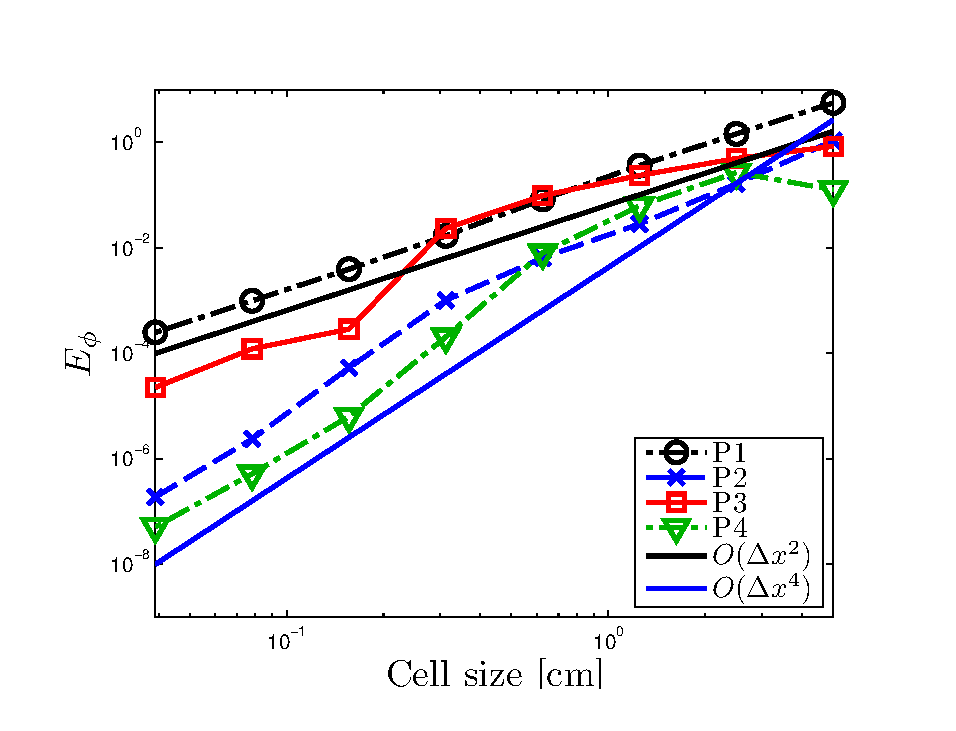
\includegraphics[width=10cm,trim=0.25in  0.5in 0.75in 0.75in,clip=true]{chapter6_grey_radtran/Dissertation_Data/MMS2_TL_phi_L2.pdf}
\caption{Convergence of $E_{\phi}$ for the TL scheme in problem MMS1.}
\label{fig:mms1_tl_phi}
\end{figure}
%
%
\begin{figure}[!hbp]
\centering
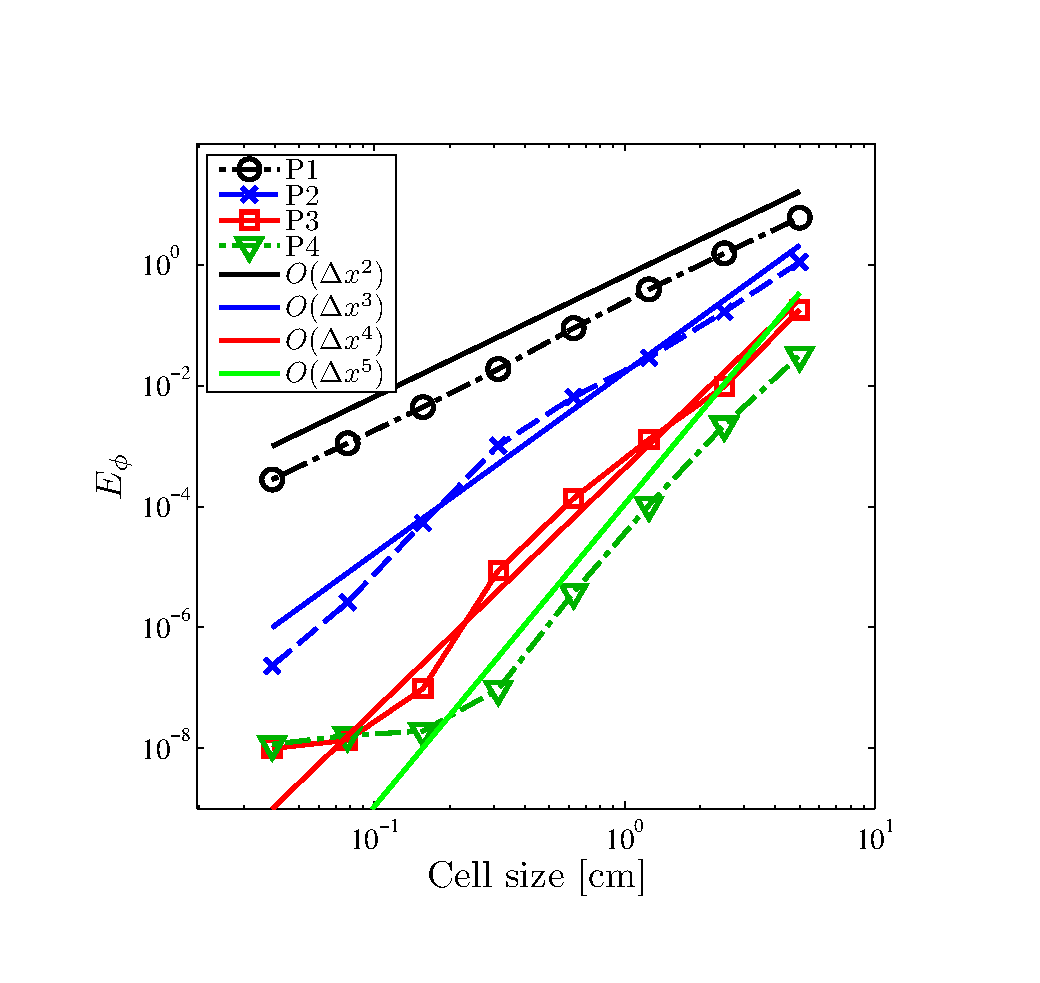
\includegraphics[width=10cm,trim=0.25in  0.5in 0.75in 0.75in,clip=true]{chapter6_grey_radtran/Dissertation_Data/MMS2_SLXS_Lobatto_phi_L2.pdf}
\caption{Convergence of $E_{\phi}$ for the SL Lobatto scheme in problem MMS1.}
\label{fig:mms1_lobatto_phi}
\end{figure}
%
%
\begin{figure}[!htp]
\centering
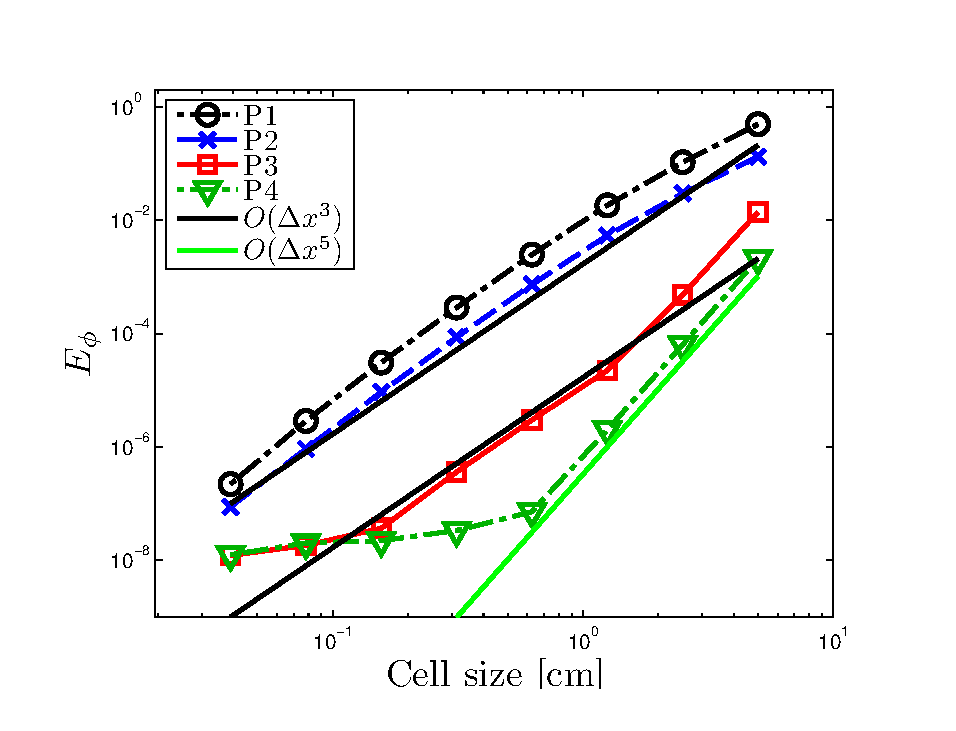
\includegraphics[width=10cm,trim=0.25in  0.5in 0.75in 0.75in,clip=true]{chapter6_grey_radtran/Dissertation_Data/MMS2_SLXS_Gauss_phi_L2.pdf}
\caption{Convergence of $E_{\phi}$ for the SL Gauss scheme in problem MMS1.}
\label{fig:mms1_gauss_phi}
\end{figure}
%
\begin{figure}[!hbp]
\centering
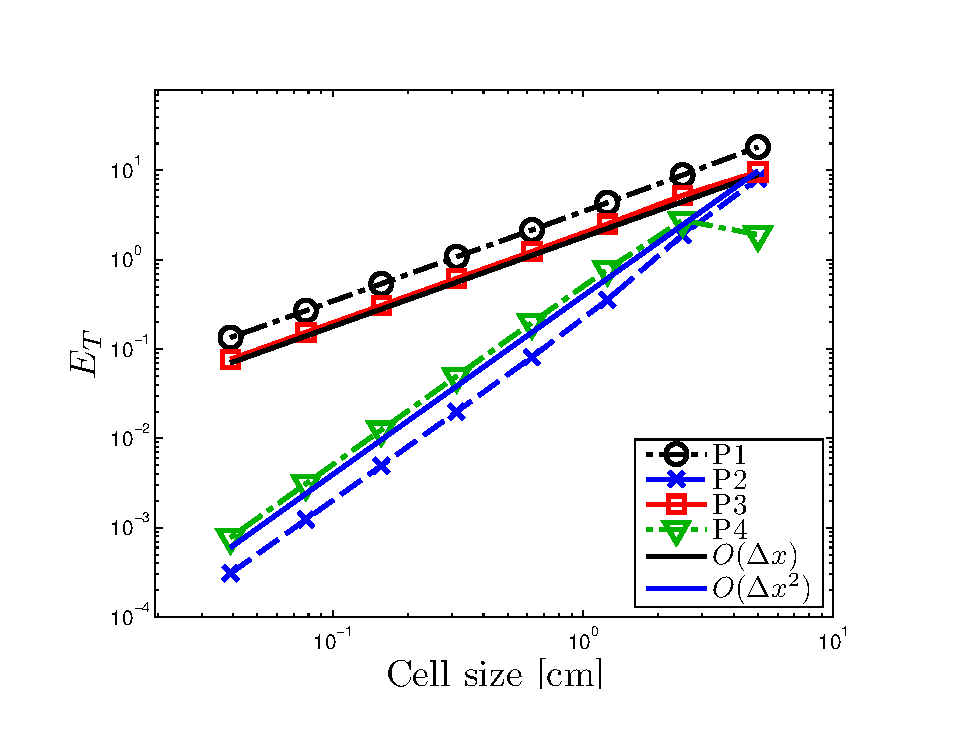
\includegraphics[width=10cm,trim=0.25in  0.5in 0.75in 0.75in,clip=true]{chapter6_grey_radtran/Dissertation_Data/MMS2_TL_temp_L2.pdf}
\caption{Convergence of $E_{T}$ for the TL scheme in problem MMS1.}
\label{fig:mms1_tl_temp}
\end{figure}
%
%
\begin{figure}[!htp]
\centering
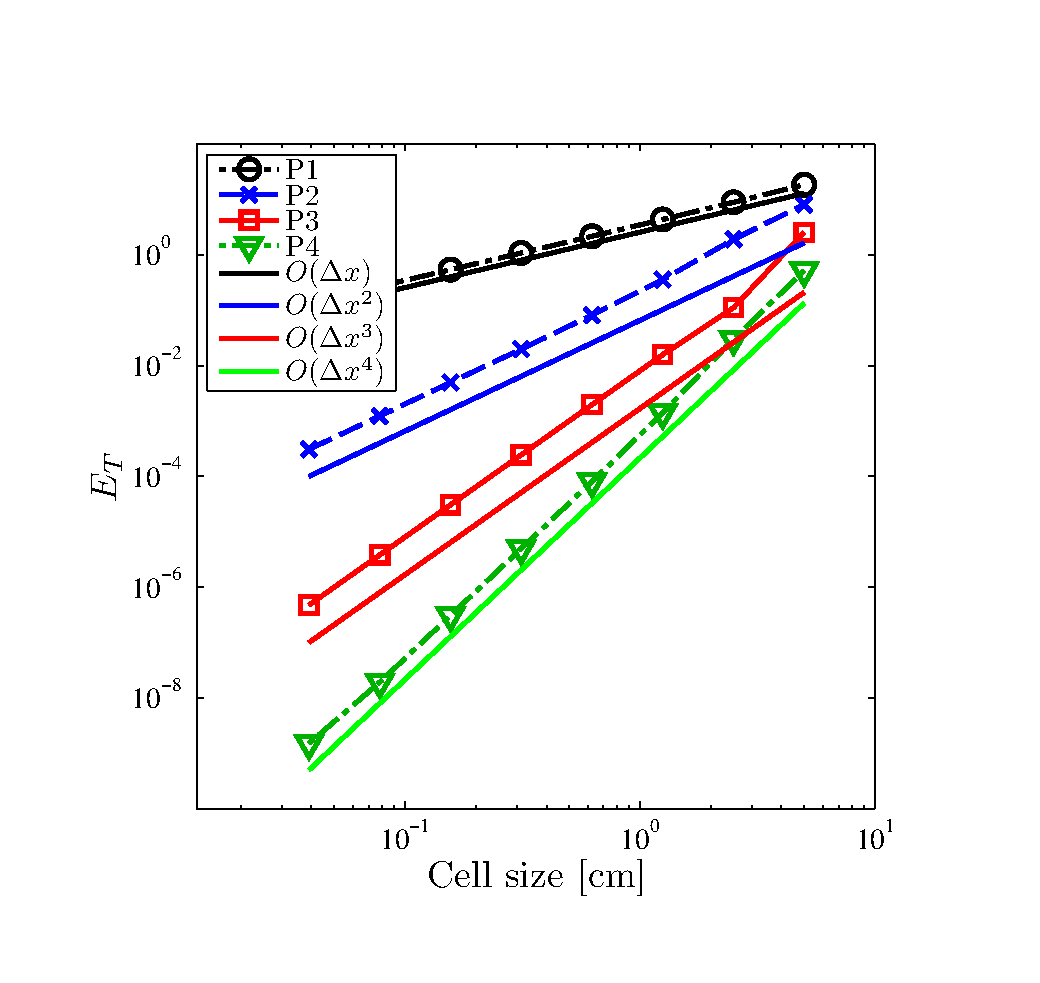
\includegraphics[width=10cm,trim=0.25in  0.5in 0.75in 0.75in,clip=true]{chapter6_grey_radtran/Dissertation_Data/MMS2_SLXS_Lobatto_temp_L2.pdf}
\caption{Convergence of $E_{T}$ for the SL Lobatto scheme in problem MMS1.}
\label{fig:mms1_lobatto_temp}
\end{figure}
%
%
\begin{figure}[!hbp]
\centering
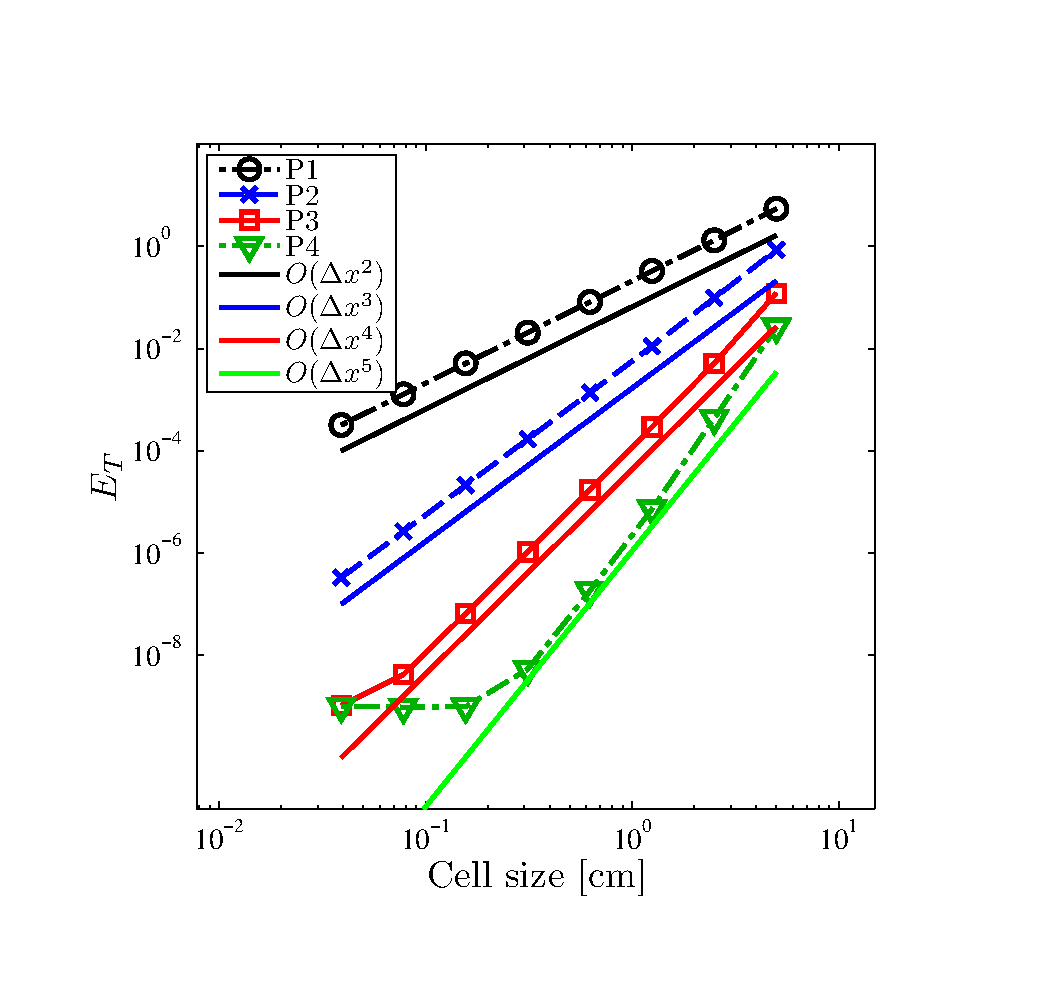
\includegraphics[width=10cm,trim=0.25in  0.5in 0.75in 0.75in,clip=true]{chapter6_grey_radtran/Dissertation_Data/MMS2_SLXS_Gauss_temp_L2.pdf}
\caption{Convergence of $E_{T}$ for the SL Gauss scheme in problem MMS1.}
\label{fig:mms1_gauss_temp}
\end{figure}

We make several observations regarding \figs{fig:mms1_tl_phi}{fig:mms1_gauss_temp}.  
First, the TL scheme does not necessarily increase in accuracy with an increase in trial space degree.
TL convergence of $E_{\phi}$ is limited to second order in space for odd degree trial space DFEM and third order spatial convergence for even degree trial space schemes, behavior identical to that demonstrated in our neutron transport testing.
A similar limit exists for TL convergence of $E_T$, at most first order for odd trial space degree and second order for even trial space degree.
Second, SL Lobatto converges the $L^2$ norm of the radiation energy density $\propto P+1$, the same order of convergence achieved in our neutron transport test problems for the convergence of $L^2$ error of the angular and scalar fluxes.
However, SL Lobatto only converges $E_T \propto P$, not $P+1$, as was the case for the neutron transport interaction rate.
Finally, SL Gauss converges $E_{\phi}$ and $E_T$ $\propto P+1$, the same order of convergence as seen with neutron transport.


In \figs{fig:mms1_tl_phi}{fig:mms1_gauss_temp}, and the other plots of this section, the plateauing of errors that appears in some plots is a combination of temporal error, for those problems that are time dependent, and our relative convergence tolerances for both temperature and angle integrated intensity. 
Given our convergence criteria, we would expect a plateau, $E_{T,min}$ of approximately
\benum
E_{T,min} \int_{x_{1/2} }^{x_{N_{cell}+1/2}}{ \epsilon_T \left[ F_t(t_{end}) W_T(x) \right] dx} \pep
\label{eq:err_plateau}
\eenum
Applying \eqt{eq:err_plateau} to MMS1, $E_{T,min} = 4.6\times 10^{-8}$, which is consistent with the location of the $E_T$ error plateau in \fig{fig:mms1_gauss_temp}.
Since the radiation solution is dependent on the accuracy of the temperature solution via the Planckian term and temperature dependent opacities, similar logic cannot be applied to estimating the location of the $E_{\phi}$ plateaus.
In \eqt{eq:err_plateau}, we are implicitly assuming that the error in $\phi$ is significantly less than the error in temperature. 

To understand the behaviors of SL Lobatto and SL Gauss completely, we now consider the $L^2$ like norm of cell average radiation energy density error, $E_{\phi_A}$ and cell average temperature error, $E_{T_A}$.
$E_{\phi_A}$ is approximated as:
\benum
E_{\phi_A} = \sqrt{
\sum_{c=1}^{N_{cell}}{ 
\frac{\Delta x}{2} 
\left( 
\frac{1}{2}\sum_{q=1}^{N_{qf}}{ w_q \widetilde{\phi}(s_q , t_{end})}  - \frac{1}{2}\sum_{q=1}^{N_{qf}}{ w_q \phi(s_q , t_{end})} 
\right)^2 
} 
} \pec
\eenum
with $N_{qf} = 2P + 7$, using Gauss quadrature.  $E_{T_A}$ is estimated in a similar fashion.
Convergence of $E_{\phi_A}$ is given in \fig{fig:mms1_lobatto_phi_A} for SL Lobatto and \fig{fig:mms1_gauss_phi_A} for SL Gauss.
Convergence of $E_{T_A}$ is given in \figs{fig:mms1_lobatto_temp_A}{fig:mms1_gauss_temp_A} for SL Lobatto and SL Gauss, respectively.
No definitive pattern emerges in the convergence of $E_{\phi_A}$ as a function of $P$ for SL Lobatto in \fig{fig:mms1_lobatto_phi_A} when considering linear through quartic polynomial trial spaces, though SL Lobatto convergence of $E_{\phi_A}$ looks to be $\propto 2P$ or slightly less.
SL Lobatto's apparent order of convergence for $E_{\phi_A}$ for TRT problems as shown in \fig{fig:mms1_lobatto_phi_A} is less than SL Lobatto convergence of $E_{\psi_A}$ for neutron transport (\figs{fig:multi_L2A_p1}{fig:multi_L2A_p4}), but not significantly. 
Similarly, the radiative transfer variant of SL Gauss does not converge $E_{\phi_A}$ for TRT simulations consistently $\propto 2P+1$ as SL Gauss converged $E_{\psi_A}$ neutron transport problems,
but it is close.  
Interestingly, the observed decreases in the convergence of $E_{\phi_A}$ for SL Lobatto and SL Gauss when applied to TRT relative to neutron transport convergence of $E_{\psi_A}$ does not hold when considering the convergence of $E_{T_A}$.  
SL Lobatto converges $E_{T_A}$ for TRT with the same order as SL Lobatto converges $E_{\psi_A}$ and $E_{IR_A}$ for neutron transport, $\propto 2P$.
SL Gauss actually exhibits an $E_{T_A}$ order of convergence that appears to exceed its neutron transport analog, converging $E_{T_A} \propto 2P+2$. \

\begin{figure}[!htp]
\centering
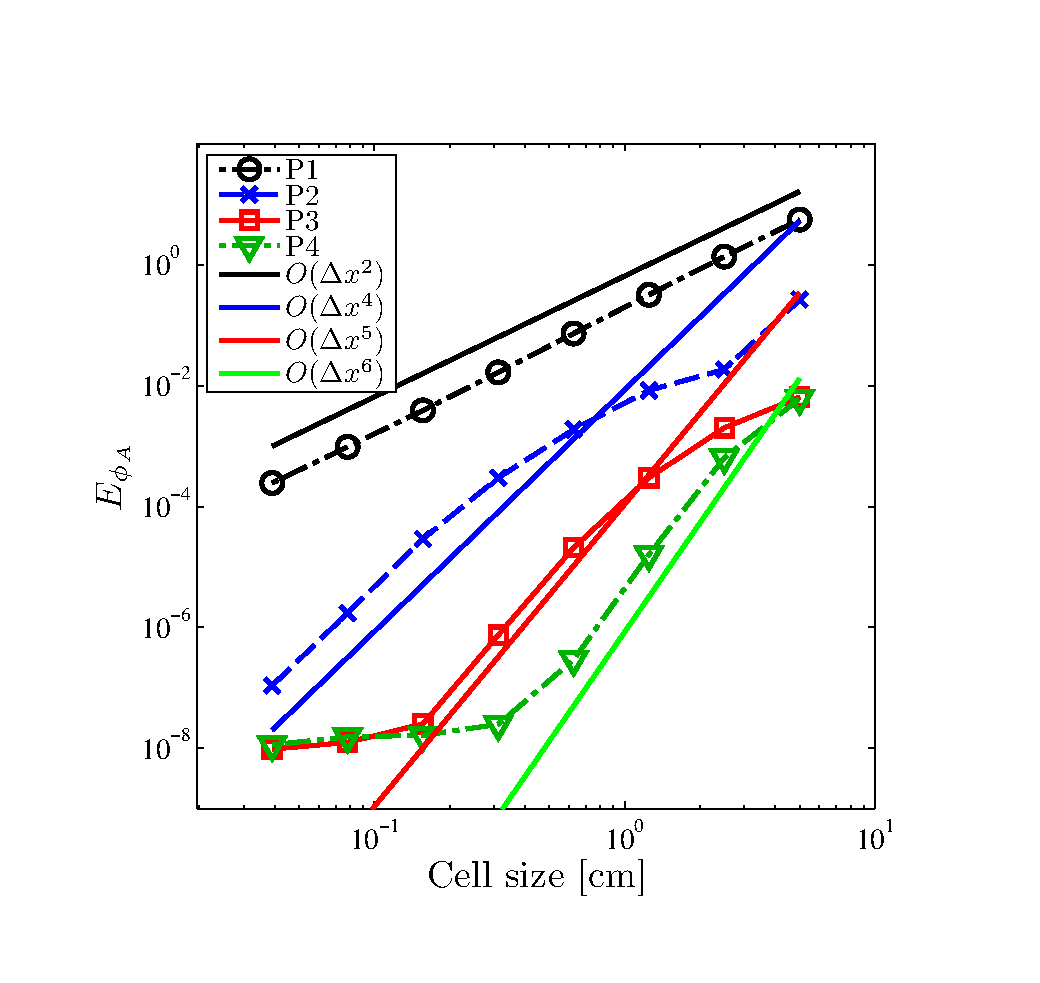
\includegraphics[width=9cm,trim=0.25in  0.5in 0.75in 0.75in,clip=true]{chapter6_grey_radtran/Dissertation_Data/MMS2_SLXS_Lobatto_phi_A.pdf}
\caption{Convergence of $E_{\phi_A}$ for the SL Lobatto scheme in problem MMS1.}
\label{fig:mms1_lobatto_phi_A}
\end{figure}
%
%
\begin{figure}[!hbp]
\centering
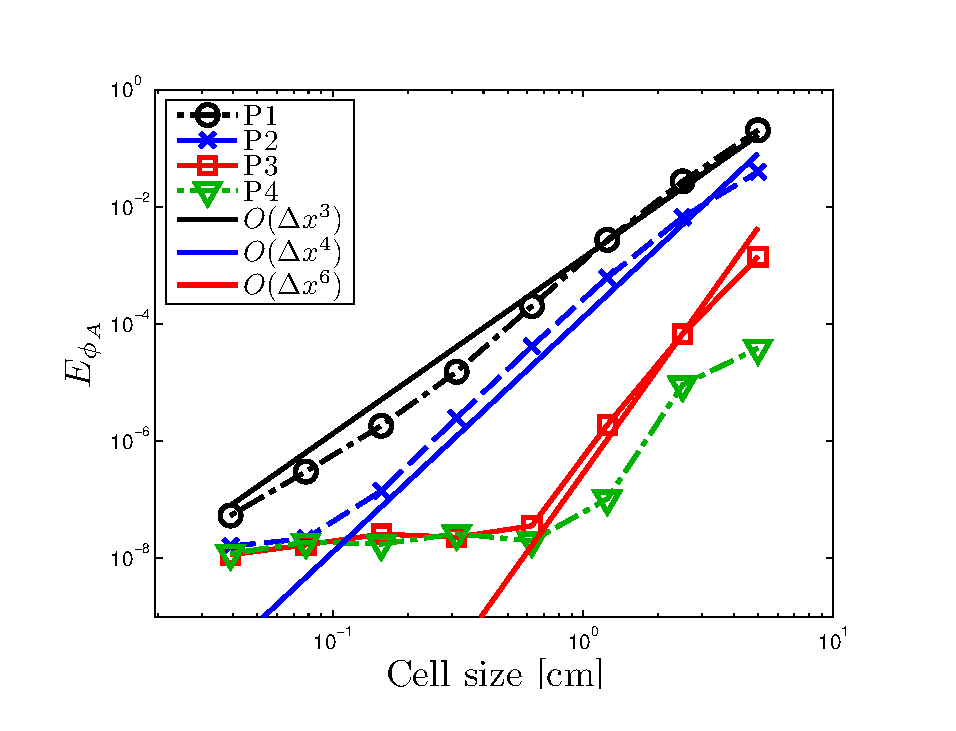
\includegraphics[width=9cm,trim=0.25in  0.1in 0.75in 0.5in,clip=true]{chapter6_grey_radtran/Dissertation_Data/MMS2_SLXS_Gauss_phi_A.pdf}
\caption{Convergence of $E_{\phi_A}$ for the SL Gauss scheme in problem MMS1.}
\label{fig:mms1_gauss_phi_A}
\end{figure}
%
%
\begin{figure}[!htp]
\centering
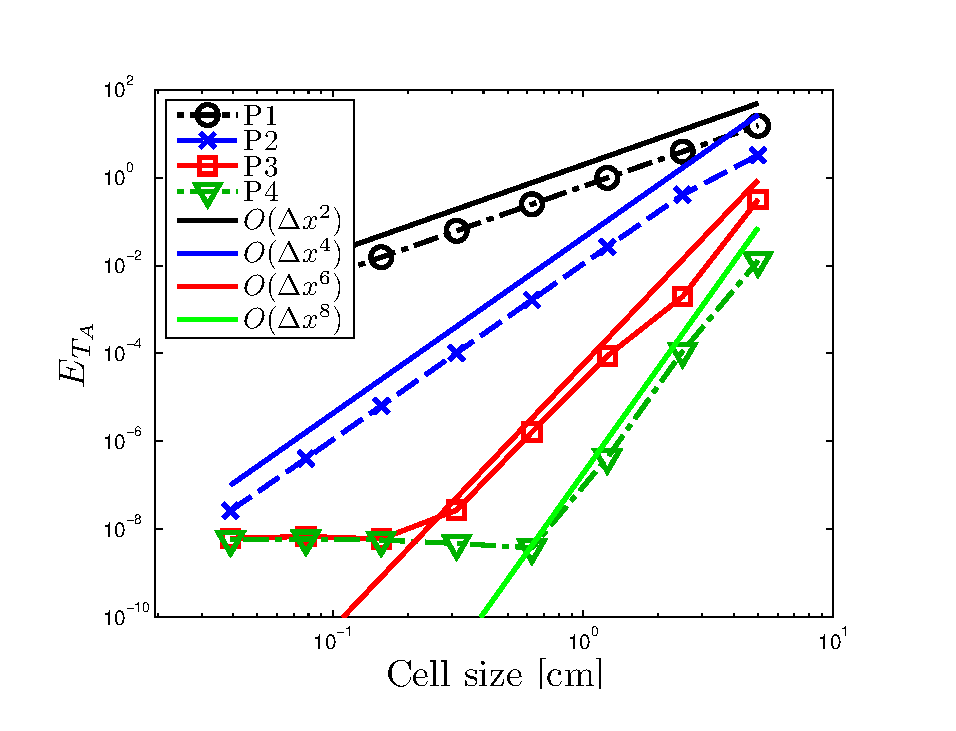
\includegraphics[width=10cm,trim=0.25in  0.5in 0.75in 0.75in,clip=true]{chapter6_grey_radtran/Dissertation_Data/MMS2_SLXS_Lobatto_temp_A.pdf}
\caption{Convergence of $E_{T_A}$ for the SL Lobatto scheme in problem MMS1.}
\label{fig:mms1_lobatto_temp_A}
\end{figure}
%
%
\begin{figure}[!hbp]
\centering
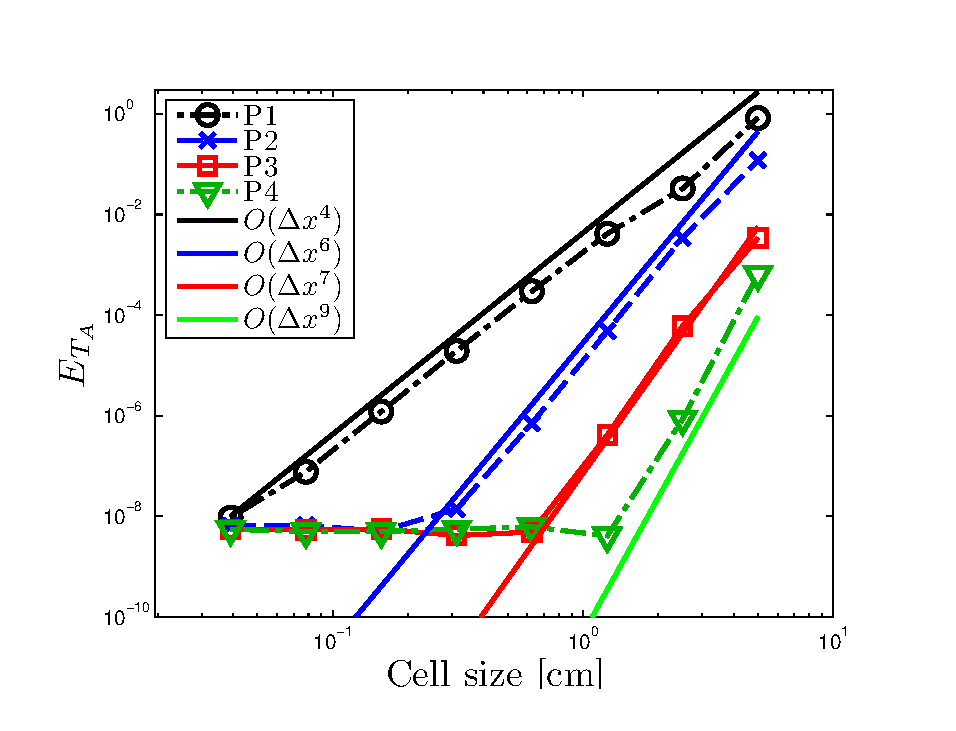
\includegraphics[width=10cm,trim=0.25in  0.5in 0.75in 0.75in,clip=true]{chapter6_grey_radtran/Dissertation_Data/MMS2_SLXS_Gauss_temp_A.pdf}
\caption{Convergence of $E_{T_A}$ for the SL Gauss scheme in problem MMS1.}
\label{fig:mms1_gauss_temp_A}
\end{figure}

It is our hypothesis that the apparent super convergence demonstrated by SL Gauss in converging $E_T$ is related to how we expand the Planckian in the same trial space as the DFEM temperature and radiation solutions. 
That is to say that we suspect the $N_P$ quadrature points of a given trial space degree SL Gauss scheme are significantly more accurate at integrating 
\benum
\B{i}(s) B(\widetilde{T}) \pec
\label{eq:planck_int}
\eenum
a degree $5P$ polynomial, than an $N_P$ Lobatto quadrature.
Though the $N_P$ point Gauss quadrature only exactly integrates polynomials of degree $2(P+1) -1$, it may be that the remaining terms are coincidentally very small in magnitude for a degree $5P$ polynomial of the particular nature of \eqt{eq:planck_int}.

%This plateauing of errors seen in the above plots is a result of two things.  
%First, the nested nature of our TRT solution algorithm.
%Due to the nested iterations, we must use the tightest tolerance on the innermost solve, the intensity update.
%We terminate the innermost solve after reaching a certain point-wise change tolerance, $\epsilon_{inner}$, of the zero-th angular moment of the angle integrated intensity: 
%\benum
%\max_{j} { \abs{ \frac{\phi_{j}^{(\ell+1)} - \phi_j^{(\ell)} }{\phi_{j}^{(\ell+1)} } }  } < \epsilon_{inner} \pep
%\eenum
%Similarly, the thermal iteration of SDIRK stage $s$ is terminated when every temperature solution at the DFEM interpolation points, $T_j$,  changes less than $\epsilon_{thermal}$,
%\benum
 %\max_{j} { { \abs{ \frac{ T_{j,s}^{(\ell+1)} - T_j^{(\ell)} }{T_{j}^{(\ell+1)} } }  } }< \epsilon_{thermal} \pep
%\eenum
%For this and all other MMS problems, $\epsilon_{inner} = 10^{-12}$ and $\epsilon_{thermal} = 10^{-10}$.
%Secondly, as the TRT equations are functions of space and time, it possible that the error of a given spatial discretization is smaller than the temporal error of the problem, thus a plateauing of the solution error as a function of spatial mesh refinement occurs.
%Thus, truly accurate solutions require the refinement of both spatial mesh and time step size.

\subsubsection{Trigonometric in  Space - Linear in Time - with Temperature Dependent Material Properties}

We now consider a problem with temperature dependent material properties, MMS2.  We impose the following solution:
\beanum
M(\mu_d) &=& \frac{1}{4\pi} \\
W_I(x) &=& 9 \cos\left( \frac{\pi x}{10} - \frac{\pi}{2} \right) + 3 \pec \\
W_T(x) &=&  5 \cos\left( \frac{\pi x}{10} - \frac{\pi}{2} \right) + 5 \pec \\
F(t) &=&  1 + .02t \pec
\eeanum
and define the following material properties:
\beanum
C_v &=& 0.2 + 0.01 T^3 \\
\sigma_a &=& \frac{10^4}{T^3} \\
\sigma_s &=& 0.5 \pep
\eeanum
In our problem, $x\in[0,10]$, $t\in[0,2]$, we use the three stage, third order accurate SDRIK method of Alexander \cite{alexander} with $\Delta t = 0.001$.  
In total , we consider four different DFEM schemes for this problem, SL Lobatto, SL Gauss, SLXS Lobatto, and SLXS Gauss.  
The methods denoted SL assume cell-wise constant opacities and heat capacities,  equal to the cell-wise volumetric average of that quantity.  
The SLXS schemes explicitly account for the within cell variation of temperature dependent material properties by evaluating $\mathbf{R}$ as in \eqt{eq:chap3_sl_react}.
$E_{\phi}$ for the SL Lobatto and SL Gauss schemes is plotted in \fig{fig:mms3_constant_lobatto_phi} and \fig{fig:mms3_constant_gauss_phi}, respectively.
\begin{figure}[!hbp]
\centering
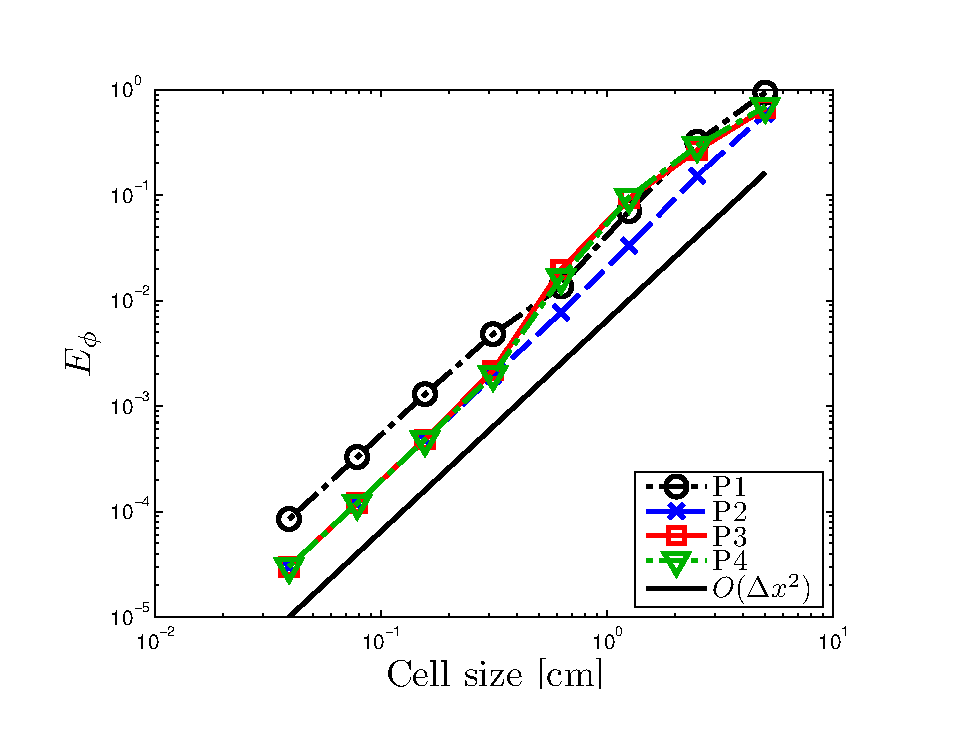
\includegraphics[width=10cm,trim=0.25in  0.25in 0.75in 0.5in,clip=true]{chapter6_grey_radtran/Dissertation_Data/MMS3_Constant_XS_SL_Lobatto_phi_L2.pdf}
\caption{Convergence of $E_{\phi}$ for the SL Lobatto scheme in problem MMS2.}
\label{fig:mms3_constant_lobatto_phi}
\end{figure}
%
%
\begin{figure}[!htp]
\centering
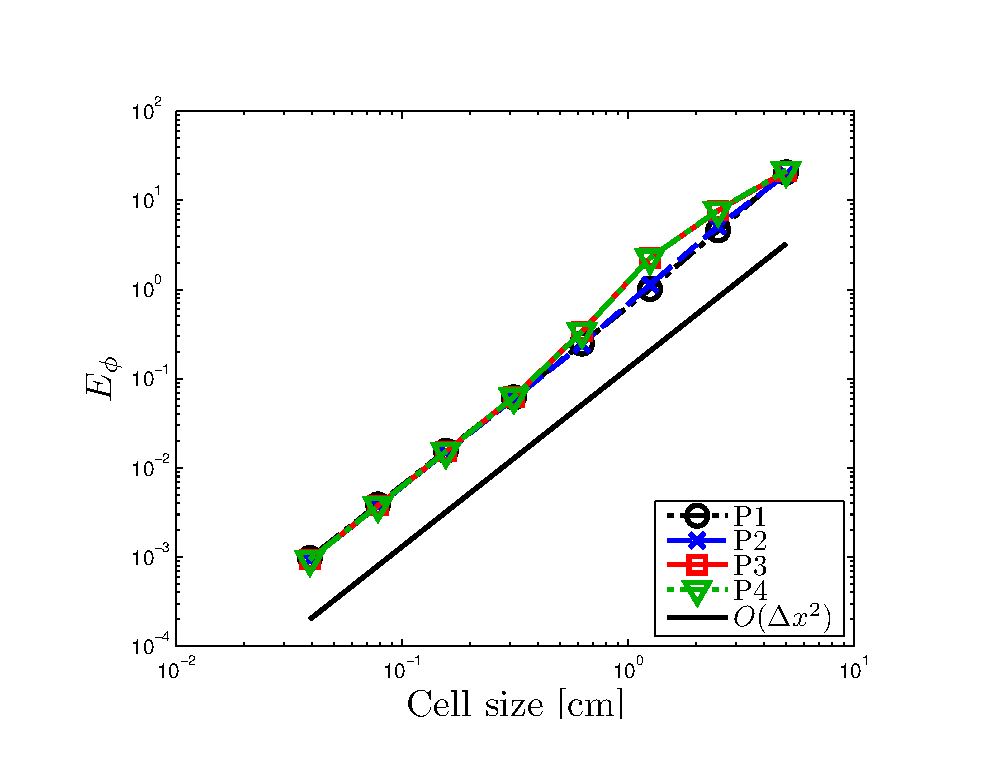
\includegraphics[width=10cm,trim=0.25in  0.25in 0.75in 0.5in,clip=true]{chapter6_grey_radtran/Dissertation_Data/MMS3_Constant_XS_SL_Gauss_phi_L2.pdf}
\caption{Convergence of $E_{\phi}$ for the SL Gauss scheme in problem MMS2.}
\label{fig:mms3_constant_gauss_phi}
\end{figure}
\begin{figure}[!hbp]
\centering
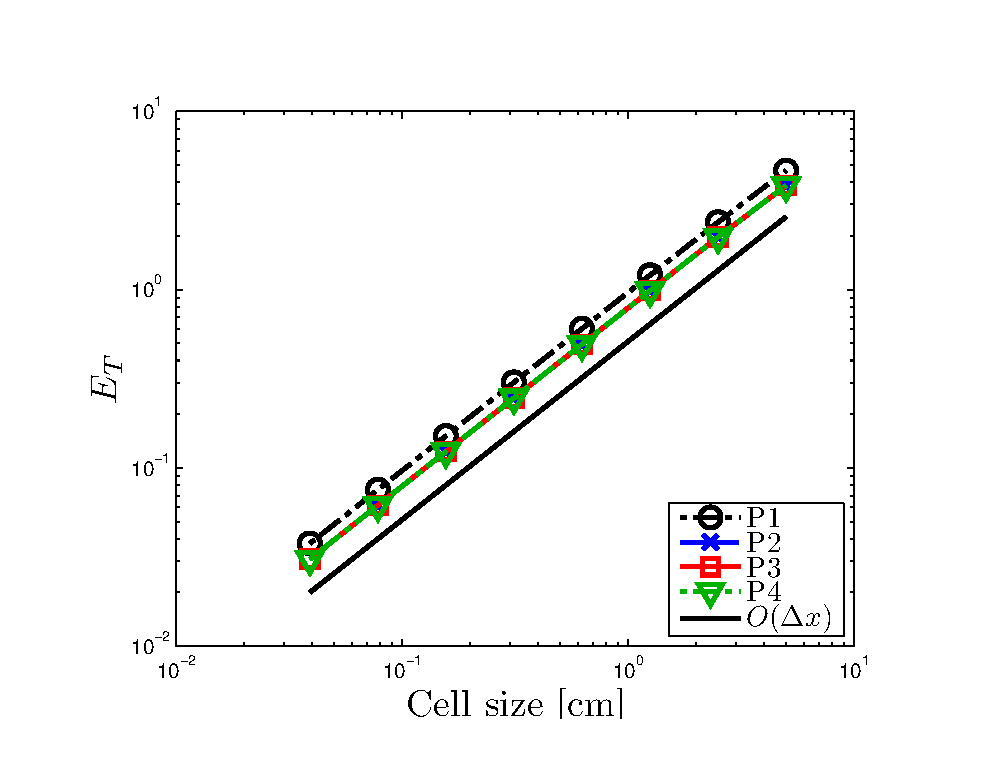
\includegraphics[width=10cm,trim=0.25in  0.2in 0.75in 0.5in,clip=true]{chapter6_grey_radtran/Dissertation_Data/MMS3_Constant_XS_SL_Lobatto_temp_L2.pdf}
\caption{Convergence of $E_{T}$ for the SL Lobatto scheme in problem MMS2.}
\label{fig:mms3_constant_lobatto_temp}
\end{figure}
%
%
\begin{figure}[!htp]
\centering
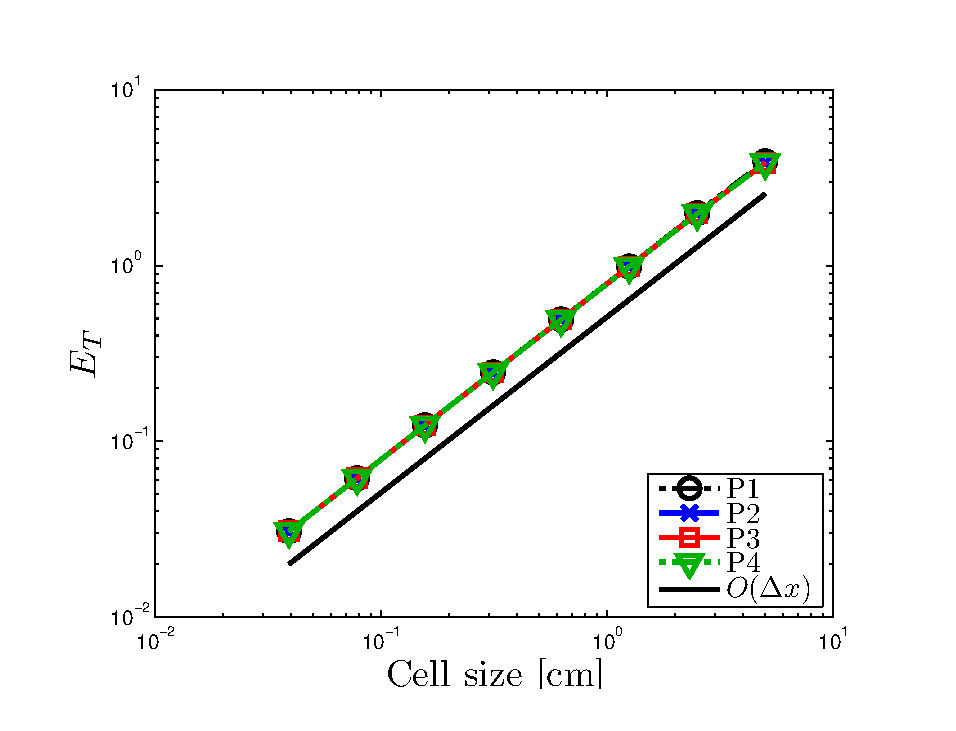
\includegraphics[width=10cm,trim=0.25in  0.2in 0.75in 0.5in,clip=true]{chapter6_grey_radtran/Dissertation_Data/MMS3_Constant_XS_SL_Gauss_temp_L2.pdf}
\caption{Convergence of $E_{T}$ for the SL Gauss scheme in problem MMS2.}
\label{fig:mms3_constant_gauss_temp}
\end{figure}

Regardless of DFEM interpolation point type or trial space degree, assuming cell-wise constant material properties limits spatial convergence of $E_{\phi}$ to at most second order.
Confirming our suspicion that assuming cell-wise constant material properties limit the convergence of $E_T$ as well, we plot the convergence of $E_T$ for the SL Lobatto scheme in \fig{fig:mms3_constant_lobatto_temp} and for the SL Gauss scheme in \fig{fig:mms3_constant_gauss_temp}.
Figures \ref{fig:mms3_constant_lobatto_temp}-\ref{fig:mms3_constant_gauss_temp} verify the hypothesis we developed while discussing our neutron transport results: assuming a cell-wise constant opacity limits $L^2$ convergence of temperature to at most first order in space, regardless of DFEM trial space degree.

To verify that the high order of convergence observed for $E_{IR_A}$ in Section 3 does not translate to a high rate of spatial convergence for $E_{T_A}$, we consider \fig{fig:mms3_constant_lobatto_temp_A} and \fig{fig:mms3_constant_gauss_temp_A}.
Figure \ref{fig:mms3_constant_lobatto_temp_A} verifies that regardless of trial space degree, the SL Lobatto scheme assuming a cell-wise constant opacity for a problem with temperature or spatially varying opacities converges $E_{T_A}$ second order in space.
Likewise, \fig{fig:mms3_constant_gauss_temp_A} demonstrates the same is true for the SL Gauss scheme.
\pagebreak
\begin{figure}[!htp]
\centering
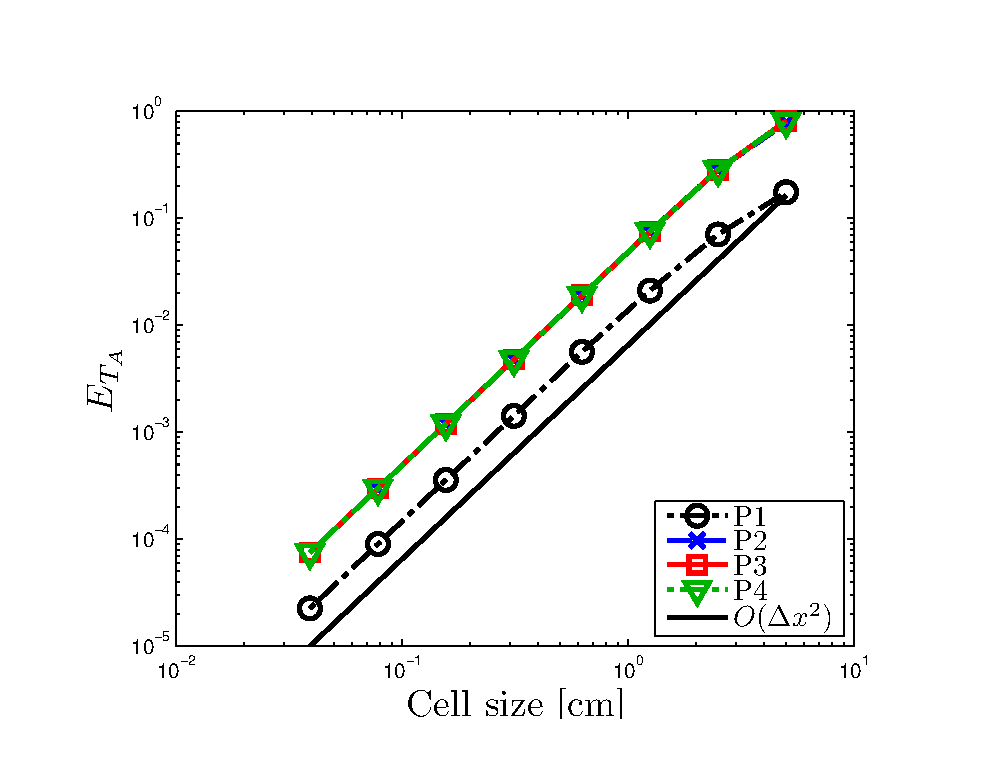
\includegraphics[width=9.5cm,trim=0.25in  0.2in 0.75in 0.5in,clip=true]{chapter6_grey_radtran/Dissertation_Data/MMS3_Constant_XS_SL_Lobatto_temp_A.pdf}
\caption{Convergence of $E_{T_A}$ for the SL Lobatto scheme in problem MMS2.}
\label{fig:mms3_constant_lobatto_temp_A}
\end{figure}
%
%
\begin{figure}[!hbp]
\centering
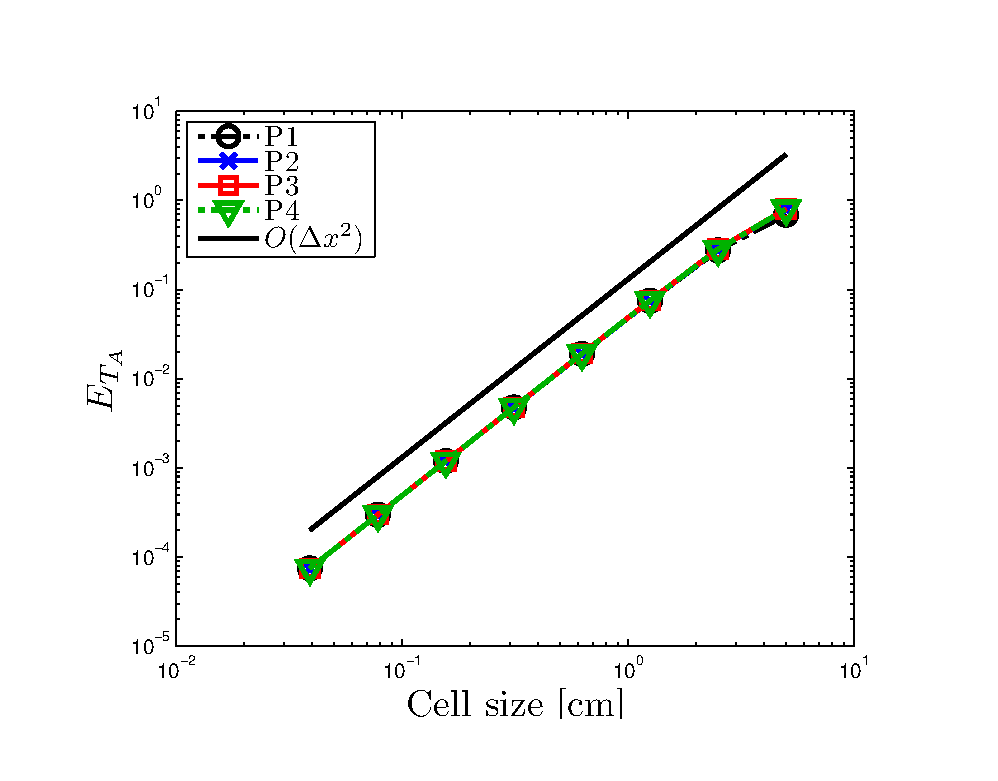
\includegraphics[width=9.5cm,trim=0.25in  0.2in 0.75in 0.5in,clip=true]{chapter6_grey_radtran/Dissertation_Data/MMS3_Constant_XS_SL_Gauss_temp_A.pdf}
\caption{Convergence of $E_{T_A}$ for the SL Gauss scheme in problem MMS2.}
\label{fig:mms3_constant_gauss_temp_A}
\end{figure}
\pagebreak

We now consider the convergence of SLXS Lobatto and SLXS Gauss.  First, we see that in \fig{fig:mms3_slxs_lobatto_e_phi}, SLXS Lobatto converges $E_{\phi} \propto P+1$, and in \fig{fig:mms3_slxs_gauss_e_phi}, SLXS Gauss converges $E_{\phi}$ $\propto P+1$ as well.
Moving on to the convergence of $E_T$, in \fig{fig:mms3_slxs_lobatto_e_t} SLXS Lobatto converges $E_T \propto P$, the same rate SL Lobatto converged $E_T$ for the TRT problem with constant material properties.  
In \fig{fig:mms3_slxs_gauss_e_t} SLXS Gauss converges $E_T$ very rapidly, and only the asymptotic convergence rate of linear and quadratic DFEM can be estimated, though both suggest SLXS Gauss converges $E_T \propto P+2$.
\begin{figure}[!hbp]
\centering
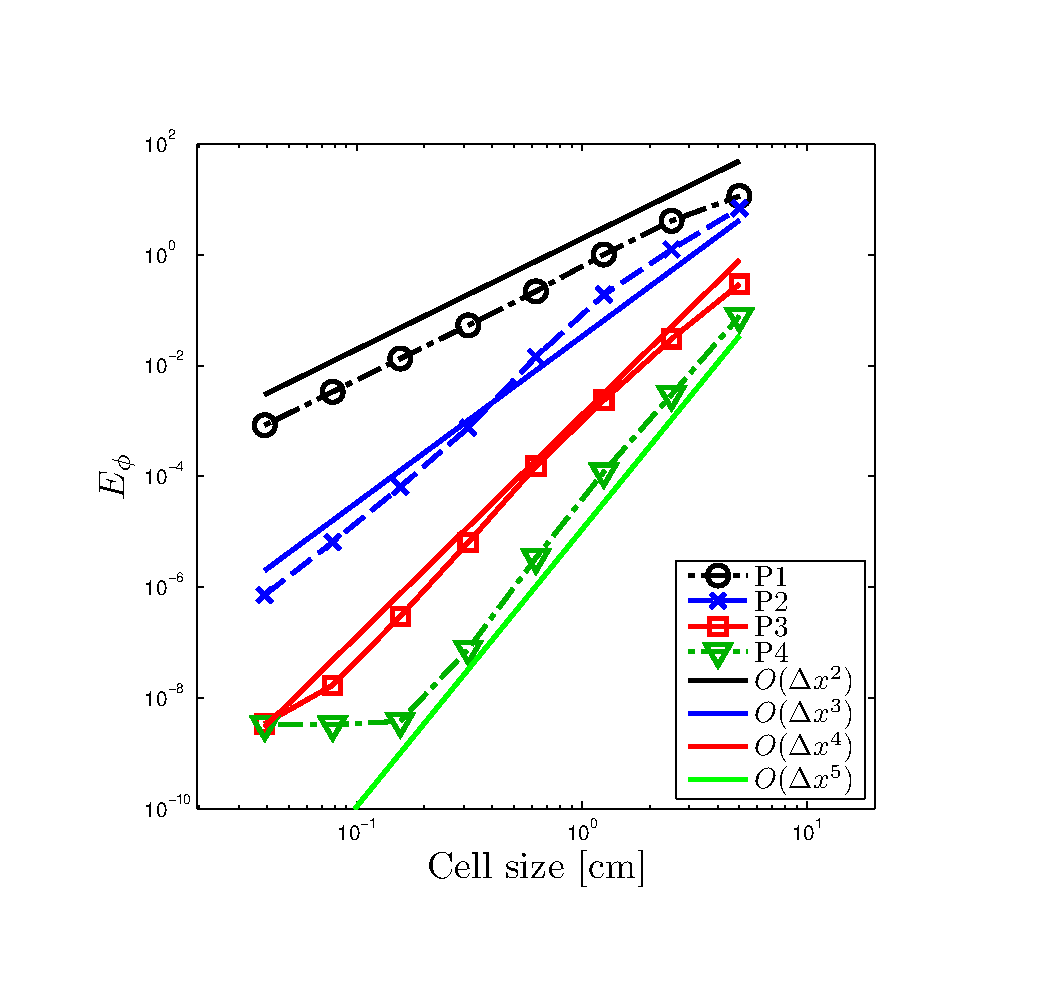
\includegraphics[width=10cm,trim=0.25in  0.25in 0.75in 0.75in,clip=true]{chapter6_grey_radtran/Dissertation_Data/MMS3_SLXS_Lobatto_phi_L2.pdf}
\caption{Convergence of $E_{\phi}$ for the SLXS Lobatto scheme in problem MMS2.}
\label{fig:mms3_slxs_lobatto_e_phi}
\end{figure}
%
%
\begin{figure}[!htp]
\centering
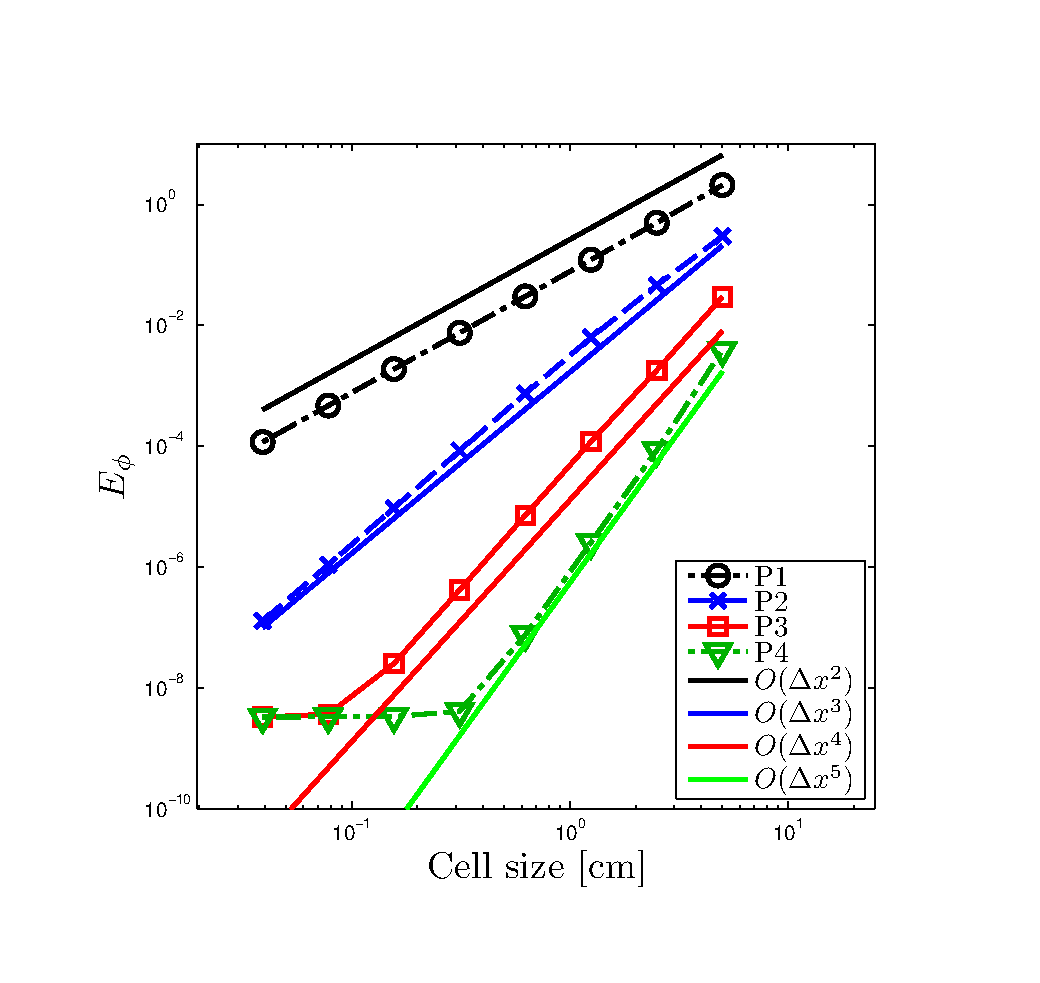
\includegraphics[width=10cm,trim=0.25in  0.25in 0.75in 0.75in,clip=true]{chapter6_grey_radtran/Dissertation_Data/MMS3_SLXS_Gauss_phi_L2.pdf}
\caption{Convergence of $E_{\phi}$ for the SLXS Gauss scheme in problem MMS2.}
\label{fig:mms3_slxs_gauss_e_phi}
\end{figure}
\begin{figure}[!hbp]
\centering
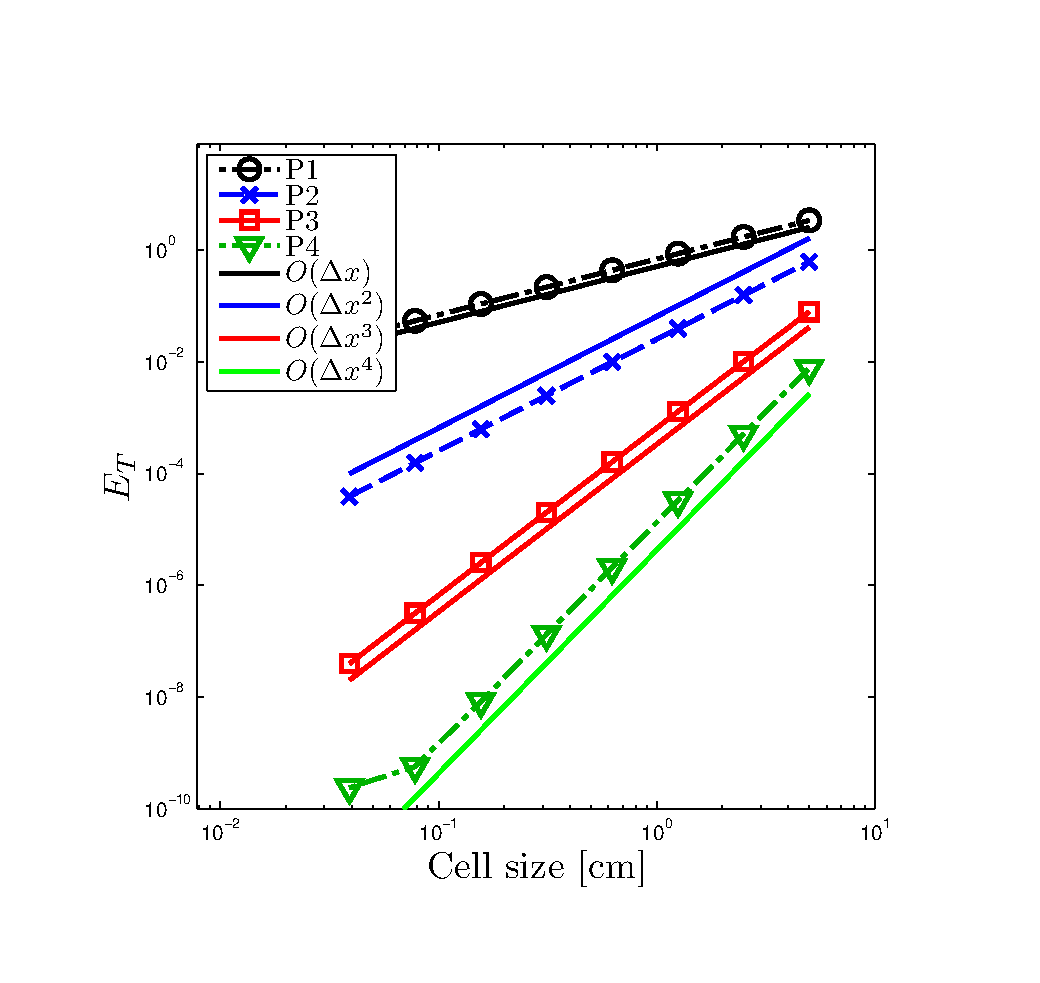
\includegraphics[width=10cm,trim=0.25in  0.25in 0.75in 0.75in,clip=true]{chapter6_grey_radtran/Dissertation_Data/MMS3_SLXS_Lobatto_temp_L2.pdf}
\caption{Convergence of $E_{T}$ for the SLXS Lobatto scheme in problem MMS2.}
\label{fig:mms3_slxs_lobatto_e_t}
\end{figure}
%
%
\begin{figure}[!htp]
\centering
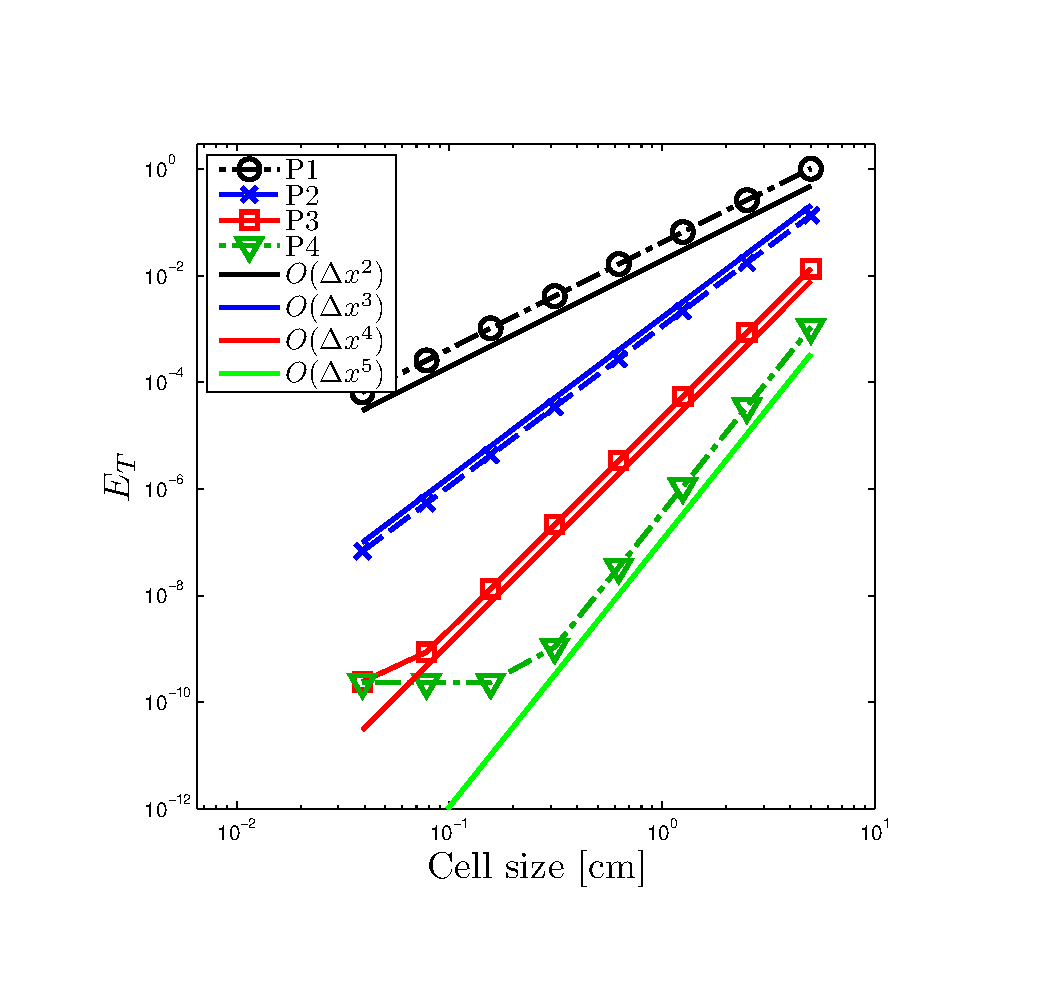
\includegraphics[width=9.5cm,trim=0.25in  0.25in 0.75in 0.75in,clip=true]{chapter6_grey_radtran/Dissertation_Data/MMS3_SLXS_Gauss_temp_L2.pdf}
\caption{Convergence of $E_{T}$ for the SLXS Gauss scheme in problem MMS2.}
\label{fig:mms3_slxs_gauss_e_t}
\end{figure}
%
%
%
\begin{figure}[!hbp]
\centering
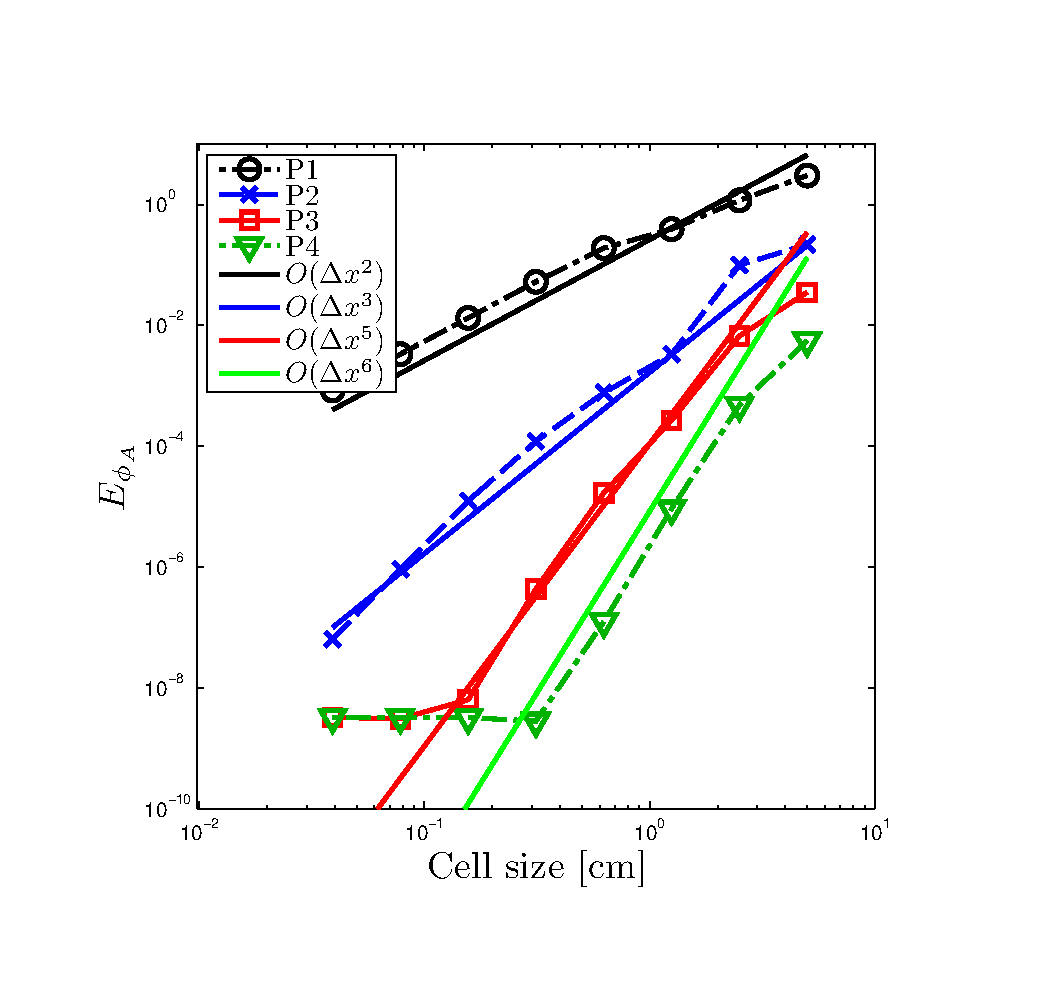
\includegraphics[width=9.5cm,trim=0.25in  0.4in 0.75in 0.75in,clip=true]{chapter6_grey_radtran/Dissertation_Data/MMS3_SLXS_SLXS_Lobatto_phi_A.pdf}
\caption{Convergence of $E_{\phi_A}$ for the SLXS Lobatto scheme in problem MMS2.}
\label{fig:mms3_slxs_lobatto_phi_a}
\end{figure}
%
%
\begin{figure}[!htp]
\centering
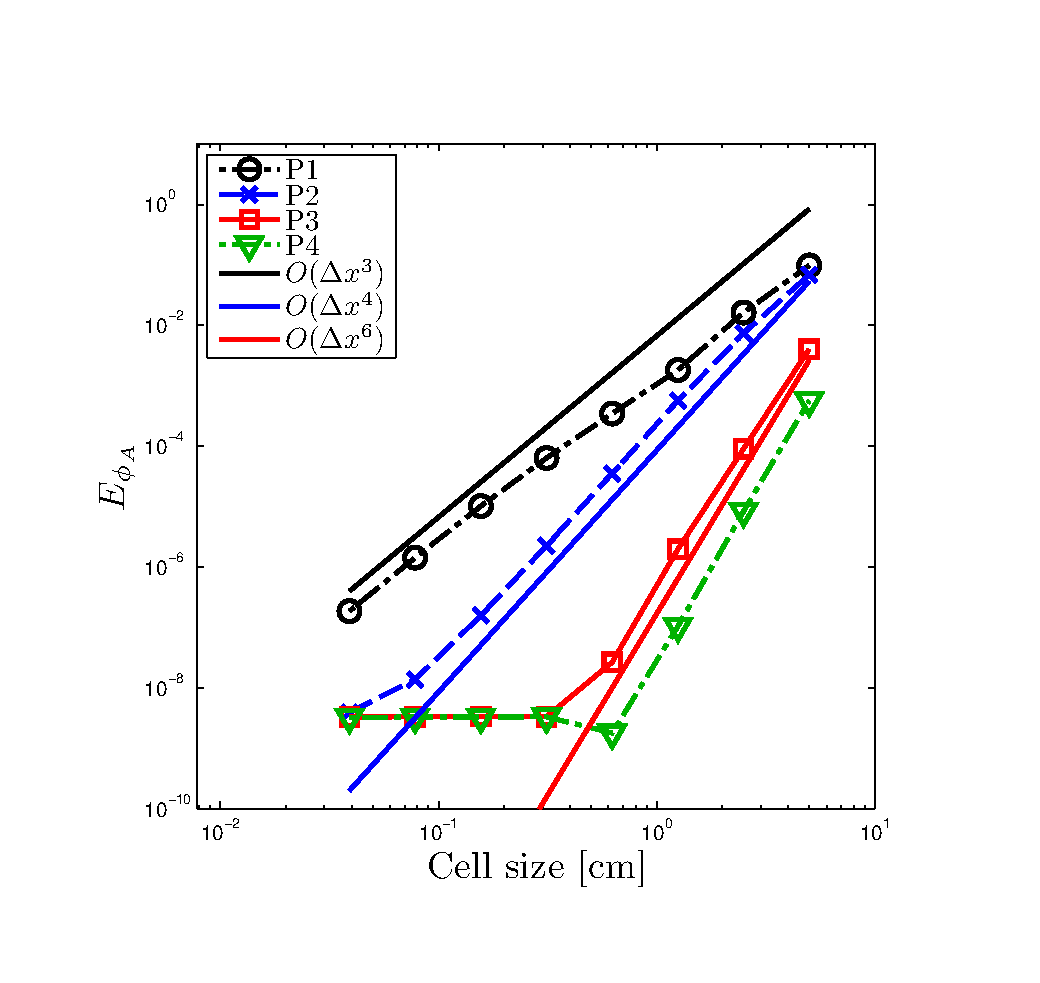
\includegraphics[width=10cm,trim=0.25in  0.25in 0.75in 0.75in,clip=true]{chapter6_grey_radtran/Dissertation_Data/MMS3_SLXS_Gauss_phi_A.pdf}
\caption{Convergence of $E_{\phi_A}$ for the SLXS Gauss scheme in problem MMS2.}
\label{fig:mms3_slxs_gauss_phi_a}
\end{figure}
\begin{figure}[!hbp]
\centering
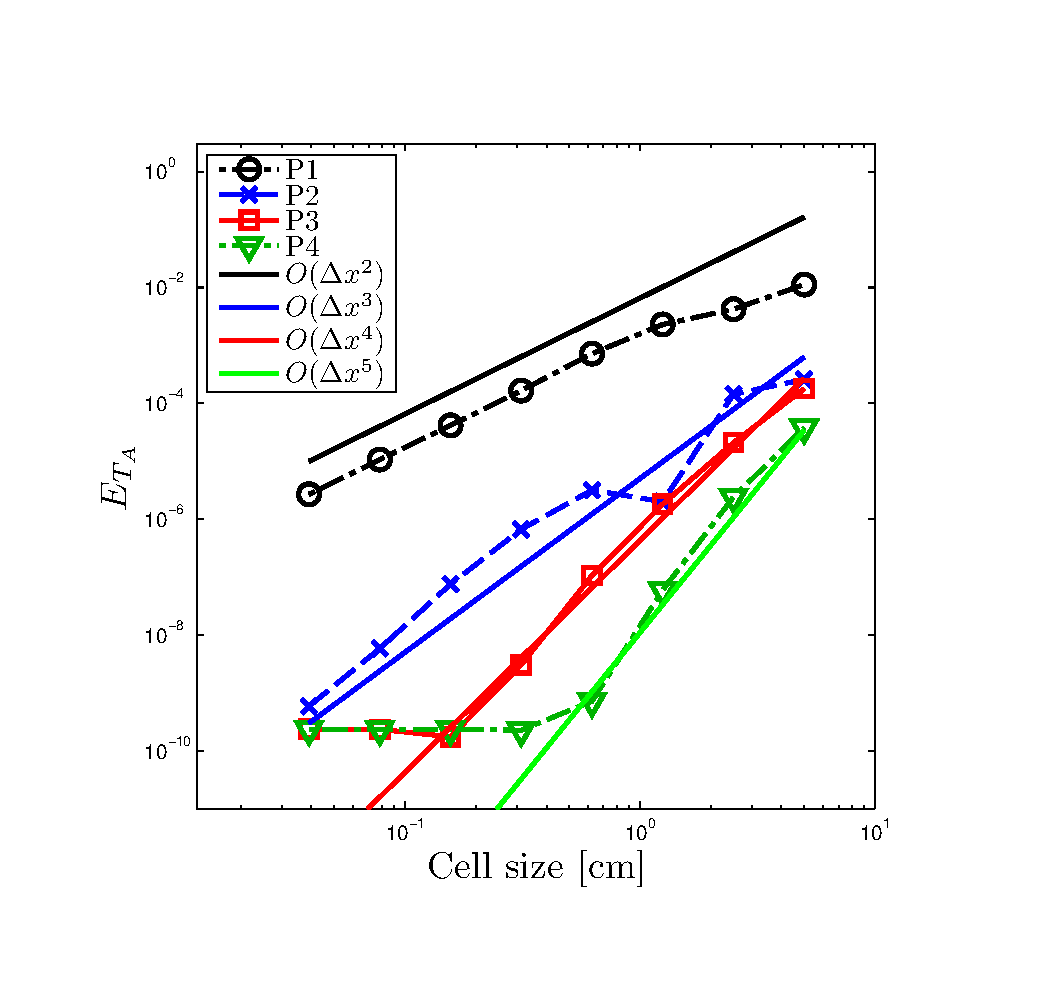
\includegraphics[width=10cm,trim=0.25in  0.25in 0.75in 0.75in,clip=true]{chapter6_grey_radtran/Dissertation_Data/MMS3_SLXS_Lobatto_temp_A.pdf}
\caption{Convergence of $E_{T_A}$ for the SLXS Lobatto scheme in problem MMS2.}
\label{fig:mms3_slxs_lobatto_t_a}
\end{figure}
%
%
\begin{figure}[!htp]
\centering
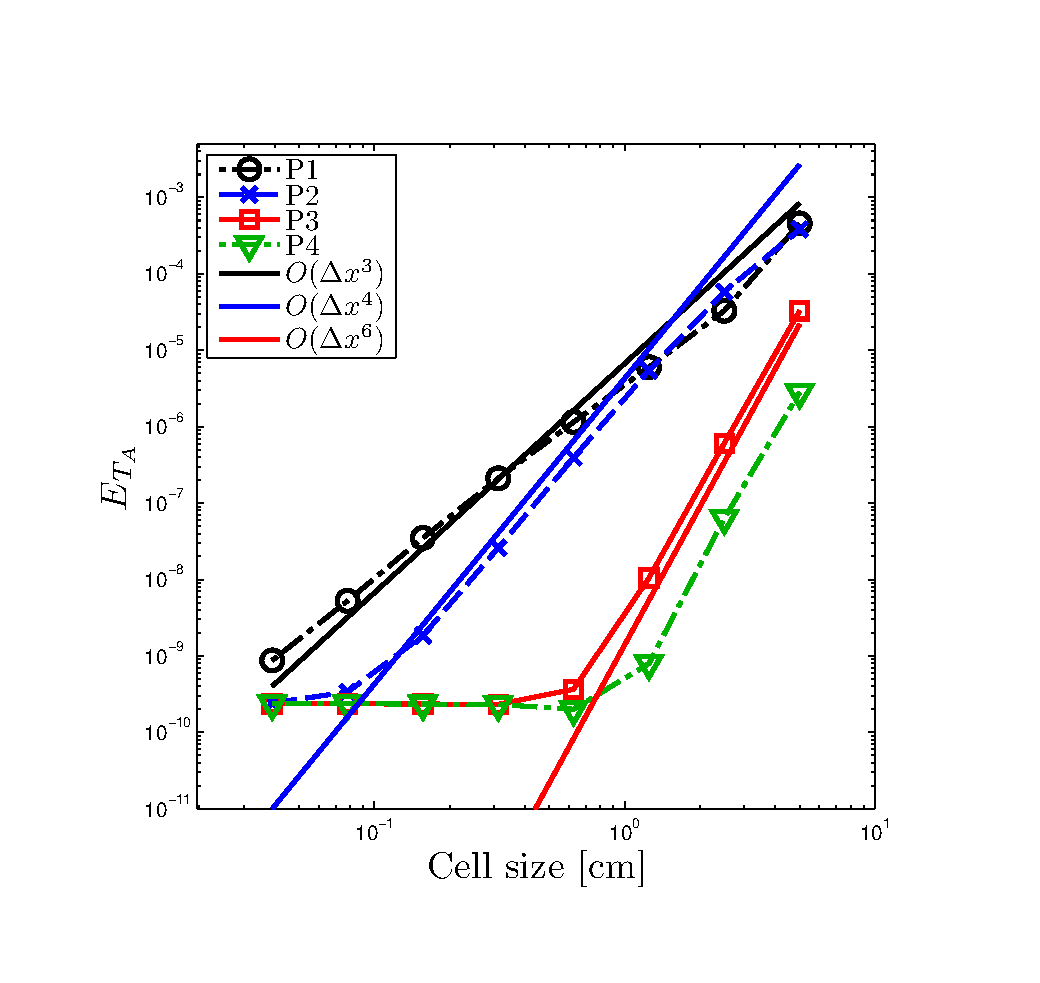
\includegraphics[width=10cm,trim=0.25in  0.25in 0.75in 0.75in,clip=true]{chapter6_grey_radtran/Dissertation_Data/MMS3_SLXS_Gauss_temp_A.pdf}
\caption{Convergence of $E_{T_A}$ for the SLXS Gauss scheme in problem MMS2.}
\label{fig:mms3_slxs_gauss_t_a}
\end{figure}

Focusing now on the convergence of cell average error quantities, we first consider $E_{\phi_A}$ for SLXS Lobatto and SLXS Gauss in \fig{fig:mms3_slxs_lobatto_phi_a} and \fig{fig:mms3_slxs_gauss_phi_a}, respectively.
Both SLXS Lobatto and SLXS Gauss converge $E_{\phi_A}$ at an order less than or at most equal to the order their respective neutron transport analogs converged $E_{\psi_A}$.
However, since both methods require only a small amount of mesh refinement to reach an error level approximately equal to our temperature tolerance, it is difficult to establish with certainty the order of convergence of either method for higher $P$.
For completeness, we include convergence plots of $E_{T_A}$ for SLXS Lobatto and SLXS Gauss respectively in \fig{fig:mms3_slxs_lobatto_t_a} and \fig{fig:mms3_slxs_gauss_t_a}.
All we definitively conclude from \figs{fig:mms3_slxs_lobatto_t_a}{fig:mms3_slxs_gauss_t_a} is that both SLXS Lobatto and SLXS Gauss experience increases in convergence of $E_{T_A}$ with increases in trial space degree.

\subsubsection{Constant in Time - Trigonometric in Space - with Temperature Dependent Material Properties}

We now consider a problem that is constant in time and varies as a cosine in space with temperature dependent material properties.  
Though very similar to MMS2, we hope that by considering a truly steady state problem, we can study the spatial error of our DFEM schemes without temporal error interference.
We impose a solution of the form:
\beanum
M(\mu_d) &=& \frac{1}{4\pi} \\
W_I(x) &=& 19 \cos\left( \frac{\pi x}{2} \right) + 20 \pec \\
W_T(x) &=&  15 \cos\left( \frac{\pi x}{2}  \right) + 20 \pec \\
F(t) &=&  10
\eeanum
and define the following material properties:
\beanum
C_v &=& 0.1 + 0.2 T^2 \\
\sigma_a &=& \frac{5}{T^2} \\
\sigma_s &=& 0.01 \pep
\eeanum
Repeating as we have before, we first consider the convergence of $E_{\phi}$ for SLXS Lobatto and SLXS Gauss in \fig{fig:constant_time_lobatto_phi} and \fig{fig:constant_time_gauss_phi}.
\begin{figure}[!htp]
\centering
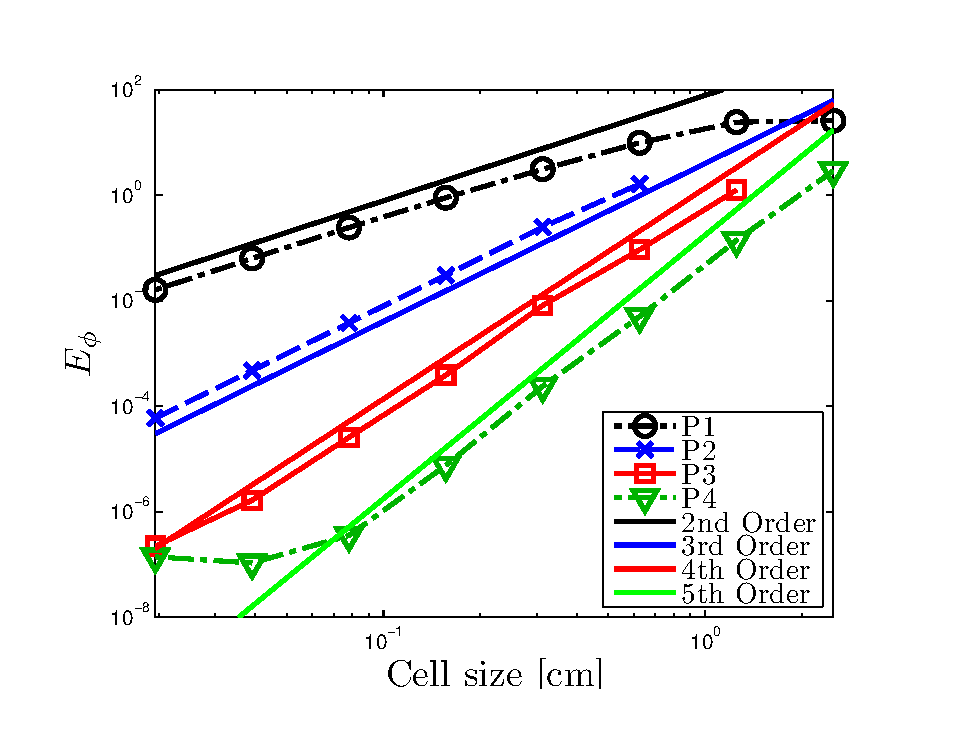
\includegraphics[width=10cm,trim=0.25in  0.2in 0.75in 0.5in,clip=true]{chapter6_grey_radtran/Dissertation_Data/Constant_Time_SLXS_Lobatto_phi_L2.pdf}
\caption{Convergence of $E_{\phi}$ for SLXS Lobatto scheme for steady state test problem.}
\label{fig:constant_time_lobatto_phi}
\end{figure}
%
%
\begin{figure}[!hbp]
\centering
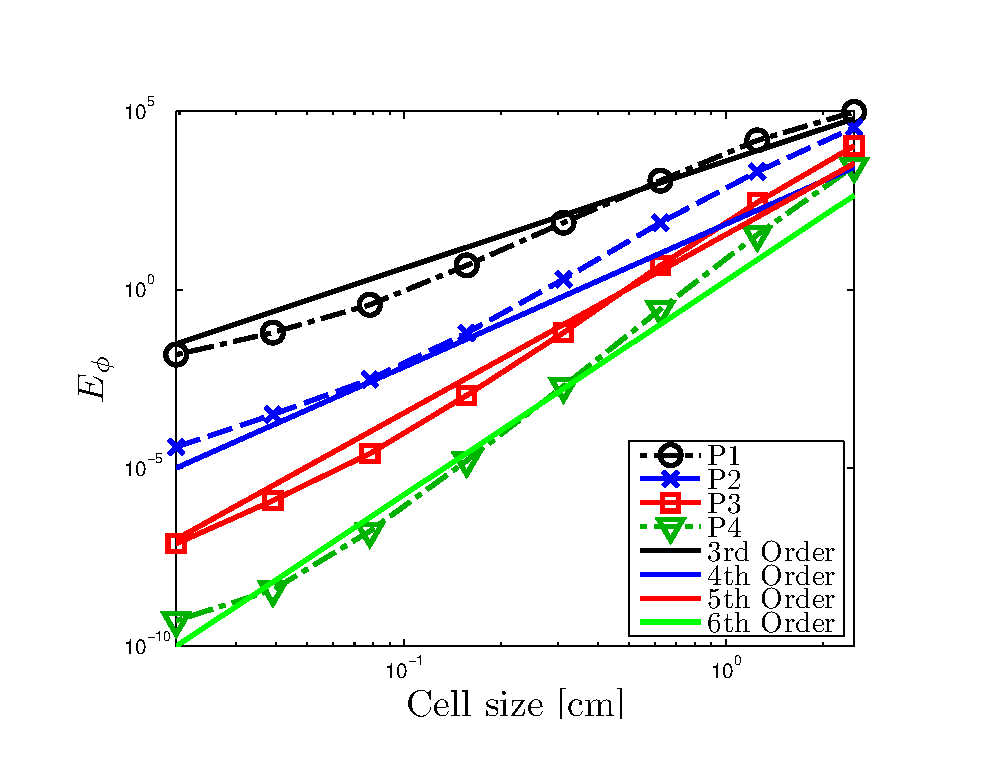
\includegraphics[width=10cm,trim=0.25in  0.2in 0.75in 0.5in,clip=true]{chapter6_grey_radtran/Dissertation_Data/Constant_Time_SLXS_Gauss_phi_L2.pdf}
\caption{Convergence of $E_{\phi}$ for SLXS Gauss scheme, for steady state test problem.}
\label{fig:constant_time_gauss_phi}
\end{figure}
As before, SLXS Lobatto converges $E_{\phi} \propto P+1$.  
However, SLXS Gauss appears to converges $E_{\phi} \propto P+2$.
It is not clear why SLXS Gauss convergence of $E_{\phi}$ increases when moving from the time dependent MMS1 and MMS2 problems to the steady-state test problem.

Now considering the convergence of $E_{T}$, the steady-state problem confirms SLXS Lobatto converges $E_T$ $\propto P$, shown in \fig{fig:constant_time_lobatto_t}, and SLXS Gauss converges $E_T \propto P+2$, as shown in \fig{fig:constant_time_gauss_t}.
\begin{figure}[!htp]
\centering
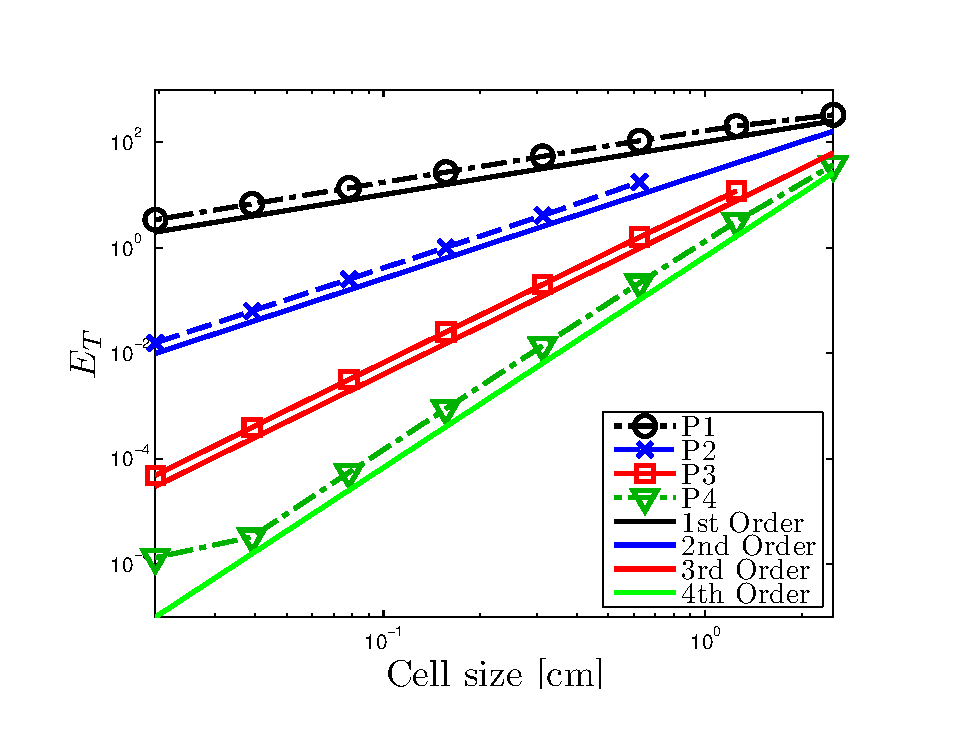
\includegraphics[width=10cm,trim=0.25in  0.2in 0.75in 0.5in,clip=true]{chapter6_grey_radtran/Dissertation_Data/Constant_Time_SLXS_Lobatto_temp_L2.pdf}
\caption{Convergence of $E_{T}$ for SLXS Lobatto scheme, for steady state test problem.}
\label{fig:constant_time_lobatto_t}
\end{figure}
%
\begin{figure}[!hbp]
\centering
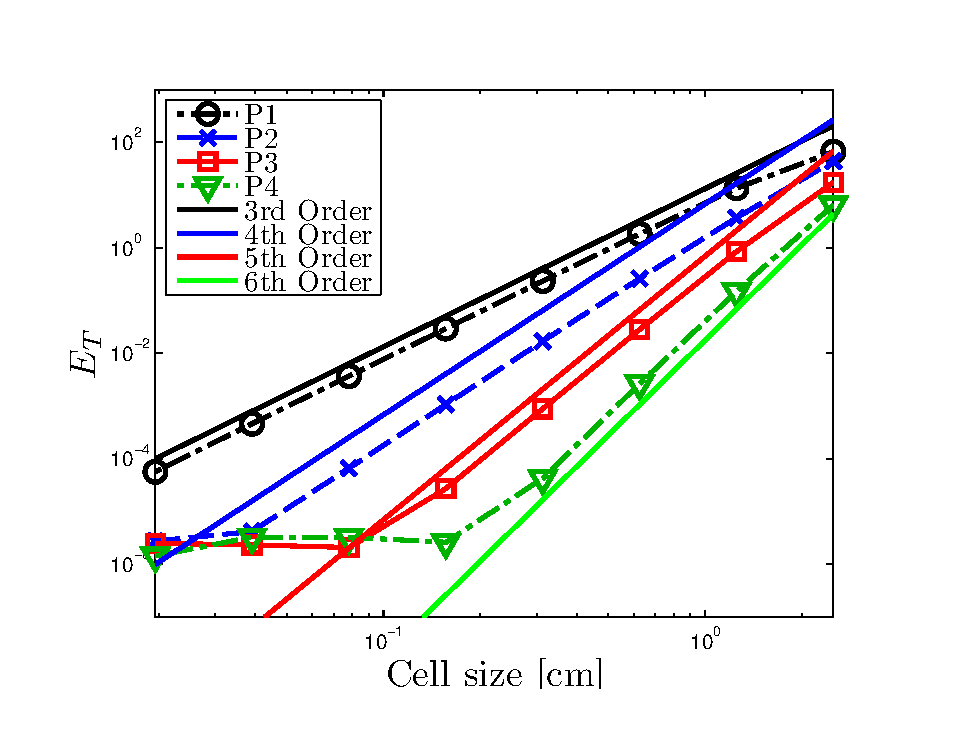
\includegraphics[width=9.5cm,trim=0.25in  0.2in 0.75in 0.5in,clip=true]{chapter6_grey_radtran/Dissertation_Data/Constant_Time_SLXS_Gauss_temp_L2.pdf}
\caption{Convergence of $E_{T}$ for SLXS Gauss scheme, for steady state test problem.}
\label{fig:constant_time_gauss_t}
\end{figure}

We now examine the convergence of $E_{\phi_A}$.  
The estimated order of convergence of $E_{\phi_A}$ in \fig{fig:constant_time_lobatto_phi_a} for SLXS Lobatto, appears to be $\propto 2P$, greater than the results from MMS1 and MMS2, but equal to what we would have hypothesized from neutron transport.  
%Figure \ref{fig:constant_time_lobatto_phi_a} and \fig{fig:mms3_slxs_lobatto_phi_a} giving different estimates of $E_{\phi_A}$ convergence is most likely due to a lack of data points available prior to reaching our iterative tolerances, preventing a clear inference of asymptotic convergence rate.
Similarly the convergence of $E_{\phi_A}$ for SLXS Gauss estimated in \fig{fig:constant_time_gauss_phi_a} appears to be greater, $\propto 2P+2$, than the SLXS Gauss order of convergence for $E_{\phi_A}$, $<2P+1$, given in \fig{fig:mms3_slxs_gauss_phi_a}.
\begin{figure}[!hbp]
\centering
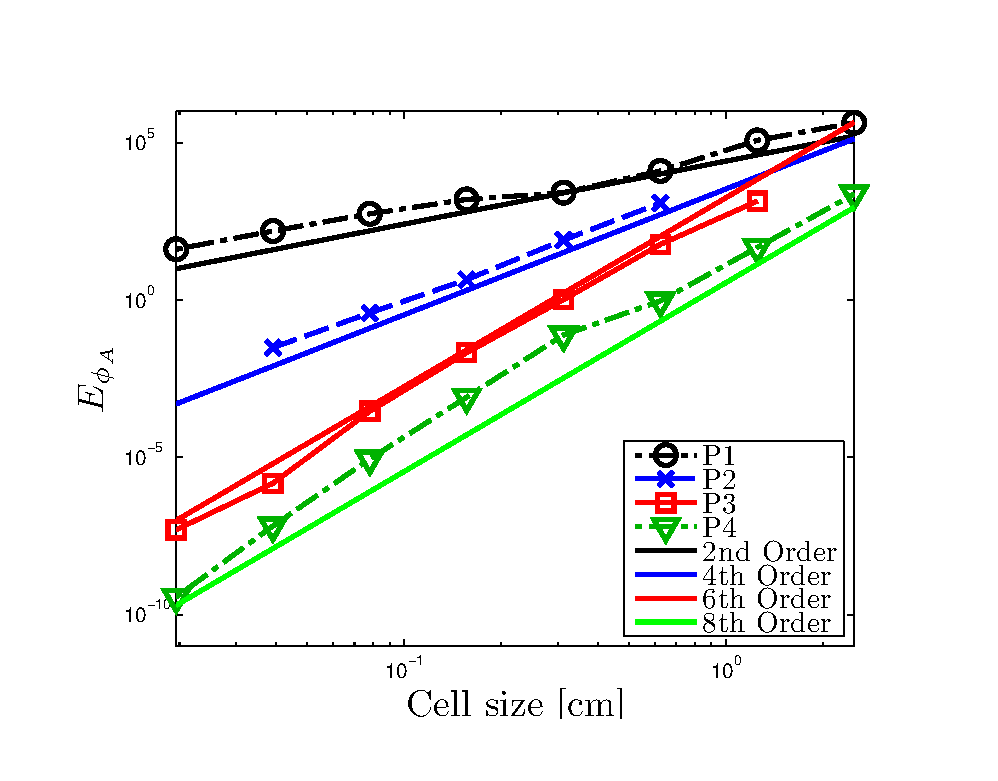
\includegraphics[width=10cm,trim=0.25in  0.2in 0.75in 0.5in,clip=true]{chapter6_grey_radtran/Dissertation_Data/Constant_Time_SLXS_Lobatto_phi_A.pdf}
\caption{Convergence of $E_{\phi_A}$ for SLXS Lobatto scheme, for steady state test problem.}
\label{fig:constant_time_lobatto_phi_a}
\end{figure}
%
%
\begin{figure}[!htp]
\centering
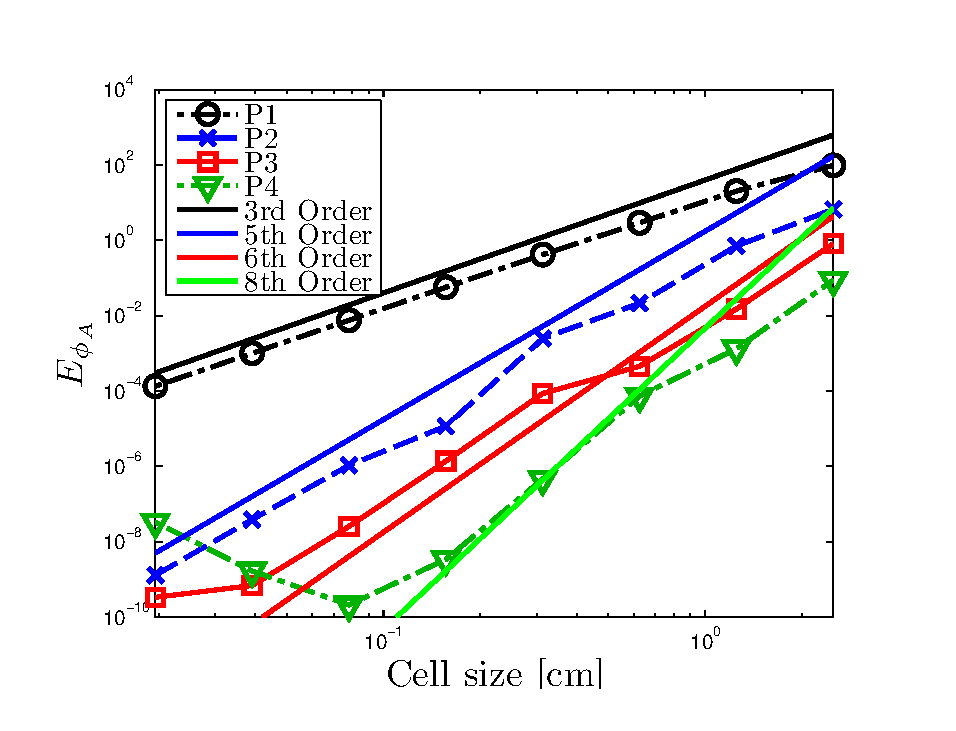
\includegraphics[width=10cm,trim=0.25in  0.2in 0.75in 0.5in,clip=true]{chapter6_grey_radtran/Dissertation_Data/Constant_Time_SLXS_Gauss_phi_A.pdf}
\caption{Convergence of $E_{\phi_A}$ for SLXS Gauss scheme, for steady state test problem.}
\label{fig:constant_time_gauss_phi_a}
\end{figure}

Finally, we consider the convergence of $E_{T_A}$.  
In \fig{fig:constant_time_lobatto_t_a} SLXS Lobatto converges $E_{T_A}$ $\propto 2P$, and in \fig{fig:constant_time_gauss_t_a}
SLXS Gauss converges $E_{T_A} \propto 2P+2$.  
Both of these convergence rates are higher than those observed in any of our previous MMS test problems.
The SLXS Lobatto $E_{T_A}$ convergence rate is equal to the SLXS Lobatto convergence rates for $E_{\psi_A}$ and $E_{IR_A}$, whereas the SLXS Gauss $E_{T_A}$ convergence rate is greater than any convergence rate observed for SLXS Gauss for neutron transport.
\begin{figure}[!htp]
\centering
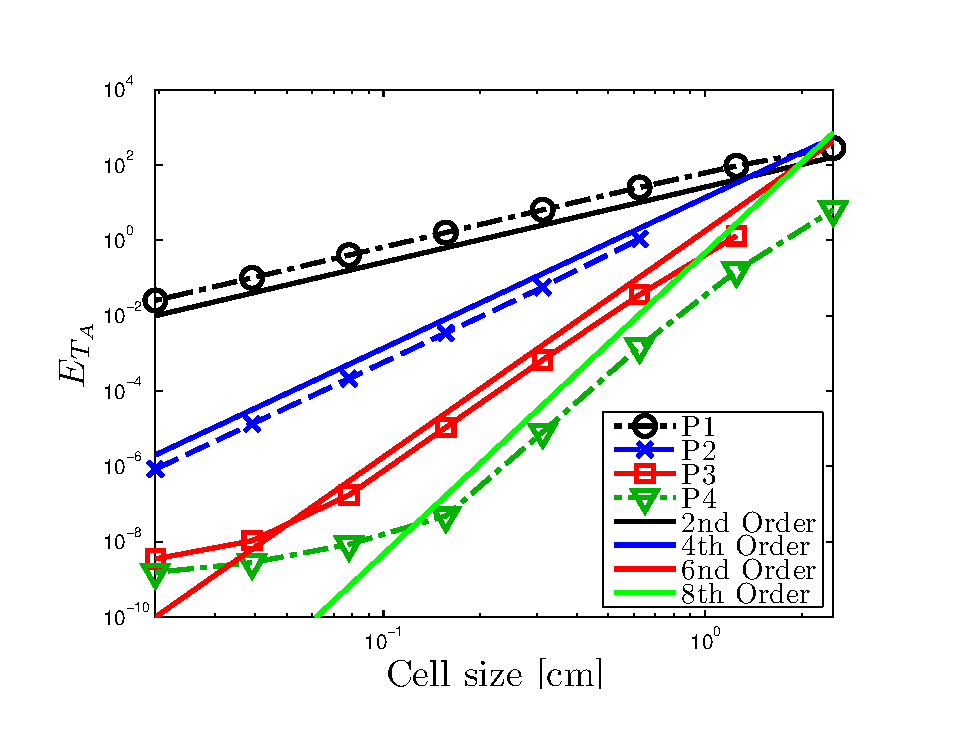
\includegraphics[width=9.5cm,trim=0.25in  0.25in 0.75in 0.5in,clip=true]{chapter6_grey_radtran/Dissertation_Data/Constant_Time_SLXS_Lobatto_temp_A.pdf}
\caption{Convergence of $E_{T_A}$ for SLXS Lobatto scheme, for steady state test problem.}
\label{fig:constant_time_lobatto_t_a}
\end{figure}
%
%
\begin{figure}[!hbp]
\centering
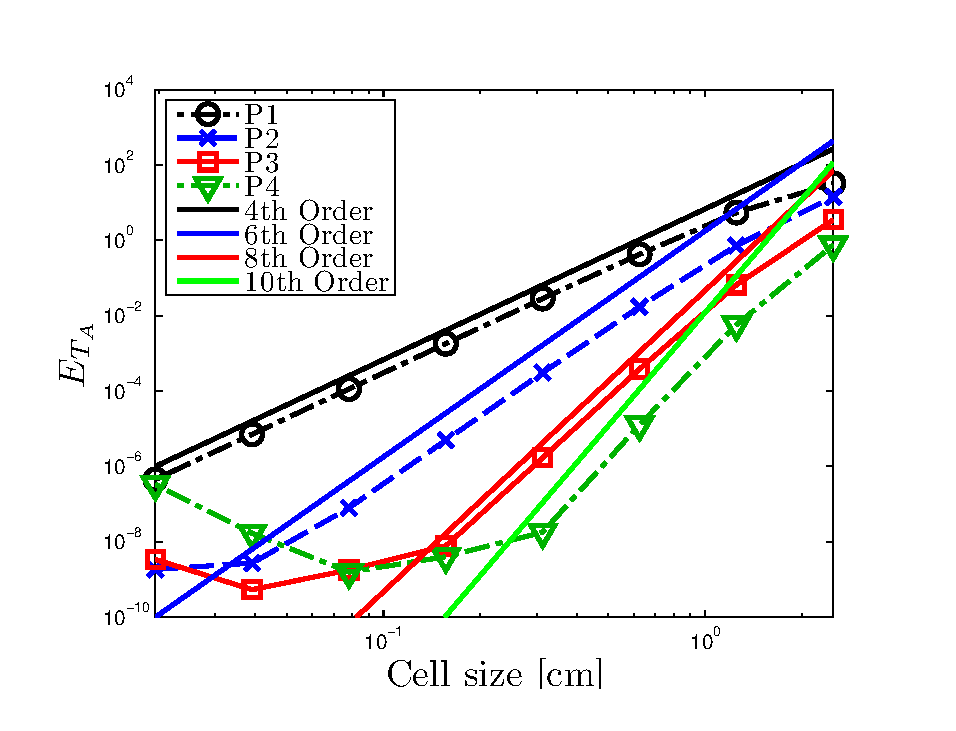
\includegraphics[width=9.5cm,trim=0.25in  0.25in 0.75in 0.5in,clip=true]{chapter6_grey_radtran/Dissertation_Data/Constant_Time_SLXS_Gauss_temp_A.pdf}
\caption{Convergence of $E_{T_A}$ for SLXS Gauss scheme, for steady state test problem.}
\label{fig:constant_time_gauss_t_a}
\end{figure}

%\pagebreak
\newpage
\subsubsection{Constant in Space - Trigonometric in Time}
\label{sec:time_convergence}
We consider three different SDIRK schemes in our work, implicit Euler (IE); a two stage, second order S-stable scheme (2-2); and a three stage, third order S-stable scheme (3-3).
Both multi-stage schemes were taken from \cite{alexander}.
The Butcher tableaux for the implicit Euler scheme can be written as:
\benum
\label{eq:ie}
\begin{array}{c|c|c}
\hline
1						&  1  	& 1	\\
\hline
{}					&				&		1	
\end{array} \pep
\eenum
The 2-2 scheme of Alexander has the following Butcher tableaux,
\benum
\label{eq:alexander_2_2}
\begin{array}{c|c|cc}
\hline
1						&  1-\frac{\sqrt{2}}{2}   &  1-\frac{\sqrt{2}}{2}  	&  0  		\\
2						&  1   &  \frac{\sqrt{2}}{2} & 1-\frac{\sqrt{2}}{2}  	\\	
\hline
{}					&				&		\frac{\sqrt{2}}{2}	&		1- \frac{\sqrt{2}}{2}		
\end{array} \pec
\eenum
and the 3-3 scheme's Butcher tableaux is:
\benum
\label{eq:alexander_3_3}
\begin{array}{c|c|ccc}
\hline
1						&  \gamma   						& \gamma 	&    										&			\\
2						&  \frac{1+\gamma}{2}   &  \frac{1-\gamma}{2} 		& \gamma  	&			\\	
3						&  1   									&   	\delta	& \beta 	 	&		\gamma	\\	
\hline
{}					&												&		\delta		&		\beta			&	\gamma
\end{array} \pec
\eenum
with 
\beanum
\gamma &=& 0.435866521508459 \\
\delta &=& \frac{-6\gamma^2 + 16\gamma -1}{4} \\
\beta &=& \frac{6\gamma^2 - 20\gamma + 5}{4} \pep
\eeanum

We now verify the asymptotic order of convergence of each SDIRK scheme.
To simplify the process, we consider a problem with constant spatial dependence:
\beanum
M(\mu_d) &=& \frac{1}{4\pi} \\
W_I(x) &=& \frac{10}{4\pi} \\
W_T(x) &=&  10 \\
F(t) &=& 45 \cos\left( \pi t \right) + 46 \pec
\eeanum
$t \in[0,1]$, $\sigma_s = 0.1$, $\sigma_a = 2.5$, $C_v = 0.2$, $x\in[0,10]$ discretized with 10 equally spaced cells.  Convergence of $E_{\phi}$ as a function of $\Delta t$ for the IE, 2-2, and 3-3 time differencing schemes is given in \fig{fig:e_phi_time}.
\begin{figure}[!htp]
\centering
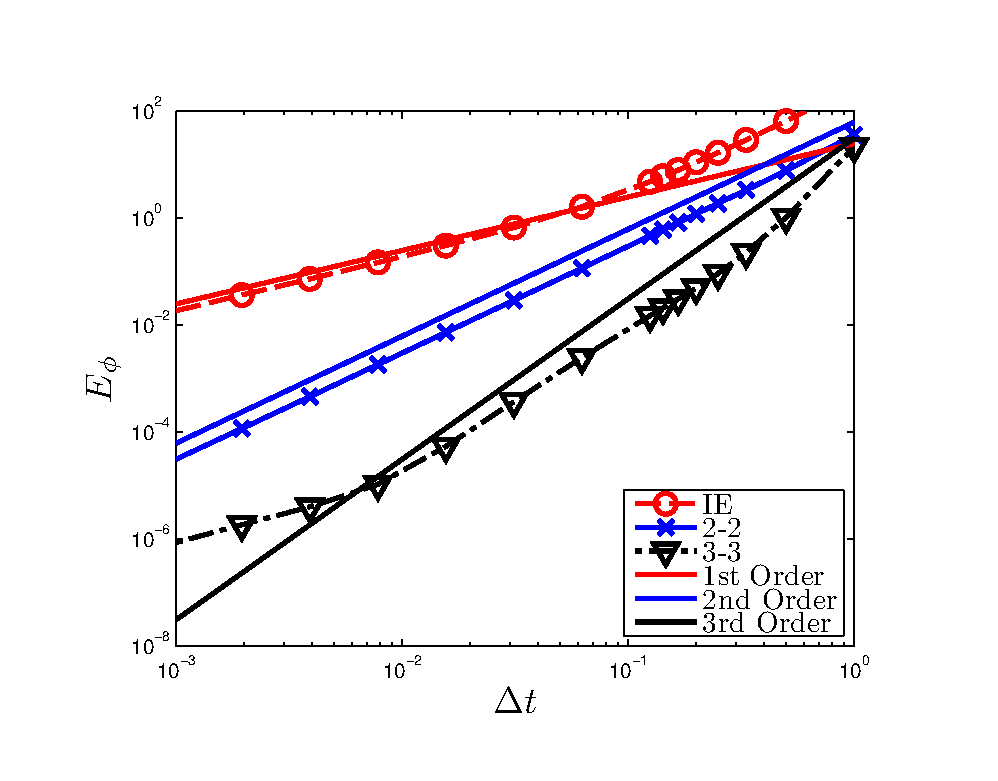
\includegraphics[width=10cm,trim=0.25in  0.2in 0.75in 0.5in,clip=true]{chapter6_grey_radtran/Dissertation_Data/Time_Integrators_Convergence_Phi.pdf}
\caption{Convergence of $E_{\phi}$ for different time integrators as a function of $\Delta t$.}
\label{fig:e_phi_time}
\end{figure}
As expected, the IE converges 1st order in time, the 2-2 scheme converges second order, and the Alexander 3-3 scheme converges third order in time.
The same data for temperature is given in \fig{fig:big_dt}.  
Though the 2-2 and 3-3 schemes are more accurate than IE, it took a very long time for the 2-2 and 3-3 schemes to demonstrate their respective asymptotic orders of convergence for $E_T$ as compared to $E_{\phi}$.
\begin{figure}[!htp]
\centering
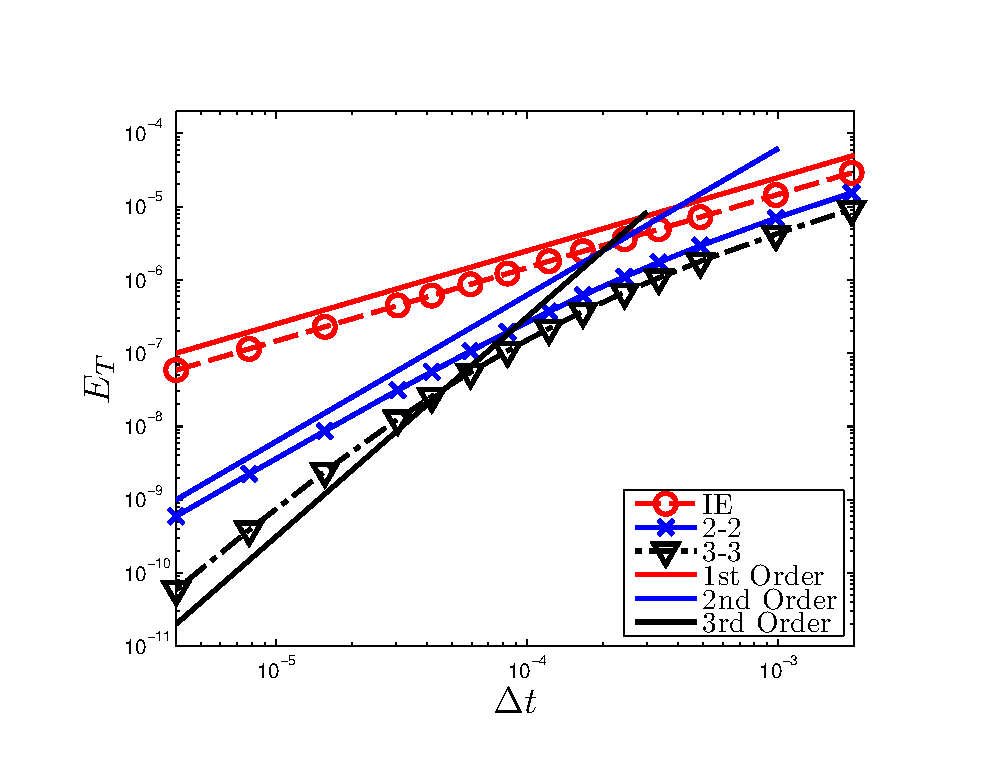
\includegraphics[width=10cm,trim=0.25in  0.2in 0.75in 0.5in,clip=true]{chapter6_grey_radtran/Dissertation_Data/Time_Integrators_Convergence_Temperature.pdf}
\caption{Convergence of $E_{T}$ for different time integrators as a function of $\Delta t$.}
\label{fig:big_dt}
\end{figure}

\subsection{Marshak Wave Problem}

We now consider our most realistic test problem, a Marshak wave test problem.
Originally presented by Ober and Shadid for radiative diffusion \cite{ober_shadid} we compare our $S_2$ solution that uses Gauss quadrature in angle to the solutions presented in \cite{ober_shadid}.
With an $S_2$ Gauss quadrature in angle, the discrete ordinates method is equivalent to a $P_1$ angular discretization in slab geometry \cite{s2sa}.
The radiative diffusion solution of \cite{ober_shadid} could also be considered a $P_0$ approximation.
Thus while not exact, our $P_1$ equivalent solution is nearly equal to the $P_0$ solutions presented in \cite{ober_shadid}.
Like most thermal radiative transfer problems, no analytic solution exists.  
As such, we focus on qualitative comparisons of how DFEM trial space degree, mesh refinement, and time step refinement affect the radiation energy density and material temperature solutions.

The Marshak wave problem consists of an initially cold slab that is heated from the left by an incident radiation intensity, with a vacuum boundary condition on the right.
Again, the problem is dimensionless, $a=c=C_v=1$; $x\in[0,1]$; and we advance the solution from $t=0$ to $t=1$.
Initially, the slab is in thermal equilibrium, and $T=\left( 10^{-5} \right)^{1/4}$.
There is no scattering, $\sigma_s = 0$, and the absorption opacity is temperature dependent, $\sigma_a = \frac{1}{T^3}$.

We use an initial mesh of 20 cells, but also consider results using meshes of 80, 320, and 1280 cells.
Unless otherwise noted, for all simulations we use the 2-2 Alexander scheme.
We begin with a minimum time step of $\Delta t = 5\times 10^{-4}$ and increase the time step size by 10\% until we reach a maximum time step size of $\Delta t = 10^{-2}$.
For our time refinement studies, we divide the minimum and maximum time step sizes both by a factor of 4, 16, or 64.
We consider linear, quadratic, cubic and quartic SLXS Lobatto and SLXS Gauss DFEM schemes.
To demonstrate that assuming a cell-wise constant opacity results in a bladed radiative transfer temperature solution, we also consider linear SL Lobatto with a cell-wise volumetric average opacity.

We first investigate the effect, if any, of assuming a cell-wise constant opacity.  Figure \ref{fig:bladed_rad_profile} shows the linear SL Lobatto radiation energy density solution at $t=1.0$.
Except for the effects of a very coarse spatial mesh when using 20 cells, the radiation energy density solution is effectively smooth, and comparable to the results published in \cite{ober_shadid}.  
The full temperature solution is shown in \fig{fig:bladed_t_profile_full}.
Clearly, the large, non-monotonic discontinuities (blading) observed in the neutron transport interaction rate profile are present in the TRT temperature profile.
In \fig{fig:bladed_t_profile_full}, mesh refinement reduces the magnitude of the temperature solution blading but does not eliminate blading.
To emphasize that blading is not eliminated with mesh refinement, consider \fig{fig:bladed_t_profile_zoom}, that zooms in on the material temperature solution near the Marshak wavefront.
\begin{figure}[!htp]
\centering
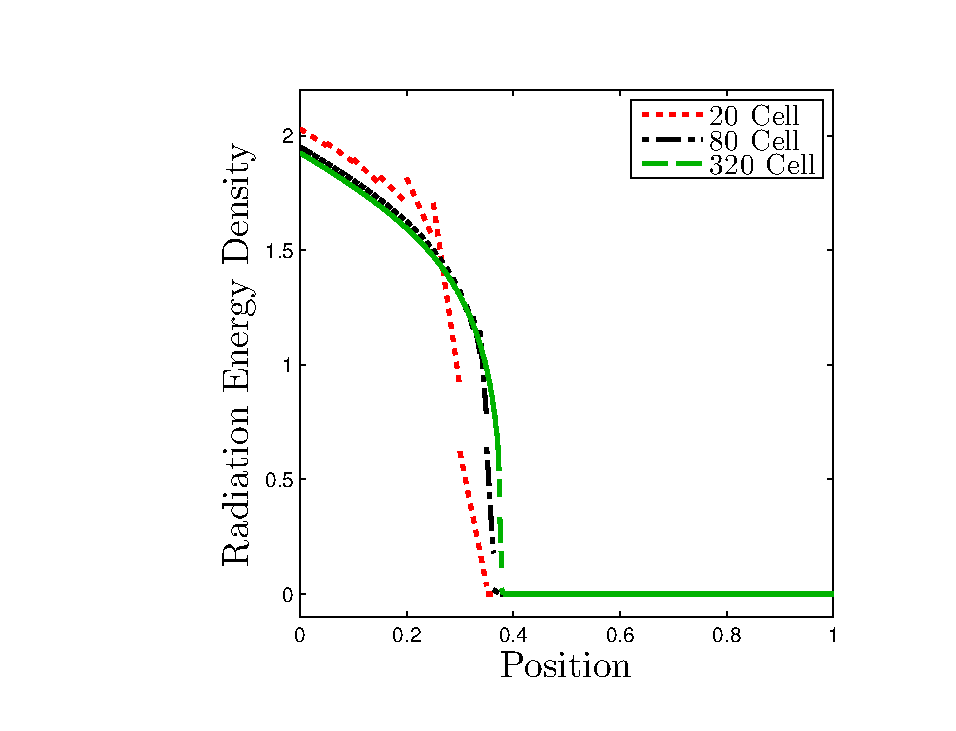
\includegraphics[width=9.5cm,trim=1.2in  0.2in 0.75in 0.5in,clip=true]{chapter6_grey_radtran/Dissertation_Data/Blading_Radiation_Full_MultiCell.pdf}
\caption{Linear SL Lobatto radiation solution for the Marshak wave problem assuming cell-wise constant volumetric averaged opacities.}
\label{fig:bladed_rad_profile}
\end{figure}
%
%
\begin{figure}[!hbp]
\centering
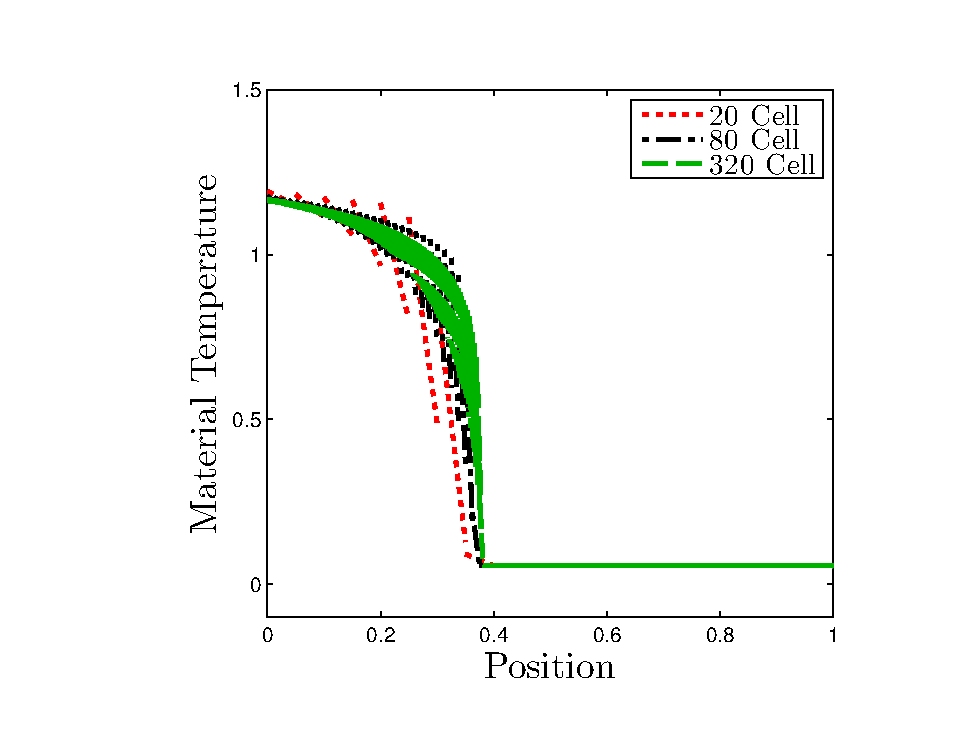
\includegraphics[width=9.5cm,trim=1.2in  0.2in 0.75in 0.5in,clip=true]{chapter6_grey_radtran/Dissertation_Data/Blading_Temperature_Full_MultiCell.pdf}
\caption{Linear SL Lobatto temperature solution for the Marshak wave problem assuming cell-wise constant volumetric averaged opacities.}
\label{fig:bladed_t_profile_full}
\end{figure}
%
%
\begin{figure}[!htp]
\centering
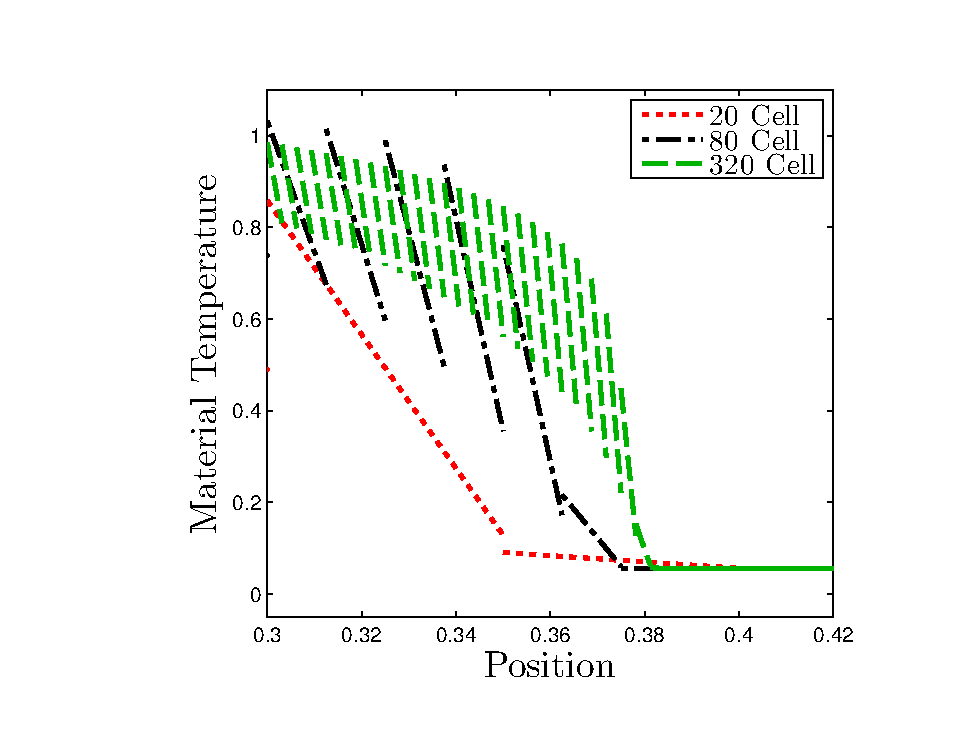
\includegraphics[width=9.5cm,trim=1.2in  0.2in 0.75in 0.5in,clip=true]{chapter6_grey_radtran/Dissertation_Data/Blading_Temperature_Zoom_MultiCell.pdf}
\caption{Linear SL Lobatto temperature solution for the Marshak wave problem near the wavefront.}
\label{fig:bladed_t_profile_zoom}
\end{figure}
Clearly, \figs{fig:bladed_rad_profile}{fig:bladed_t_profile_zoom}, in addition to the limited order of convergence results given \fig{fig:mms3_constant_lobatto_temp} and \fig{fig:mms3_constant_gauss_temp} demonstrate that the assumption of a cell-wise constant opacity is not appropriate for thermal radiative transfer simulations with temperature dependent material properties.

For comparison, consider the linear SLXS Lobatto radiation energy density solution in \fig{fig:linear_slxs_full_rad} and the temperature solution in \fig{fig:linear_slxs_full_temp} using 80 mesh cells.
Visually, there is little difference between the SL Lobatto and SLXS Lobatto angle integrated intensity solutions.
However, this is not the case when examining the material temperature solutions.  Figure \ref{fig:linear_slxs_full_temp} does not exhibit any blading.

%
\begin{figure}[!hbp]
\centering
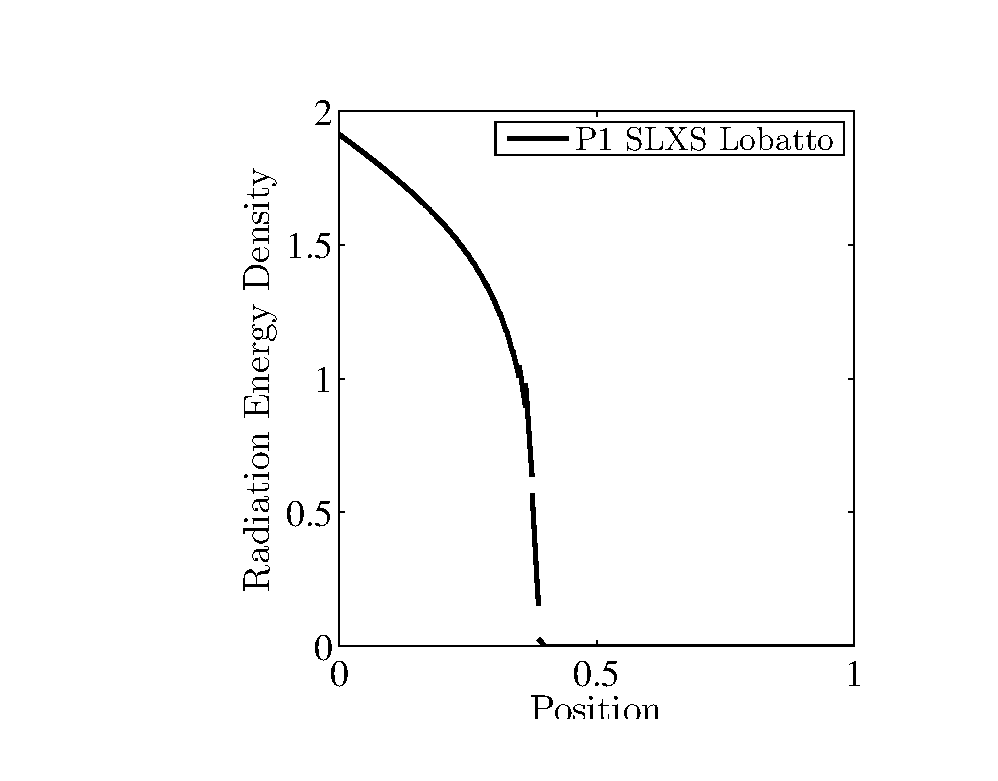
\includegraphics[width=9.5cm,trim=1.2in  0.2in 0.75in 0.5in,clip=true]{chapter6_grey_radtran/Dissertation_Data/SLXS_Lobatto_80_Cells_Radiation.pdf}
\caption{Linear SLXS Lobatto angle integrated intensity solution with 80 cells.}
\label{fig:linear_slxs_full_rad}
\end{figure}
%
%
\begin{figure}[!htp]
\centering
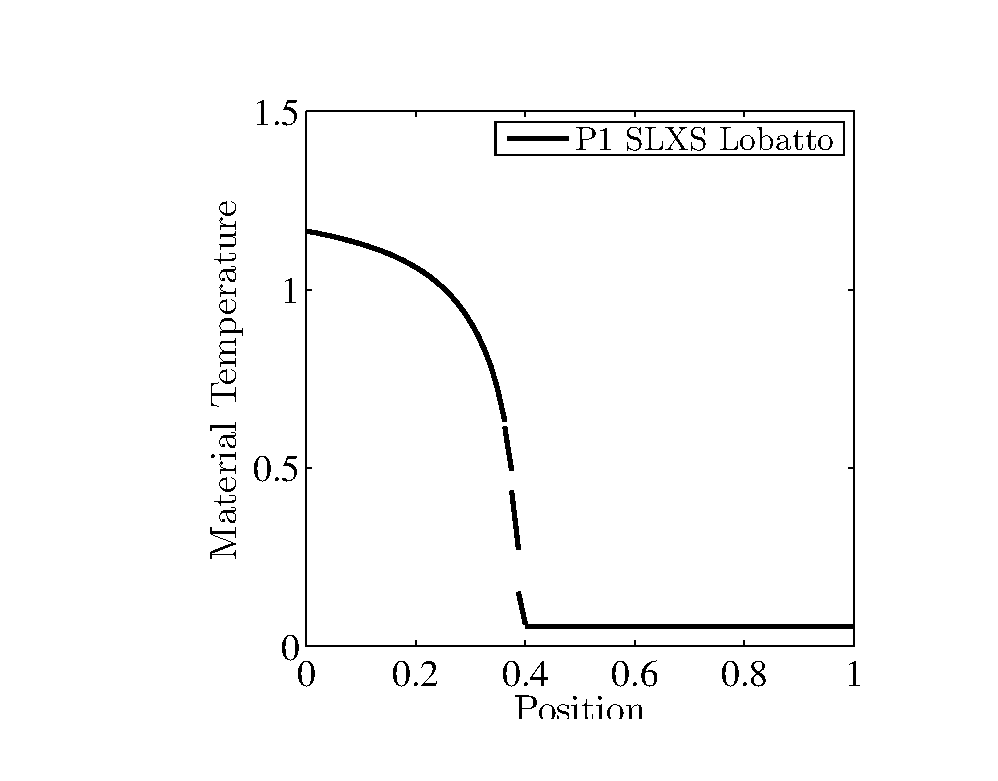
\includegraphics[width=9.5cm,trim=1.2in  0.2in 0.75in 0.5in,clip=true]{chapter6_grey_radtran/Dissertation_Data/SLXS_Lobatto_80_Cells_Temperature.pdf}
\caption{Linear SLXS Lobatto temperature solution with 80 cells.}
\label{fig:linear_slxs_full_temp}
\end{figure}
%

We now consider the effects of spatial mesh refinement on TRT solutions.  
We first consider the linear SLXS Lobatto scheme, looking at a zoom in near the wavefront of the radiation profile in \fig{fig:lobatto_convergence_rad} and the material temperature profile in \fig{fig:lobatto_convergence_temp}
\begin{figure}[!hbp]
\centering
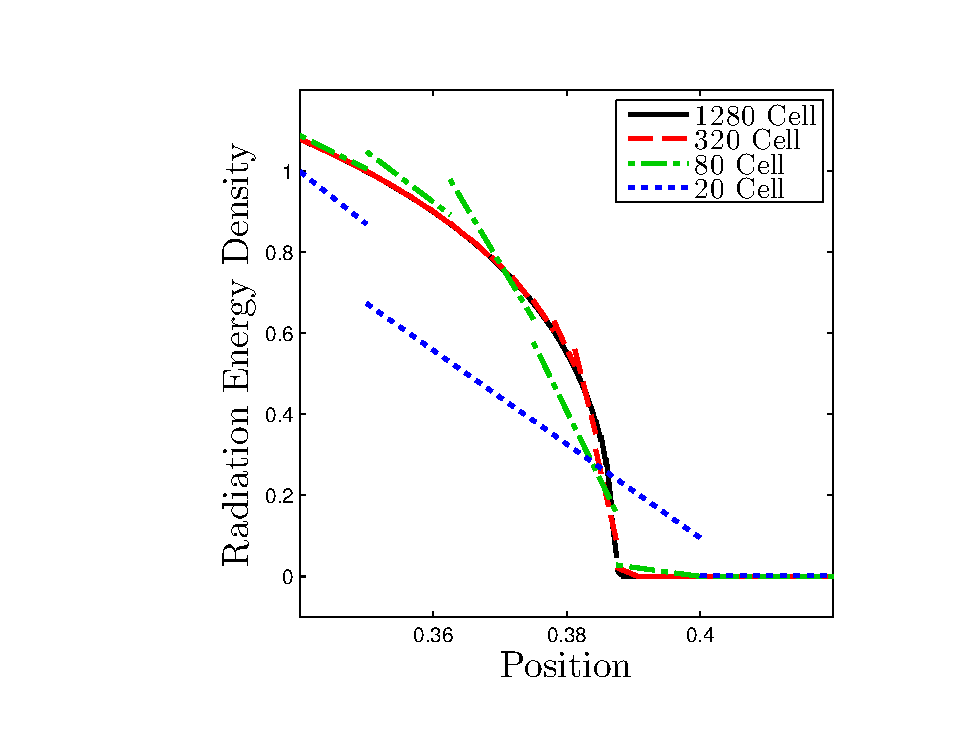
\includegraphics[width=10cm,trim=1.0in  0.2in 0.5in 0.5in,clip=true]{chapter6_grey_radtran/Dissertation_Data/Reorder_Marshak_Zoom_Radiation_SL_Lobatto_P1_Cell_Refinement.pdf}
\caption{Linear SLXS Lobatto radiation solution near wavefront with increasing spatial mesh refinement.}
\label{fig:lobatto_convergence_rad}
\end{figure}
%
%
\begin{figure}[!htp]
\centering
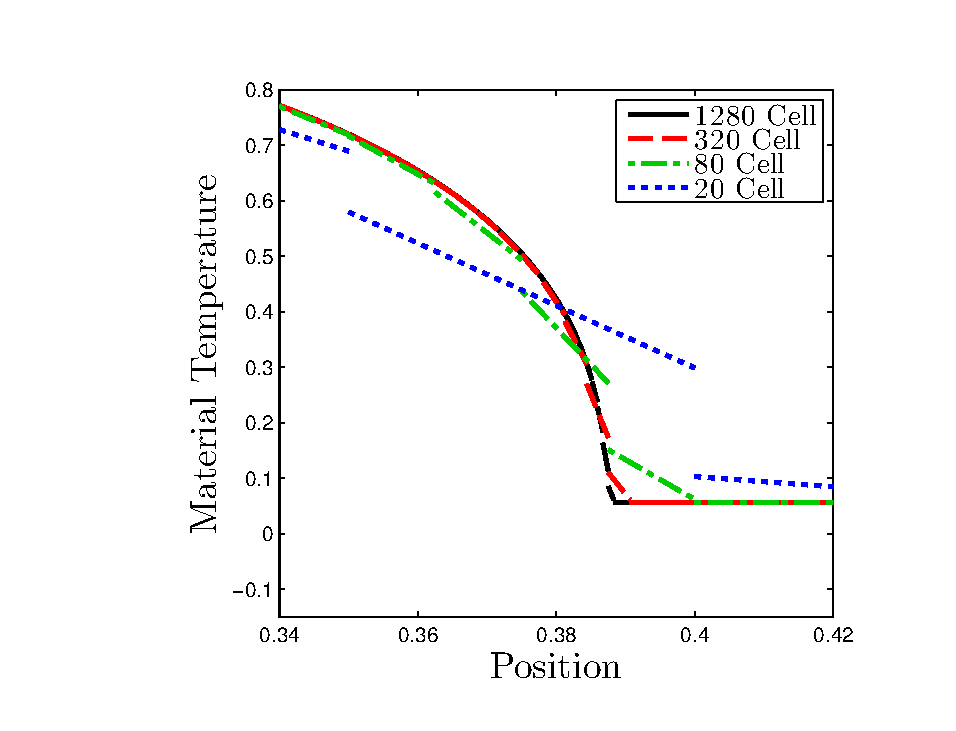
\includegraphics[width=10cm,trim=1.0in  0.2in 0.5in 0.5in,clip=true]{chapter6_grey_radtran/Dissertation_Data/Reorder_Marshak_Zoom_Temperature_SL_Lobatto_P1_Cell_Refinement.pdf}
\caption{Linear SLXS Lobatto temperature solution near wavefront with increasing spatial mesh refinement.}
\label{fig:lobatto_convergence_temp}
\end{figure}
Though the changes are subtle, we can see that mesh refinement actually changes the location of both the radiation and temperature profile discontinuity, with the changes more prominent in the material temperature profile, \fig{fig:lobatto_convergence_temp}.
The changes in the material temperature profile are more pronounced, even when moving from 320 to 1280 mesh cells, than in the radiation profile most likely due to SLXS Lobatto's first order convergence of $E_{T}$.
Plots similar to \fig{fig:lobatto_convergence_rad} and \fig{fig:lobatto_convergence_temp} are provided in \fig{fig:gauss_convergence_rad} and \fig{fig:gauss_convergence_temp}, respectively for the quartic SLXS Gauss scheme.
\begin{figure}[!hbp]
\centering
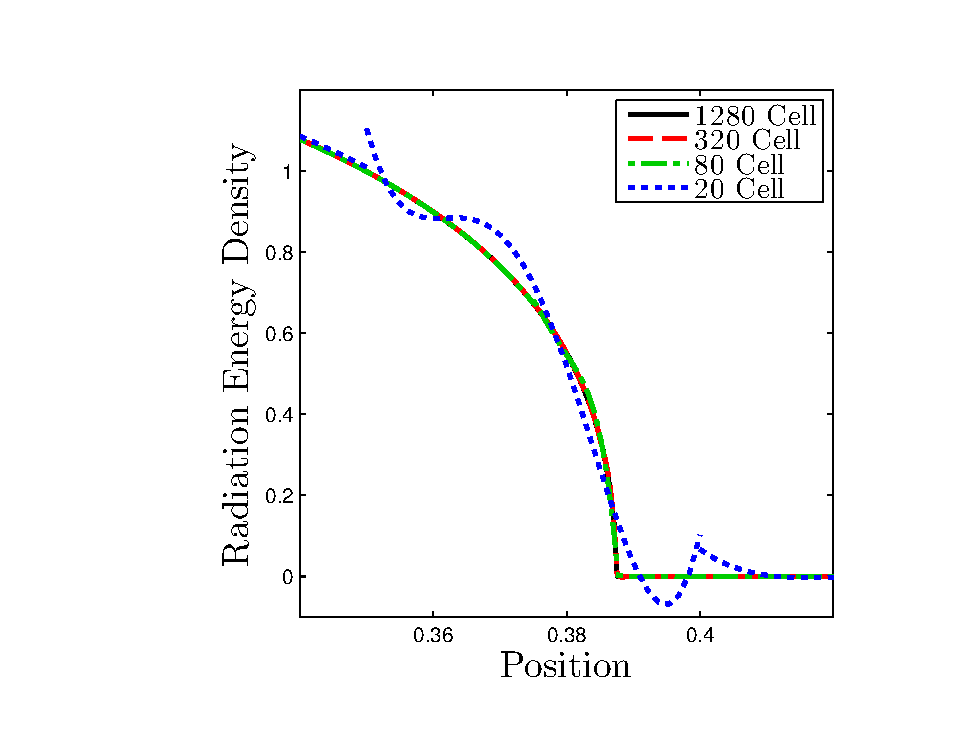
\includegraphics[width=10cm,trim=1.0in  0.2in 0.5in 0.5in,clip=true]{chapter6_grey_radtran/Dissertation_Data/Reorder_Marshak_Zoom_Radiation_SL_Gauss_P4_Cell_Refinement.pdf}
\caption{Quartic SLXS Gauss radiation solution near wavefront with increasing spatial mesh refinement.}
\label{fig:gauss_convergence_rad}
\end{figure}
%
%
\begin{figure}[!htp]
\centering
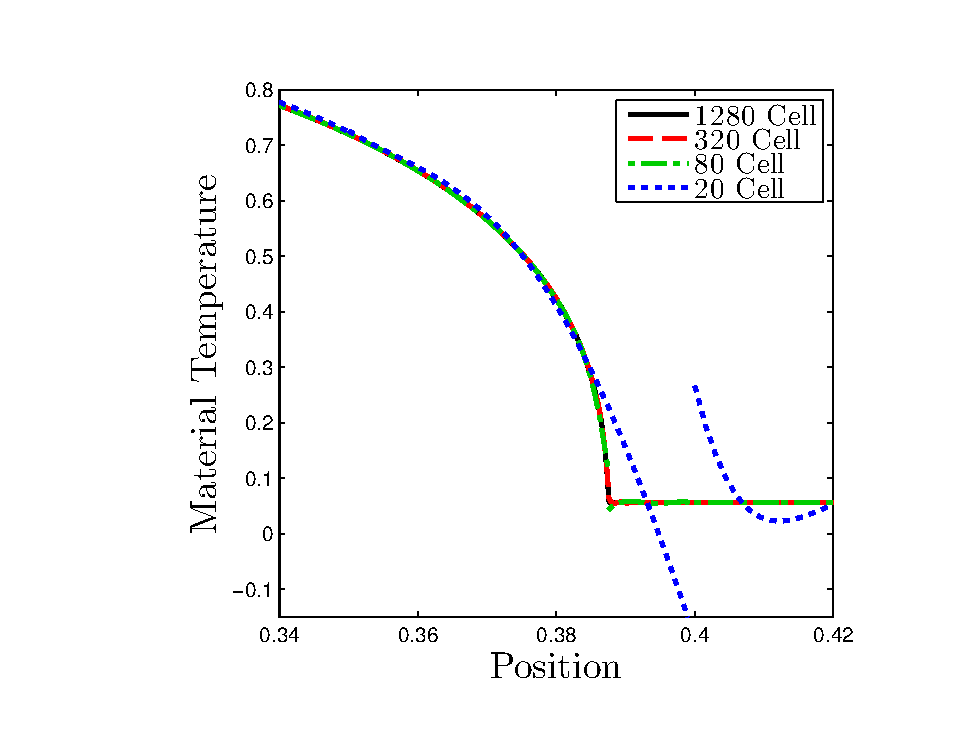
\includegraphics[width=10cm,trim=1.0in  0.2in 0.5in 0.5in,clip=true]{chapter6_grey_radtran/Dissertation_Data/Reorder_Marshak_Zoom_Temperature_SL_Gauss_P4_Cell_Refinement.pdf}
\caption{Quartic SLXS Gauss temperature solution near wavefront with increasing spatial mesh refinement.}
\label{fig:gauss_convergence_temp}
\end{figure}
Due to the SLXS Gauss' high order of spatial convergence, few changes are noticeable with mesh refinement, except when moving from 20 to 80 cells.
However, when moving from 20 to 80 cells, the Gibbs' phenomena near the solution discontinuity are no longer visible, except for a very small negativity in the temperature solution.
All solutions for this spatial mesh refinement study use the finest time step sizes.

We now examine the effect of increasing DFEM trial space degree, on a fixed mesh of 320 spatial cells using SLXS Lobatto, focusing on the region near the Marshak wavefront.
In \fig{fig:p_convergence_rad} we plot the angle integrated intensity profile and plot the temperature profile in \fig{fig:p_convergence_temp}
\begin{figure}[!htp]
\centering
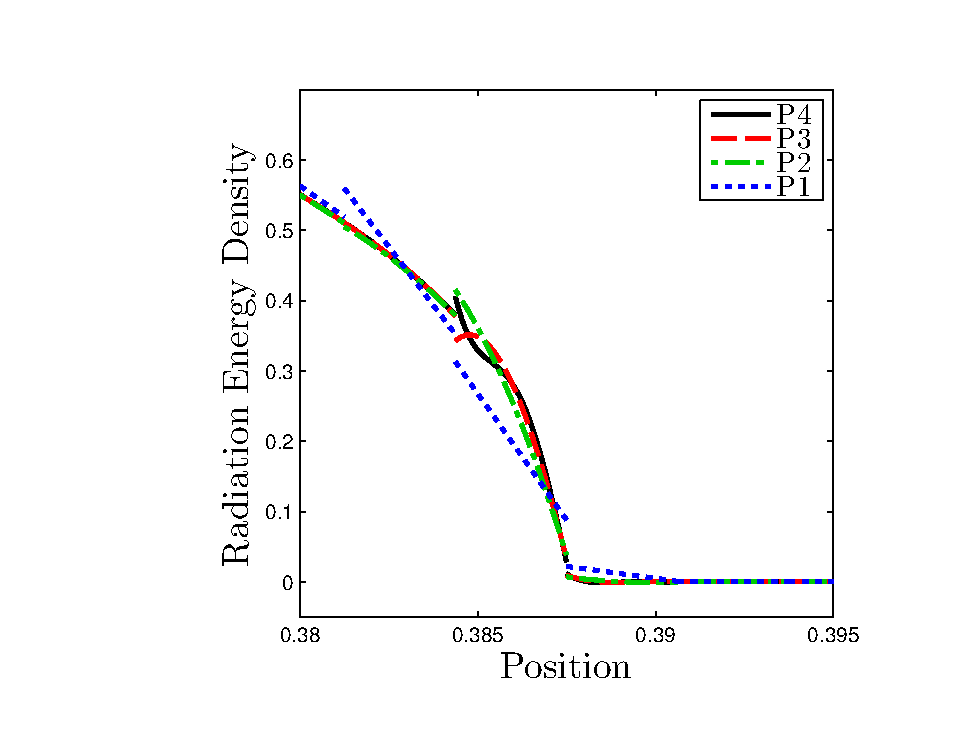
\includegraphics[width=10cm,trim=1.0in  0.2in 0.5in 0.5in,clip=true]{chapter6_grey_radtran/Dissertation_Data/Pointless_Marshak_Zoom_Radiation_Lobatto_P_Refinement.pdf}
\caption{SLXS Lobatto radiation energy density solution with 320 cells for different $P$ near Marshak wavefront.}
\label{fig:p_convergence_rad}
\end{figure}
%
\begin{figure}[!hbp]
\centering
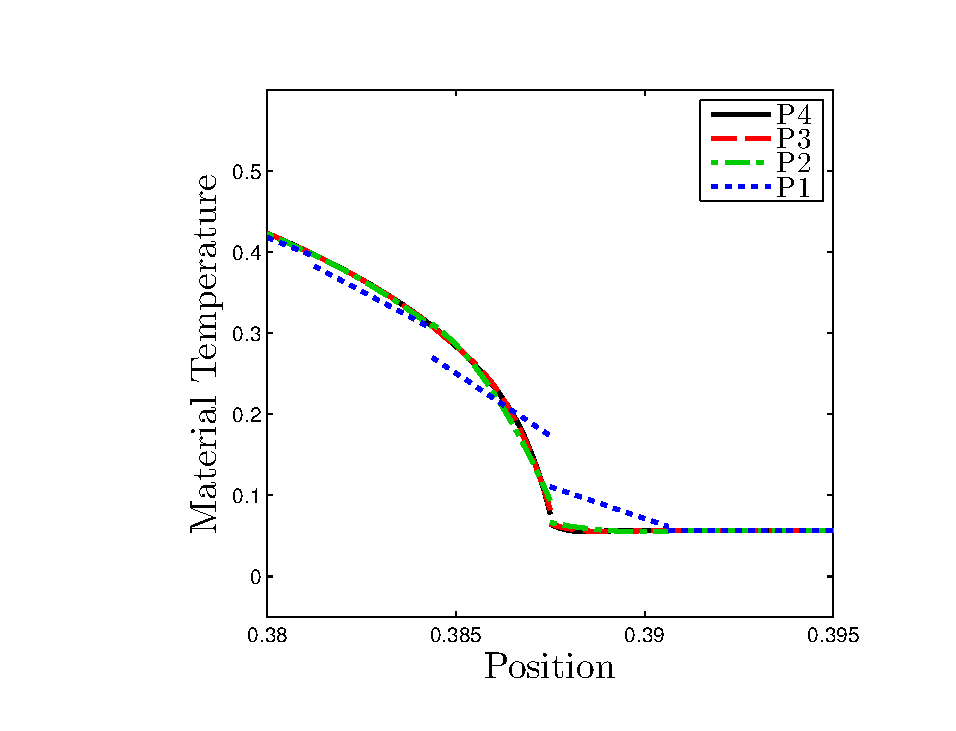
\includegraphics[width=10cm,trim=1.0in  0.2in 0.5in 0.5in,clip=true]{chapter6_grey_radtran/Dissertation_Data/Pointless_Marshak_Zoom_Temperature_Lobatto_P_Refinement.pdf}
\caption{SLXS Lobatto material temperature solution with 320 cells for different $P$ near Marshak wavefront.}
\label{fig:p_convergence_temp}
\end{figure}
Increasing $P$ make the wavefront in the radiation profile sharper, but at a resolution of 320 cells, none of the $P$ considered result in a visually continuous solution.
The most notable changes with increase $P$ come in the temperature profile, where linear SLXS Lobatto does not form a sharp interface, whereas all of the higher $P$ schemes capture the non-smooth transition more accurately.

Before looking at very high spatial resolution solutions, we first consider the effect of time step refinement in \fig{fig:time_refinement_rad} for the radiation profile and in \fig{fig:time_refinement_temp}.
Both \fig{fig:time_refinement_rad} and \fig{fig:time_refinement_temp} use a quartic SLXS Gauss spatial discretization with 1280 cells.
The effects of decreasing time step size are non-trivial near the wavefront.
As seen in \fig{fig:time_refinement_rad}, at lower time resolutions, $\Delta t$ and $\frac{\Delta t}{4}$, the wavefront is visibly not uniform concave down, with several ``wiggles'' in the radiation profile in the heated region of the slab.
Additionally, increased temporal resolution causes the discontinuity at the leading edge of the wavefront to sharpen.
In \fig{fig:time_refinement_temp}, the effects of increased time resolution are the same as in \fig{fig:time_refinement_rad}.
However, increased time resolution more noticeably sharpens the discontinuity in the temperature profile than it eliminates wavefront wiggles, though in \fig{fig:time_refinement_temp} the $\Delta t$ curve is not strictly concave down in the heated region of the slab near the wavefront.
%
%
\begin{figure}[!htp]
\centering
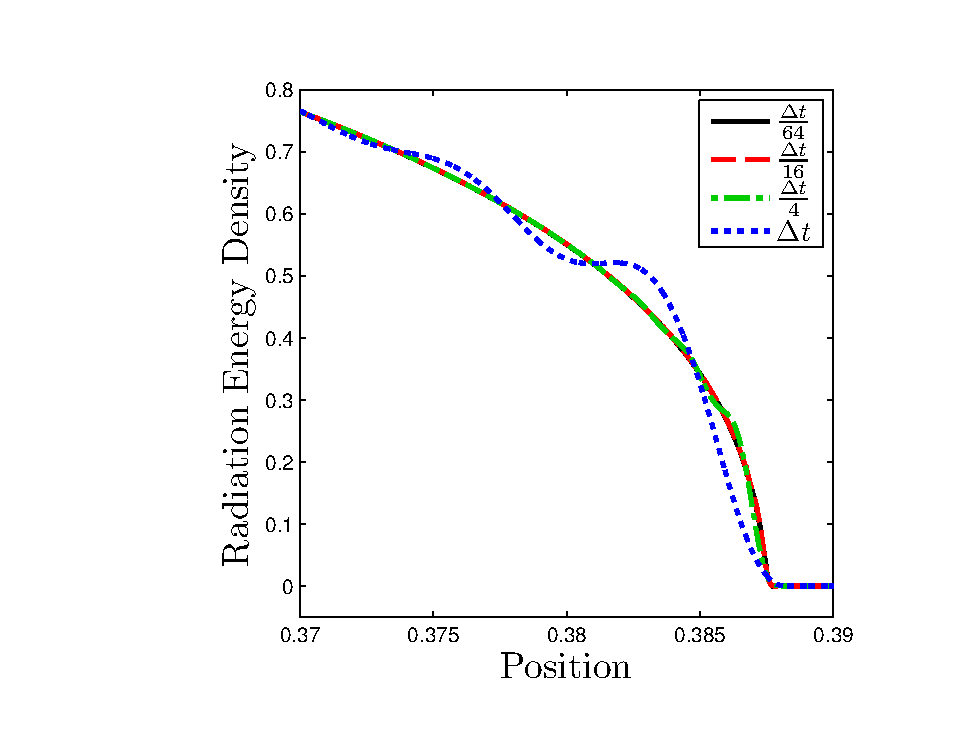
\includegraphics[width=10cm,trim=1.0in  0.2in 0.5in 0.5in,clip=true]{chapter6_grey_radtran/Dissertation_Data/Time_Refinement_Zoom_Radiation.pdf}
\caption{Quartic SLXS Lobatto radiation energy density solution with 1280 cells for different time refinements near the Marshak wavefront.}
\label{fig:time_refinement_rad}
\end{figure}
%
%
\begin{figure}[!hbp]
\centering
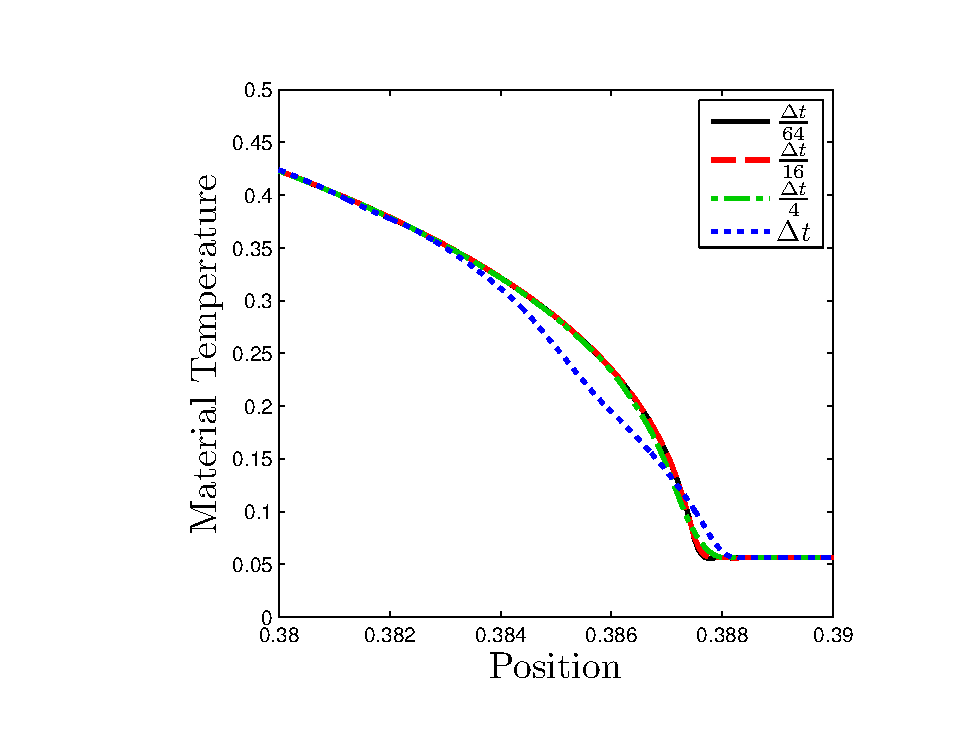
\includegraphics[width=10cm,trim=1.0in  0.2in 0.5in 0.5in,clip=true]{chapter6_grey_radtran/Dissertation_Data/Time_Refinement_Zoom_Temperature.pdf}
\caption{Quartic SLXS Lobatto temperature solution with 1280 cells for different time refinements near the Marshak wavefront.}
\label{fig:time_refinement_temp}
\end{figure}

\pagebreak

We now discuss highly resolved $S_2$ solutions to the Marshak wave problem.
Our hope is that with sufficient spatial resolution and higher order DFEM, we are able to resolve transport boundary layers.
Our highest resolution simulation uses ten thousand spatial mesh cells.
Given the initial, cold temperature of the slab is roughly $T=0.056$,  $\sigma_t = \sigma_a = \frac{1}{T^3}$, then the total slab optical thickness is roughly 5700 MFP thick, and when using ten though cells, each mesh cell is roughly $0.57$ MFP thick.  
As noted by Larsen, Morel, and Miller \cite{thick_diffusion_larsen}, this type of mesh spacing is neither optically thick nor thin.
To answer whether ten thousand mesh cells is sufficient, we first consider \fig{fig:res_zoom_comparison} where we compare the results of cubic SLXS Lobatto schemes that use
\begin{enumerate}
\item ten thousand spatial cells, with ten thousand time steps and the 3-3 SDIRK scheme,
\item ten thousand spatial cells, with one thousand time steps and the 3-3 SDIRK scheme, and 
\item 1280 spatial cells, with six thousand time steps of the 3-3 SDIRK scheme.
\end{enumerate} 
\begin{figure}[!htp]
\centering
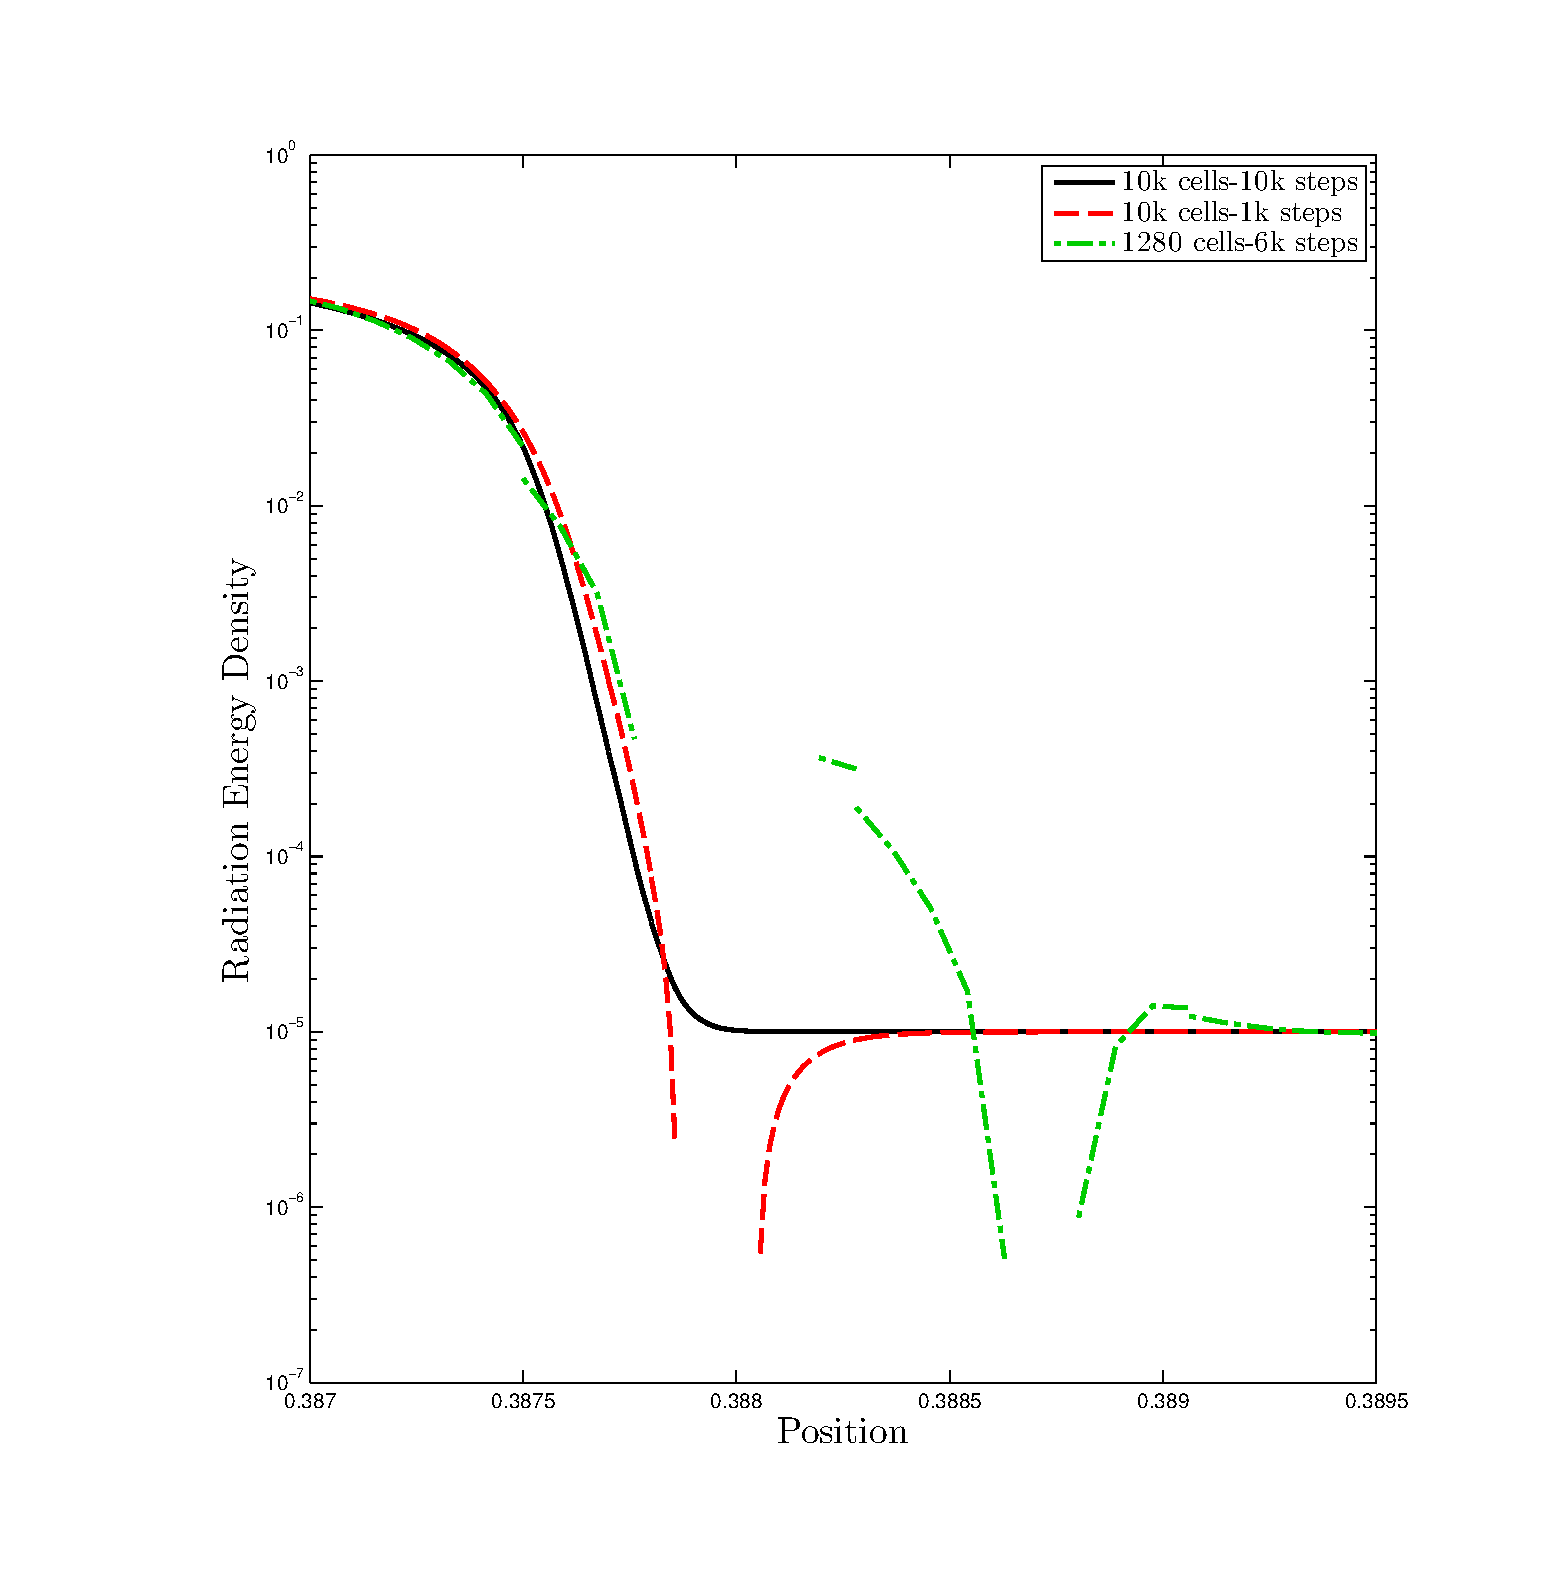
\includegraphics[width=13cm,trim=1.0in  0.75in 1.0in 1.0in,clip=true]{chapter6_grey_radtran/Dissertation_Data/Zoom_10k_Phi.pdf}
\caption{Plot of the radiation energy density on a logarithmic scale for different high resolution simulations near the Marshak wavefront.}
\label{fig:res_zoom_comparison}
\end{figure}
Missing' segments in \fig{fig:res_zoom_comparison} are caused by negative radiation energy densities.
The twelve-hundred cell simulation has only 1 negative node.
The ten thousand cell simulation that uses one thousand time steps has a total of 8 negative nodes; one entire cell has a negative radiation energy density, and two other cells have at least one node with a negative radiation energy density.
Since the ten thousand cell simulation with ten thousand time steps does not have any negative radiation energy densities, it is clear then that temporal resolution is also required.
Unfortunately, noting that the radiation energy density jumps four orders of magnitude for $x\in[0.387 0.388]$, our highest resolution run only had a total of ten cells available to resolve the transport boundary layer.
In \fig{fig:boundary_layer}, we plot the angular intensities for $\mu=\pm\frac{1}{\sqrt{3}}$ of the ten thousand cell, ten thousand time step simulation.  
\begin{figure}[!htp]
\centering
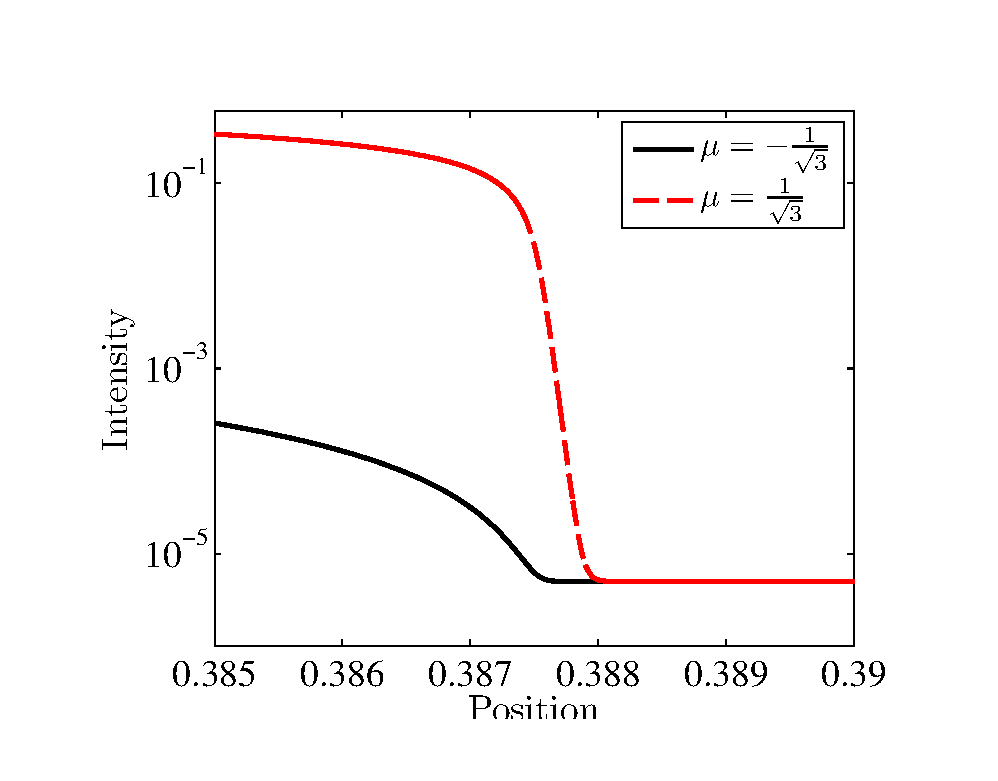
\includegraphics[width=11cm,trim=0.5in  0.0in 0.5in 0.5in,clip=true]{chapter6_grey_radtran/Dissertation_Data/50_Cells_at_Wavefront_Intensity_Log.pdf}
\caption{Plot of the angular intensity on a logarithmic scale near the transport boundary layer at the Marshak wave front.}
\label{fig:boundary_layer}
\end{figure}
Clearly the radiation traveling from the hot to cold region, $\mu=\frac{1}{\sqrt{3}}$ has the largest boundary layer, but even with less than ideal spatial resolution, the rapid rise in angular intensity appears to be smooth, suggesting we have resolved the radiation boundary layer.

Finally, we consider higher $S_N$ solutions to the Marshak wave problem.  First, we compare the $S_8$ solution to the $S_2$ solution for material temperature in \fig{fig:s2_vs_s8_temperature} and for radiation energy density in \fig{fig:s2_vs_s8_radiation}.  The $S_8$ solution in \figs{fig:s2_vs_s8_temperature}{fig:s2_vs_s8_radiation} was generated using quartic SLXS Gauss with five thousand spatial cells, the Alexander 2-2 SDIRK scheme and approximately ten thousand time steps.
\begin{figure}[!htp]
\centering
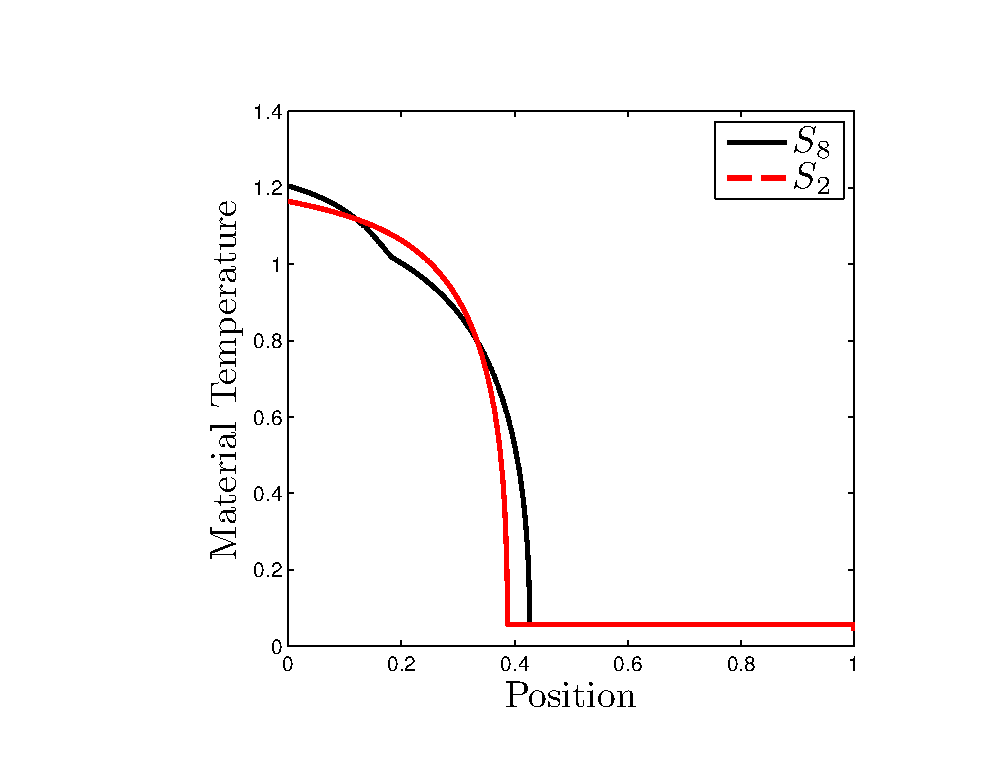
\includegraphics[width=11cm,trim=1.0in  0.5in 0.2in 0.6in,clip=true]{chapter6_grey_radtran/S8_vs_S2_Material_Temperature.pdf}
\caption{$S_8$ and $S_2$ material temperature profiles.}
\label{fig:s2_vs_s8_temperature}
\end{figure}
%
\begin{figure}[!htp]
\centering
\includegraphics[width=11cm,trim=1.0in  0.3in 0.2in 0.5in,clip=true]{chapter6_grey_radtran/S8_vs_S2_Radiation_Energy_Density.pdf}
\caption{$S_8$ and $S_2$ radiation energy density profiles.}
\label{fig:s2_vs_s8_radiation}
\end{figure}
The $S_8$ solution exhibits many of the qualitative features we would expect a transport solution to exhibit versus the $S_2$ solution which is very close to the diffusion solution.
For example, we expect the transport solution to have a higher temperature solution near the problem boundary, with a more rapid drop in both the material temperature and radiation energy density/angle integrated intensity solutions relative to a diffusion solution.
Additionally, we expect the transport material temperature and radiation energy density solution to penetrate farther into the slab than the diffusion solution, but with a less steep gradient.
Figures \ref{fig:s2_vs_s8_radiation}-\ref{fig:s2_vs_s8_temperature} both exhibit this behavior, caused by the transport solution becoming more and more like $\delta(\mu-1)$ in optically thick regions. 
However, we did not expect the non-smooth features near $x=0.2$.
We suspect this is caused by the rapid attenuation of the most glancing $\mu$ from the incident boundary conditions.
To verify this, we plot the $S_8$ intensity solution in \fig{fig:s8_intensity_full}.
\begin{figure}[!htp]
\centering
\includegraphics[width=16cm,trim=1.5in  0.5in 0.2in 1in,clip=true]{chapter6_grey_radtran/S8_Intensity_SemiLogy.pdf}
\caption{Log plot of $S_8$ intensities for Marshak wave problem.}
\label{fig:s8_intensity_full}
\end{figure}

We now zoom in to the boundary layer intensities near $x=0.2$ and near the thermal wave front.
In \fig{fig:s8_zoom_glance}, it is clear that the intensity in the direction of $\mu=+0.1834$ experiences a rapid variation as the incident flux from the boundary is rapidly attenuated, and the isotropic emission from the heated regions of the slabs becomes the main contributor to $I(\mu_d = +0.1834)$.
It is also clear that despite having 25 cells with quartic DFEM in the region $x\in[.18,.185]$, the factor $\approx 7\times$ step drop in $I(\mu_d = +0.1834)$ cannot be fully resolved. 
\begin{figure}[!ht]
\centering
\includegraphics[width=12cm,trim=0.5in  0.2in 0.5in 0.5in,clip=true]{chapter6_grey_radtran/Dissertation_Data/S8_pos_mu_glance_boundary_layer_log.pdf}
\caption{Logarithmic plot of intensity near glancing $\mu=+0.1834$ boundary layer. }
\label{fig:s8_zoom_glance}
\end{figure}

Near the hot/cold material interface, all but the most glancing $\mu_d > 0$ experience a rapid variation (greater than a factor of 1000 reduction) in angular intensity.
The more glancing $\mu_d$, the sooner the transition, relative to the left boundary.
Given the smooth, profiles for $\mu_d > 0.2$, it also appears that we are able to fully resolve these boundary layers. 
\begin{figure}[!ht]
\centering
\includegraphics[width=16cm,trim=1.5in  0.2in 0.5in 0.75in,clip=true]{chapter6_grey_radtran/Dissertation_Data/S8_thermal_wavefront_boundary_layer.pdf}
\caption{Logarithmic plot of intensity boundary layers near thermal wavefront.}
\label{fig:s8_zoom_thermal_wavefront}
\end{figure}

Our final look at the Marshak wave problem investigates the structure of an $S_{32}$ solution with 1000 spatial cells, quartic SLXS Gauss, and five thousand time steps using the 2-2 time integration scheme.
The material temperature solution is plotted in \fig{fig:s8_vs_s32_temperature} against the $S_8$ solution that uses quartic SLXS Gauss,  five thousand spatial cells, and ten thousand 2-2 time integration steps.
Likewise, the angle integrated intensity solutions are compared in \fig{fig:s8_vs_s32_radiation}.
\begin{figure}[!htp]
\centering
\includegraphics[width=16cm,trim=1.5in  0.2in 0.5in 0.75in,clip=true]{chapter6_grey_radtran/Dissertation_Data/S8_vs_S32_Material_Temperature.pdf}
\caption{Comparison of $S_8$ and $S_{32}$ material temperature profiles for Marshak wave problem.}
\label{fig:s8_vs_s32_temperature}
\end{figure}
%
%
\begin{figure}[!htp]
\centering
\includegraphics[width=16cm,trim=1.5in  0.2in 0.5in 0.75in,clip=true]{chapter6_grey_radtran/Dissertation_Data/S8_vs_S32_Radiation.pdf}
\caption{Comparison of $S_8$ and $S_{32}$ angle integrated intensity solutions for Marshak wave problem.}
\label{fig:s8_vs_s32_radiation}
\end{figure}
Even with $S_{32}$ Gauss quadrature, we continue to see non-smooth dips in both the material temperature and angle integrated intensity profiles, however the dips are significantly smaller for the $S_{32}$ solution as compared to the $S_8$ solution, particularly for the material temperature profile.
In \fig{fig:s8_vs_s32_radiation}, we no longer observe one dip in the angle integrated intensity profile, but rather four smaller dips.
Suspecting these are caused by glancing incidence angles in the quadrature set, we plot the angular intensity for all $\mu_d > 0$ in \fig{fig:s32_intensity}.
\begin{figure}[!htp]
\centering
\includegraphics[width=16cm,trim=1.5in  0.2in 0.5in 0.75in,clip=true]{chapter6_grey_radtran/Dissertation_Data/S32_Intensity.pdf}
\caption{$S_{32}$ intensity solutions for all $\mu_d > 0$, for the Marshak wave problem.}
\label{fig:s32_intensity}
\end{figure}
As with the $S_8$ solution, the dips in $\phi$ are associated with corresponding dips in $I_d$ for glancing $\mu_d>0$.\
The discontinuity associated with $\mu_d = 0.3319$ is obscured in \fig{fig:s8_vs_s32_radiation} as the dip occurs just as the $S_{32}$ angle integrated intensity cross over the $S_8$ angle integrated intensity solution.
The $\mu_d=0.0483$ intensity jump in \fig{fig:s32_intensity} causes the greatest effect in \fig{fig:s8_vs_s32_radiation} for two reasons.  
First, the most glancing quadrature angle is attenuated the most rapidly and as such would be expected to have the greatest drop in value.
Second, Gauss angular quadrature assigns the greatest weight to the quadrature points most near $\mu_d = 0$. 
Thus even if every discrete ordinate intensity had the same decrease in $I$, the jump in $\phi$ would be largest only for the most glancing $\mu$, $\mu=0.0483$.
Surprisingly, the $S_8$ and $S_{32}$ calculations have nearly identical positions and values of the temperature and angle integrated intensity solution near the problem boundary and the hot/cold interface.  
If however, the goal is a smooth transport solution, the value of $N$ required to create a smooth $S_N$ $\phi$ solution appears to be much higher than $S_{32}$.

\subsection{Su-Olson Problem}

The Su-Olson problem \cite{su_olson_1} is an analytic benchmark that consists of an initially cold (initial radiation energy density and temperature conditions are identically absolute zero) half-space slab, heated for a finite amount of time by a volumetric, isotropic radiation source.
The slab's scattering opacity is constant in space and temperature, absorption opacity is constant in space and temperature, and $C_v \propto T^3$.
Assuming $C_v = \alpha T^3$ is critical; as Long, et al. \cite{alex_paper} noted, the assumption regarding $C_v$ is not physical, but is required to make the thermal radiative transfer equations linear in $I$ and $T^4$, or conversely linear in $I$ and material energy density. 
After a series of transformations, Su and Olson derived an analytic solution to the thermal radiative transfer equations under these conditions; their solution is more accurately described as being semi-analytic.
While the radiation energy density and material temperature at every point can be expressed as a closed form integral, evaluation of each integral requires numerical estimation.
Further, the integral is a 2-D, indefinite integral (in both variables) of a trigonometric function with a slowly  decaying exponential argument.
However, \cite{su_olson_1} provides several radiation energy density and material energy density points in space, and thus the Su-Olson problem is beneficial as a benchmark problem to verify the physics of a given radiative transfer implementation.

Given the initial temperature condition is explicitly zero, this implies the initial $C_v$ is also zero.
This is problematic when solving explicitly for temperature and not material energy.
A near-zero heat capacity would result in the material rapidly heating, but a zero heat capacity implies a material that cannot accept heat, and thus can never be heated up.
To prevent this problem, we modify the definition of $C_v$:
\benum
C_v = 10^{-8} + \alpha T^3 \pep
\eenum
Alternatively, we could set an initial temperature to be a non absolute zero value.

Since \cite{su_olson_1} presents results in a non-dimensional format, we elect to define $a=c=1$, $\sigma_a = 1$, $\sigma_s=0$, $\alpha = 4$, truncate the full half space to $x\in[0,5]$, and define the reference temperature, $T_H = 1$.
We solve the problem using 200 spatial mesh cells, linear SLXS Lobatto DFEM, the Alexander 2-2 time differencing scheme, an initial time step size of $\Delta t = 10^{-5}$, and increase the time step size by a factor of 1.1 until a maximum time step size of $\Delta t = 10^{-3}$ is reached.

In \fig{fig:su_olson_s2_rad} we present the radiation energy density solution, $W(x)$ (in the notation on \cite{su_olson_1}), for $S_2$ angular differencing plotted against the analytic diffusion and transport solutions.  Likewise, in \fig{fig:su_olson_s2_mat}, we plot the material energy density, $V(x)$ (in the notation on \cite{su_olson_1}) for $S_2$ angular differencing.
Solutions at various times, $\tau = 1$ and $\tau=10$ are given in both plots.
As expected, the $S_2$ solution is nearly identical to diffusion, but skews slightly in the direction of the full transport solution.
\begin{figure}[!htp]
\centering
\includegraphics[width=8cm,trim=1.75in  0.5in 0.75in 0.5in,clip=true]{chapter6_grey_radtran/Dissertation_Data/Su_Olson_S2_Radiation_Energy.pdf}
\caption{$S_2$ radiation energy density profile for Su-Olson problem.}
\label{fig:su_olson_s2_rad}
\end{figure}
\begin{figure}[!hbp]
\centering
\includegraphics[width=8cm,trim=1.75in  0.5in 0.75in 0.5in,clip=true]{chapter6_grey_radtran/Dissertation_Data/Su_Olson_S2_Material_Energy.pdf}
\caption{$S_2$ material energy density profile for Su-Olson problem.}
\label{fig:su_olson_s2_mat}
\end{figure}

Increasing the number of discrete ordinates, the radiation energy density profile and material energy density profiles are given in \fig{fig:su_olson_s8_rad} and \fig{fig:su_olson_s8_mat} for $S_8$ angular differencing.
\begin{figure}[!htp]
\centering
\includegraphics[width=8cm,trim=1.75in  0.5in 0.75in 0.5in,clip=true]{chapter6_grey_radtran/Dissertation_Data/Su_Olson_S8_Radiation_Energy.pdf}
\caption{$S_8$ radiation energy density profile for Su-Olson problem.}
\label{fig:su_olson_s8_rad}
\end{figure}
\begin{figure}[!hbp]
\centering
\includegraphics[width=8cm,trim=1.75in  0.5in 0.75in 0.5in,clip=true]{chapter6_grey_radtran/Dissertation_Data/Su_Olson_S8_Material_Energy.pdf}
\caption{$S_8$ material energy density profile for Su-Olson problem.}
\label{fig:su_olson_s8_mat}
\end{figure}
By adding a few discrete directions to the quadrature set, our numerical solution becomes indistinguishable from published results of \cite{su_olson_1}, and we conclude that our TRT equation implementation is valid.

\subsection{Effectiveness of MIP DSA for Radiative Transfer}

As of yet, we have failed to have any discussion of the iterative performance of MIP DSA applied to the grey thermal radiative transfer equations.
Though the problems we have considered are not necessarily optically thick, we have used MIP DSA to solve all problems.
A large number of the problems we have considered are not optically thick, in part because we were interested in spatial error convergence.
In \tbl{tbl:iteration_count}, we give a sampling of the average number of iterations required to update the intensity for a given thermal iteration for the problems we have considered thus far.

Several observations can be made regarding the data in \tbl{tbl:iteration_count}.  
Most importantly, MIP DSA applied to the grey TRT is a stable iterative scheme and at worst requires as many iterations as source iteration alone.
Also, the number of iterations for MIP DSA and SI are nearly equal only for most of the problems we have considered, but for those where SI requires larger number of iterations, the ratio of SI+DSA iterations to SI alone iterations grows.
Finally, MIP DSA is compatible with the self-lumping DFEM schemes we have developed that explicitly account for the within cell variation of opacity and heat capacity.

\begin{table}[!htp]
\centering
\caption{Iteration count for different TRT model problems.}
\begin{tabular}{|c|c|c|c|}
\hline
Problem Description & Scheme & Average DSA+SI & Average SI \\
{}									&				 &  Iterations & Iterations  \\
\hline
MMS Constant Time & Linear  & 1.4 & 2.4 \\
4 cells 					& SLXS Lobatto & {} & {} \\
\hline
MMS Constant Time	 & Cubic 			 & 1.6 & 2.3 \\
8 cells 						& SLXS Lobatto & {} & {} \\
\hline
MMS Constant Time	 & Cubic 				 & 1.8 & 1.8 \\
128 cells 					& SLXS Lobatto & {} & {} \\
\hline
MMS1 						& Quadratic 		& 2.0 & 13.5 \\
2 cells 				& SLXS Gauss 		& {}  & {} \\
\hline
MMS1 						& Quadratic 	& 3.0 & 13.6 \\
32 cells 				& SLXS Gauss 	& {} & {} \\
\hline
MMS1	 				& Quadratic  & 4.0 & 13.5 \\
128 cells 		& SLXS Gauss & {} & {} \\
\hline
MMS1 					& Quadratic		& 4.2 & 13.5 \\
256 cells 		& SLXS Gauss 	& {} & {} \\
\hline
MMS2 						& Linear	 & 1.0 & 2.7 \\
2 cells 					& SLXS Gauss & {} & {} \\
\hline
MMS Constant Space 									& Quartic 				 & 17.0 & 39.0 \\
Alexander 3-3, $\Delta t=1$					& SLXS Lobatto 			& {}  & {} \\
\hline
MMS Constant Space 										& Quartic 				 & 6.6 & 11.7 \\
Alexander 3-3, $\Delta t=\frac{1}{8}$	& SLXS Lobatto 			& {}  & {} \\
\hline
MMS Constant Space 										& Quartic 				 & 2.3 & 4.9 \\
Alexander 3-3, $\Delta t=\frac{1}{128}$	& SLXS Lobatto 			& {}  & {} \\
\hline
Marshak Wave 									&  Linear			 & 2.1 & 2.9 \\
20 cells, largest $\Delta t$	& SLXS Lobatto & {} 		 & {} \\
\hline
\end{tabular}
\label{tbl:iteration_count}
\end{table}

To demonstrate the iterative effectiveness of MIP DSA we now present a problem designed solely to be optically thick.
We again define a dimensionless problem, $a=c=1$.
We assume a constant $C_v = 0.05$, define $x\in[0,100]$, $t\in[0,5]$, $\sigma_s = 0$, and $\sigma_a = \frac{5000}{T^2}$.
Initially, the slab is in thermodynamic equilibrium at a temperature of $T=0.5$, and is heated with an incident current of $100$ on the left hand side of the slab.
We difference the problem with linear SLXS Lobatto using 50 spatial cells, implicit Euler in time differencing, and a maximum time step size of $\Delta t_{max} = 0.1$.
The average number of transport iterations per thermal iteration is given in \tbl{tbl:high_iter_count}.
\begin{table}[!ht]
\centering
\caption{Iteration count for a very optically thick TRT problem.}
\label{tbl:high_iter_count}
\begin{tabular}{|c|c|}
\hline
Intensity  						& Average Intensity					\\				
Iterative Strategy		& Iterations Per Thermal Iteration \\
\hline
SI+DSA				&   2.5  \\ 
\hline
SI  &   4460.7 \\
\hline
\end{tabular}
\end{table}
Clearly, MIP DSA can significantly reduce the iterative work required to solve the grey TRT equations, but the majority of problems we have considered are not very optically thick.

%grove-01.ne.tamu.edu {~ }52 : tail /scratch/pmaginot/dark_arts_local/output_files/*iteration_status.txt
%==> /scratch/pmaginot/dark_arts_local/output_files/Long_Iteration_Test_DSA_iteration_status.txt <==
%Time_step:     78 Stage:  0 Thermal_iter:    1 dt: 1.000000000000000e-01 number_of_inner_solves: 3 Relative_Error: 4.440241227948789e-05 Damping: 1.000000000000000e+00
%Time_step:     78 Stage:  0 Thermal_iter:    2 dt: 1.000000000000000e-01 number_of_inner_solves: 2 Relative_Error: 1.145716100827147e-07 Damping: 1.000000000000000e+00
%Time_step:     78 Stage:  0 Thermal_iter:    3 dt: 1.000000000000000e-01 number_of_inner_solves: 0 Relative_Error: 7.638963512014214e-11 Damping: 1.000000000000000e+00
%Time_step:     79 Stage:  0 Thermal_iter:    0 dt: 1.974607061157752e-02 number_of_inner_solves: 4 Relative_Error: 1.143757739981798e-03 Damping: 1.000000000000000e+00
%Time_step:     79 Stage:  0 Thermal_iter:    1 dt: 1.974607061157752e-02 number_of_inner_solves: 2 Relative_Error: 1.736693053648469e-06 Damping: 1.000000000000000e+00
%Time_step:     79 Stage:  0 Thermal_iter:    2 dt: 1.974607061157752e-02 number_of_inner_solves: 1 Relative_Error: 7.785510286213231e-10 Damping: 1.000000000000000e+00
%
%
 %Total_thermal_iters: 333
 %Total_Transport_sweeps: 835
%
%==> /scratch/pmaginot/dark_arts_local/output_files/Long_Iteration_Test_SI_iteration_status.txt <==
%Time_step:     80 Stage:  0 Thermal_iter:    0 dt: 9.239680797383856e-02 number_of_inner_solves: 19297 Relative_Error: 5.492871000825122e-03 Damping: 1.000000000000000e+00
%Time_step:     80 Stage:  0 Thermal_iter:    1 dt: 9.239680797383856e-02 number_of_inner_solves: 4927 Relative_Error: 3.857958409451315e-05 Damping: 1.000000000000000e+00
%Time_step:     80 Stage:  0 Thermal_iter:    2 dt: 9.239680797383856e-02 number_of_inner_solves: 0 Relative_Error: 2.212995669048474e-09 Damping: 1.000000000000000e+00
%Time_step:     81 Stage:  0 Thermal_iter:    0 dt: 8.843092564533883e-02 number_of_inner_solves: 18544 Relative_Error: 5.202411259657879e-03 Damping: 1.000000000000000e+00
%Time_step:     81 Stage:  0 Thermal_iter:    1 dt: 8.843092564533883e-02 number_of_inner_solves: 4631 Relative_Error: 3.488203327997033e-05 Damping: 1.000000000000000e+00
%Time_step:     81 Stage:  0 Thermal_iter:    2 dt: 8.843092564533883e-02 number_of_inner_solves: 0 Relative_Error: 1.852268607343342e-09 Damping: 1.000000000000000e+00
%
%
 %Total_thermal_iters: 328
 %Total_Transport_sweeps: 1463116

